%
% $HeadURL$
% $Id$
%
% Copyright ((c)) 2002-2020, Rice University
% All rights reserved.
% See file README.License for details.
%

% ***************************************************************************
%
% ***************************************************************************

\documentclass[11pt,letterpaper]{report}

 \setcounter{topnumber}{4}
 \setcounter{totalnumber}{4}
  \renewcommand{\floatpagefraction}{0.7}


% ***************************************************************************
% Standard packages
% ***************************************************************************

\usepackage{fixltx2e}
%\usepackage{fixpdftex}

% ==========================================================
% formatting, graphics, tables, figures, etc.
% ==========================================================

\usepackage[toc]{appendix}

%\usepackage{geometry}

\usepackage{comment}

\usepackage{fullpage}
\usepackage{indentfirst}
\usepackage[bf,normalsize]{caption}
\usepackage{subcaption}

\usepackage{setspace} % setspace (better than doublespace)

\usepackage{cite}

\usepackage{verbatim,moreverb,fancyvrb}

\usepackage{listings}
\lstset{%
  %basicstyle=\small, % print whole listing small 
  %keywordstyle=\color{black}\bfseries\underbar, 
  language=C++,
  columns=fullflexible,
  numbers=left, numberstyle=\scriptsize, stepnumber=1, numbersep=5pt, %\tiny
  escapeinside={(@}{@)}
}

\usepackage[table]{xcolor}
\definecolor{clr:bluegrey1}{HTML}{F1F5FA}
\definecolor{clr:bluegrey2}{HTML}{ECF3FE}

% Generally load hyperref last, unless otherwise specified
\usepackage[breaklinks=true]{hyperref} %bookmarksopen,bookmarksnumbered
%\hypersetup{
%  colorlinks=false,%
%  pdfborder = 0 0 0
%}

% Cf. http://www.nersc.no/~knutal/latex_tips.html
%   To use epstopdf: pdflatex --shell-escape <*.tex>
\usepackage{ifpdf}
\ifpdf
  \usepackage[pdftex]{graphicx}
  \usepackage{epstopdf}
  \usepackage{pdfpages}
\else
  \usepackage[dvips]{graphicx}
  \usepackage{breakurl} % fix hyperref
\fi

% ==========================================================
% symbols, etc.
% ==========================================================

\usepackage{latexsym}
\usepackage{textcomp}
\usepackage{amsmath}
\usepackage{amssymb}
\usepackage{amsthm}

% ***************************************************************************
% Customizations
% ***************************************************************************

\specialcomment{BookVDM}{}{}
\excludecomment{BookVDM}

\setlength{\textwidth}{6.0 in}
\setlength{\oddsidemargin}{0.5 in}
\setlength{\evensidemargin}{0.5 in} % 0.0 for twoside
\clubpenalty=10000
\widowpenalty=10000

% Sanitize placement of figures
\renewcommand{\topfraction}{0.85}
\renewcommand{\textfraction}{0.1}
\renewcommand{\floatpagefraction}{0.75}


% $HeadURL$
% $Id$

% ----------------------------------------------------------
% 
% ----------------------------------------------------------

% A sane version of verb/texttt (requires url package)
\newcommand{\mytt}{\begingroup \urlstyle{tt}\Url}
\newcommand{\mysf}{\begingroup \urlstyle{sf}\Url}

\newcommand{\myfiguretextsize}{small}

\newcommand{\NIL}{\fnnm{NIL}}

% Because the retarded tabbing environment limits you to about 12 tabs
%\newcommand{\TB}{\hspace{.2in}}
\newcommand{\TB}{\hbox to 3ex{\hfill}}

% ----------------------------------------------------------
% my common text commands
% ----------------------------------------------------------

\newcommand{\ie}{i.e.}         % followed by a comma
\newcommand{\eg}{e.g.}         % followed by a comma
\newcommand{\cf}{cf.\@}        % always followed by a space
\newcommand{\Cf}{Cf.\@}        % always followed by a space
\newcommand{\vs}{\emph{vs.}\@} % always followed by a space
\newcommand{\etc}{etc.}        % 
\newcommand{\etal}{et al.\@}
\newcommand{\viz}{\emph{viz.}}
\newcommand{\perse}{per se}
\newcommand{\naive}{na\"{i}ve}
\newcommand{\nee}{n\'{e}e}

\newcommand{\textseparator}{%
  \begin{center}{\textasteriskcentered \hspace{2em} \textasteriskcentered \hspace{2em} \textasteriskcentered}\end{center}} % \textbullet


% ----------------------------------------------------------
% tools
% ----------------------------------------------------------

\newcommand{\HPCToolkit}{\textsc{HPCToolkit}}
\newcommand{\hpctoolkitorg}{\href{http://hpctoolkit.org}{\textsc{HPCToolkit}}}
\newcommand{\hpcrun}{\texttt{hpcrun}}
\newcommand{\hpclink}{\texttt{hpclink}}
\newcommand{\hpcstruct}{\texttt{hpcstruct}}
\newcommand{\hpcprof}{\texttt{hpcprof}}
\newcommand{\hpcprofmpi}{\texttt{hpcprof-mpi}}
\newcommand{\hpcprofAll}{\texttt{hpcprof/mpi}}
\newcommand{\hpctraceviewer}{\texttt{hpctraceviewer}}
\newcommand{\hpcviewer}{\texttt{hpcviewer}}
\newcommand{\libmonitor}{\texttt{libmonitor}}


% ----------------------------------------------------------
% 
% ----------------------------------------------------------

% use textsf instead of mathsf
\newcommand{\fnnm}[1]{\ensuremath{\textsf{#1}}}




% ***************************************************************************
% Document
% ***************************************************************************

\begin{document}

% ***************************************************************************
% ***************************************************************************

\title{\HPCToolkit{} User's Manual\\[.5in]Version 2020.06.05}
%\subtitle{}

\author{
John Mellor-Crummey\\
Laksono Adhianto,
Mike Fagan,
Mark Krentel,
Nathan Tallent, Keren Zhou\\
\\
Rice University\\
%\\
%For \HPCToolkit{} 5.3.2 ($Revision$)
}

\date{June 10, 2020}

\maketitle


% ***************************************************************************
% ***************************************************************************

\pagenumbering{roman}
\setcounter{page}{1}

%\chapter*{Preface}


% ***************************************************************************
% ***************************************************************************

%\chapter*{Acknowledgements}


% ***************************************************************************
% ***************************************************************************

\begin{singlespace}

\newpage

\pagestyle{empty}
\thispagestyle{empty}
\tableofcontents

% \newpage
% \pagestyle{empty}
% \thispagestyle{empty}
% \listoffigures

% \newpage
% \pagestyle{empty}
% \thispagestyle{empty}
% \listofalgorithms

\end{singlespace}

% ***************************************************************************
% ***************************************************************************

\newpage
\pagestyle{plain}
\pagenumbering{arabic}
\setcounter{page}{1}

\chapter{Introduction}

\HPCToolkit{}~\cite{Adhianto-etal:2010:CPE-hpctoolkit,hpctoolkit-www} is an integrated suite of tools for measurement and analysis of program performance on computers ranging from multicore desktop systems to the world's largest supercomputers.
\HPCToolkit{} provides accurate measurements of a program's work, resource consumption, and inefficiency, correlates these metrics with the program's source code, works with multilingual, fully optimized binaries, has low measurement overhead, and scales to large parallel systems.
\HPCToolkit{}'s measurements provide support for analyzing a program execution cost, inefficiency, and scaling characteristics both within and across nodes of a parallel system.

\HPCToolkit{} principally monitors an execution of a multithreaded and/or multiprocess program using asynchronous sampling, unwinding thread call stacks, and attributing the metric value associated with a sample event in a thread to the calling context of the thread/process in which the event occurred. \HPCToolkit{}'s asynchronous sampling is typically triggered by the expiration of a Linux timer or a hardware performance monitoring unit event, such reaching a threshold value for a hardware performance counter.
Sampling has several advantages over instrumentation for measuring program performance: it requires no modification of source code, it avoids potential blind spots (such as code available in only binary form), and it has lower overhead.
\HPCToolkit{} typically adds measurement overhead of only a few percent to an execution for reasonable sampling rates~\cite{Tallent-MC-Fagan:2009:PLDI-hpctoolkit-binary-analysis}.
Sampling enables fine-grain measurement and attribution of costs in both serial and parallel programs. 

For parallel programs, one can use HPCToolkit to measure
the fraction of time threads are idle, working, or communicating.
To obtain detailed information about a program's computation
performance, one can collect samples using a processor's built-in performance monitoring
units to measure metrics such as
operation counts, pipeline stalls, cache misses, and data movement
between processor sockets.  Such detailed measurements are essential
to understand the performance characteristics of applications
on modern multicore microprocessors that employ instruction-level
parallelism, out-of-order execution, and complex memory hierarchies.
With \HPCToolkit{}, one can also easily compute derived metrics such as cycles
per instruction, waste, and relative efficiency to provide insight
into a program's shortcomings.

A unique capability of \HPCToolkit{} is its ability to unwind the call stack of a thread executing highly optimized code to attribute time, hardware counter metrics, as well as software metrics (e.g., context switches) to a full calling context.
Call stack unwinding is often difficult for highly optimized code~\cite{Tallent-MC-Fagan:2009:PLDI-hpctoolkit-binary-analysis}. For accurate call stack unwinding, HPCToolkit employs two strategies: 
interpreting compiler-recorded information in DWARF Frame Descriptor Entries (FDEs) and binary analysis 
to compute unwind recipes directly from an application's  machine instructions.  
On ARM processors, HPCToolkit uses {\tt libunwind} exclusively. On Power processors, HPCToolkit uses
binary analysis exclusively. 
On x86\_64 processors, HPCToolkit employs both strategies in an integrated fashion.

\HPCToolkit{} assembles performance measurements into a call path profile that associates the costs of each function call with its full calling context.
In addition, \HPCToolkit{} uses binary analysis to attribute program performance metrics with uniquely detailed precision -- full dynamic calling contexts augmented with information about call sites, inlined functions and templates, loops, and source lines.
Measurements can be analyzed in a variety of ways: top-down in a calling context tree, which associates costs with the full calling context in which they are incurred; bottom-up in a view that apportions costs associated with a function to each of the contexts in which the function is called; and in a flat view that aggregates all costs associated with a function independent of calling context.
This multiplicity of code-centric perspectives is essential to understanding a program's performance for tuning under various circumstances. 
\HPCToolkit{} also supports a thread-centric perspective, which enables one to see how a performance metric for a calling context differs across threads, and a time-centric perspective, which enables a user to see how an execution unfolds over time. Figures~\ref{fig:code-centric}--\ref{fig:time-centric} show samples of HPCToolkit's code-centric, thread-centric, and time-centric views.


\begin{figure}[t]
\centering{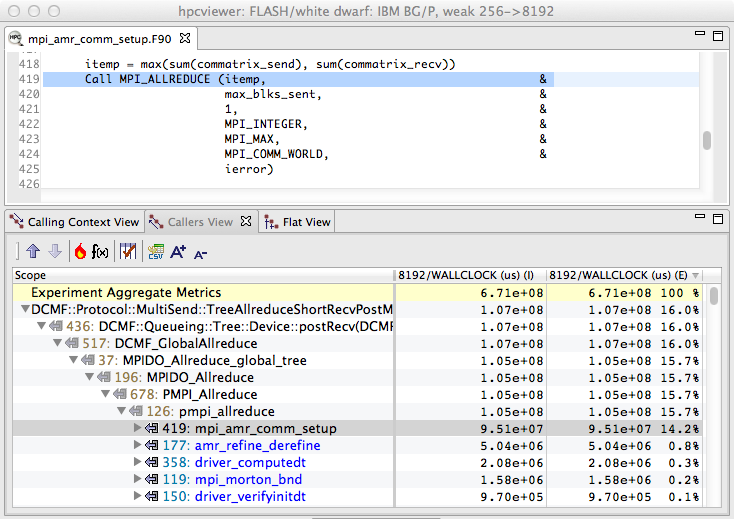
\includegraphics[width=.8\textwidth]{fig/hpctoolkit-code-centric}}
\caption{A code-centric view of an execution of the University of Chicago's FLASH code executing on 8192 cores of a Blue Gene/P. This bottom-up view shows that 16\% of the execution time was spent in IBM's DCMF messaging layer. By tracking these costs up the call chain, we can see that most of this time   was spent on behalf of calls to {\tt pmpi\_allreduce} on line 419 of {\tt amr\_comm\_setup}.}
\label{fig:code-centric}
\end{figure}

\begin{figure}[t]
\centering{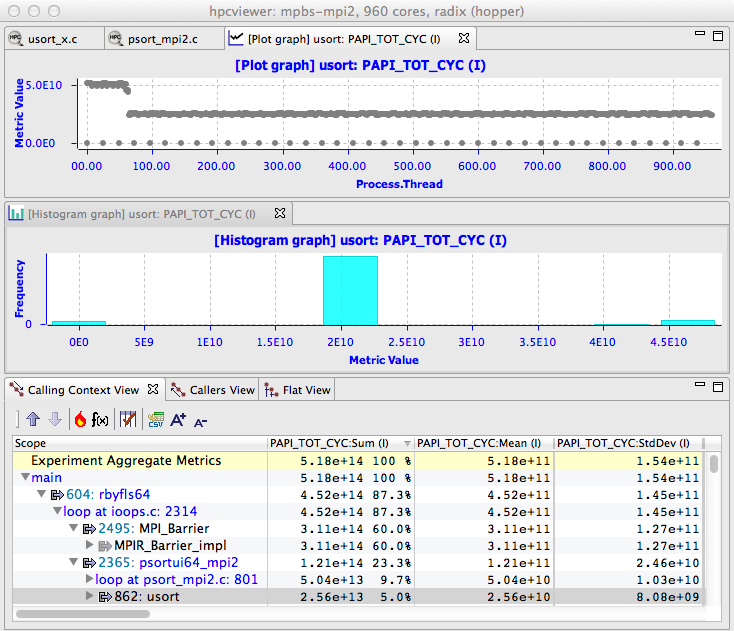
\includegraphics[width=.8\textwidth]{fig/hpctoolkit-thread-centric}}
\caption{A thread-centric view of the performance of a parallel radix sort application executing on 960 cores of a Cray XE6. The bottom pane shows a calling context for {\tt usort} in the execution. The top pane shows a graph of how much time each thread spent executing calls to {\tt usort} from the   highlighted context.  On a Cray XE6, there is one MPI helper thread for each compute node in the system; these helper threads spent no time executing {\tt usort}. The graph shows that some of the MPI ranks spent twice as much time in {\tt usort} as others. This happens because the radix sort divides up the work into 1024 buckets. In an execution on 960 cores,  896 cores work on one bucket and 64 cores work on two. The middle pane shows an alternate view of the thread-centric data as a histogram.}
\label{fig:thread-centric}
\end{figure}


\begin{figure}[t]
\centering{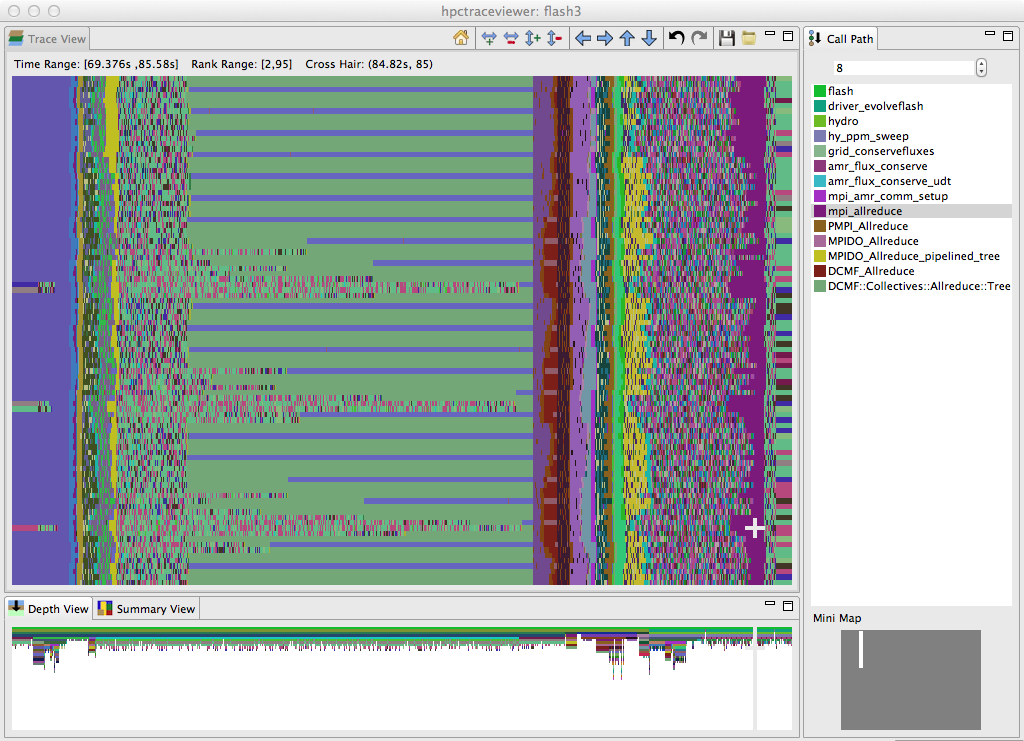
\includegraphics[width=.8\textwidth]{fig/hpctoolkit-time-centric}}
\caption{A time-centric view of  part of an execution of the University of Chicago's FLASH code  on 256 cores of a Blue Gene/P. The figure shows a detail from the end of the initialization phase and  part of the first iteration of the solve phase. The largest pane in the figure shows the activity of cores 2--95 in the execution during a time interval ranging from 69.376s--85.58s during the execution.  Time lines for threads are arranged from top to bottom and time flows from left to right. The color at any point in time for a thread indicates the procedure that the thread is executing at that time. The right pane shows the full call stack of thread 85 at 84.82s into the execution, corresponding to the selection shown by the white crosshair; the outermost procedure frame of the call stack is shown at the top of the pane and the innermost frame is shown at the bottom. This view highlights that even though FLASH is an SPMD program, the behavior of threads over time can be quite different. The purple region highlighted by the cursor, which represents a call by all processors to {\tt mpi\_allreduce}, shows that the time spent in this call varies across the processors. The variation in time spent waiting in {\tt mpi\_allreduce} is readily explained by an imbalance in the time processes spend a prior prolongation step, shown in yellow. Further left in the figure, one can see differences among ranks executing on different cores in each node as they await the  completion of an {\tt mpi\_allreduce}. A rank executing on one core of each node waits in {\tt DCMF\_Messager\_advance} (which appears as blue stripes) while ranks executing on other cores in each node wait in a helper function (shown in green). In this phase, ranks await the delayed arrival of a few of their peers who have extra work to do inside {\tt simulation\_initblock} before they call  {\tt mpi\_allreduce}. }
\label{fig:time-centric}
\end{figure}





By working at the machine-code level, \HPCToolkit{} accurately measures and attributes costs in executions of multilingual programs, even if they are linked with libraries available only in binary form.
\HPCToolkit{} supports performance analysis of fully optimized code -- the only form of a program worth measuring; it even measures and attributes performance metrics to shared libraries that are dynamically loaded at run time.
The low overhead of \HPCToolkit{}'s sampling-based measurement is particularly important for parallel programs because measurement overhead can distort program behavior.

\HPCToolkit{} is also especially good at pinpointing scaling losses in parallel codes, both within multicore nodes and across the nodes in a parallel system.
Using differential analysis of call path profiles collected on different numbers of threads or processes enables one to quantify scalability losses and pinpoint their causes to individual lines of code executed in particular calling contexts~\cite{Coarfa-MC:2007:ICS-scalability}.
We have used this technique to quantify scaling losses in leading science applications across thousands of processor cores on Cray and IBM Blue Gene systems, associate them with individual lines of source code in full calling context~\cite{Tallent-MC-etal:2009:SC-hpctoolkit-petascale,Tallent-MC-etal:2010:SC-hpctoolkit-load-imbalance}, and quantify scaling losses in science applications within compute nodes at the loop nest level due to competition for memory bandwidth in multicore processors~\cite{Tallent-etal:2008:SciDAC-hpctoolkit}.
We have also developed techniques for efficiently attributing the idleness in one thread to its cause in another thread~\cite{Tallent-MC:2009:PPoPP-hpctoolkit-work-stealing,Tallent-MC-Porterfield:2010:PPoPP-hpctoolkit-lock-contention}.

\HPCToolkit{} is deployed on many DOE supercomputers, including 
the Sierra supercomputer (IBM Power9 + NVIDIA V100 GPUs) at Lawrence Livermore National Laboratory,
Cray XC40 systems at Argonne's Leadership Computing Facility and the National Energy
Research Scientific Computing Center; the Summit supercomputer (IBM Power9 + NVIDIA V100 GPUs) at Oak Ridge Leadership Computing Facility, 
Blue Gene/Q systems at Argonne Leadership Computing Facility, 
as well as other clusters and supercomputers based on x86\_64, Power, and ARM processors. 

% ***************************************************************************
% ***************************************************************************

\chapter{\HPCToolkit{} Overview}


\begin{figure}[t]
\centering{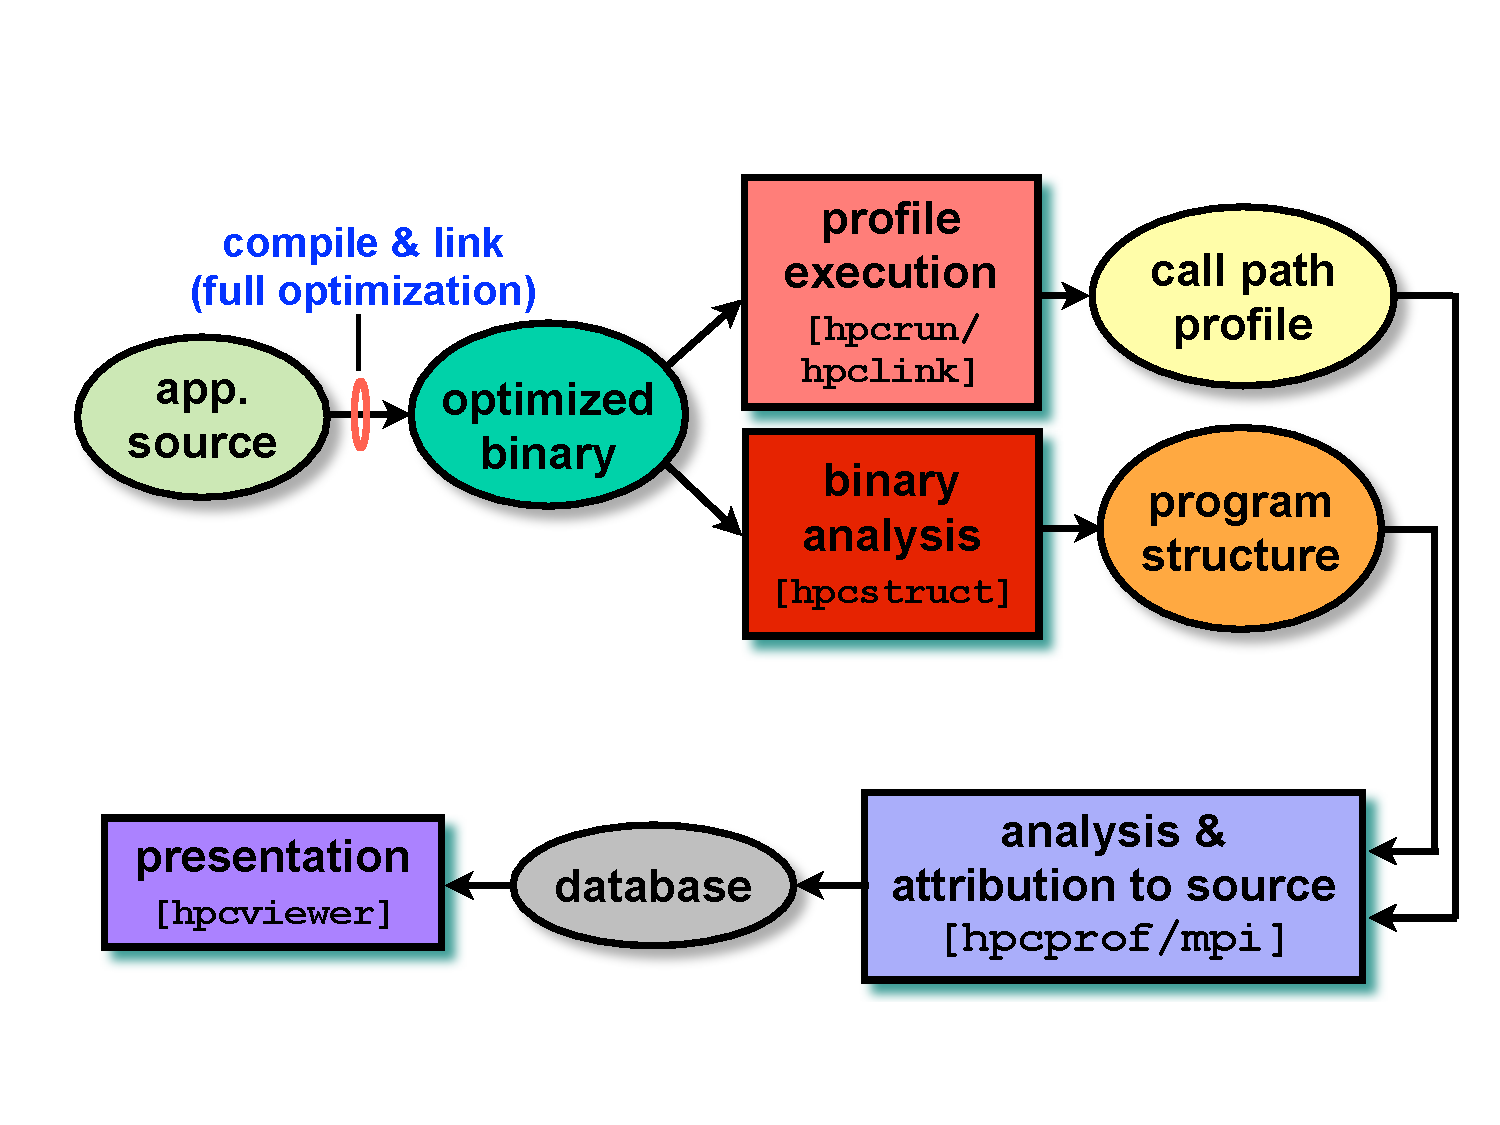
\includegraphics[width=.8\textwidth]{fig/hpctoolkit-workflow}}
\caption{Overview of \HPCToolkit{}'s tool work flow.}

\label{fig:hpctoolkit-overview:a}
\end{figure}

\HPCToolkit{}'s work flow is organized around four principal capabilities, as shown in Figure~\ref{fig:hpctoolkit-overview:a}:
\begin{enumerate}
  \item \emph{measurement} of context-sensitive performance metrics using call-stack unwinding 
while an application executes;
  \item \emph{binary analysis} to recover program structure from application binaries;
  \item \emph{attribution} of performance metrics by correlating dynamic performance metrics with static program structure; and
  \item \emph{presentation} of performance metrics and associated source code.
\end{enumerate}

To use \HPCToolkit{} to measure and analyze an application's performance, one first compiles and links the application for a production run, using \emph{full} optimization and including debugging symbols.%
\footnote{%
For the most detailed attribution of application performance data using \HPCToolkit{}, one should ensure that the compiler includes line map information in the object code it generates. While \HPCToolkit{} does not need this information to function, it can be helpful to users trying to interpret the results. Since compilers can usually provide line map information for fully optimized code, this requirement need not require a special build process. For instance, with the Intel compiler we recommend using \texttt{-g -debug inline\_debug\_info}.}
Second, one launches an application with \HPCToolkit{}'s measurement tool, \hpcrun{}, which uses statistical sampling to collect a performance profile.
Third, one invokes \hpcstruct{}, \HPCToolkit{}'s tool for analyzing an application binary to recover information about files, procedures, loops, and inlined code.
Fourth, one uses \hpcprof{} to combine information about an application's structure with dynamic performance measurements to produce a performance database.
Finally, one explores a performance database with \HPCToolkit{}'s \hpcviewer{} and/or \hpctraceviewer{} graphical presentation tools.

The rest of this chapter briefly discusses unique aspects of \HPCToolkit{}'s measurement, analysis and presentation capabilities.


\section{Asynchronous Sampling}

Without accurate measurement, performance analysis results may be of questionable value.
As a result, a principal focus of work on \HPCToolkit{} has been the design and implementation of techniques to provide accurate fine-grain measurements of production applications running at scale.
For tools to be useful on production applications on large-scale parallel systems, large measurement overhead is unacceptable.
For measurements to be accurate, performance tools must avoid introducing measurement error.
Both source-level and binary instrumentation can distort application performance through a variety of mechanisms~\cite{Mytkowicz:2009:PWD:2528521.1508275}. 
Frequent calls to small instrumented procedures can lead to considerable measurement overhead.
Furthermore, source-level instrumentation can distort application performance by interfering with inlining and template optimization. 
To avoid these effects, many instrumentation-based tools intentionally refrain from instrumenting certain procedures.
Ironically, the more this approach reduces overhead, the more it introduces \emph{blind spots}, \ie{}, intervals of unmonitored execution.
For example, a common selective instrumentation technique is to ignore small frequently executed procedures --- but these may be just the thread synchronization library routines that are critical.
Sometimes, a tool unintentionally introduces a blind spot.
A typical example is that source code instrumentation suffers from blind spots when source code is unavailable, a common condition for math and communication libraries.

To avoid these problems, \HPCToolkit{} eschews instrumentation and favors the use of \emph{asynchronous sampling} to measure and attribute performance metrics.
During a program execution, sample events are triggered by periodic interrupts induced by an interval timer or overflow of hardware performance counters.
One can sample metrics that reflect work (\eg{}, instructions, floating-point operations), consumption of resources (\eg{}, cycles, bandwidth consumed in the memory hierarhcy by data transfers in response to cache misses), or inefficiency (\eg{}, stall cycles).
For reasonable sampling frequencies, the overhead and distortion introduced by sampling-based measurement is typically much lower than that introduced by instrumentation~\cite{Froyd-MC-Fo:2005:ICS-csprof}.


\section{Call Path Profiling}

For all but the most trivially structured programs, it is important to associate the costs incurred by each procedure with the contexts in which the procedure is called.
Knowing the context in which each cost is incurred is essential for understanding why the code performs as it does.
This is particularly important for code based on application frameworks and libraries.
For instance, costs incurred for calls to communication primitives (\eg{}, \mytt{MPI_Wait}) or code that results from instantiating C++ templates for data structures can vary widely depending how they are used in a particular context.
Because there are often layered implementations within applications and libraries, it is insufficient either to insert instrumentation at any one level or to distinguish costs based only upon the immediate caller.
For this reason, \HPCToolkit{} uses call path profiling to attribute costs to the full calling contexts in which they are incurred.

\HPCToolkit{}'s \hpcrun{} call path profiler uses call stack unwinding to attribute execution costs of optimized executables to the full calling context in which they occur.
Unlike other tools, to support asynchronous call stack unwinding during execution of optimized code, \hpcrun{} uses on-line binary analysis to locate procedure bounds and compute an unwind recipe for each code range within each procedure~\cite{Tallent-MC-Fagan:2009:PLDI-hpctoolkit-binary-analysis}.
These analyses enable \hpcrun{} to unwind call stacks for optimized code with little or no information other than an application's machine code. 

\begin{comment}
To attribute performance back to source code, \HPCToolkit{} combines a call path profile with information gleaned through post-mortem analysis of an application's object code and its debugging sections.
This post-mortem analysis of an executable recovers its program structure and reconstructs a mapping from instructions back to source lines, loops, inlined functions, and procedures.
\HPCToolkit{}'s ability to attribute costs to dynamic call paths, including loops and inlined functions, for optimized code without a special-purpose compiler is unique.
\end{comment}


\section{Recovering Static Program Structure}

To enable effective analysis, call path profiles for executions of optimized programs must be correlated with important source code abstractions.
Since measurements refer only to instruction addresses within an executable, it is necessary to map measurements back to the program source.
To associate measurement data with the static structure of fully-optimized executables, we need a mapping between object code and its associated source code structure.%
\footnote{This object to source code mapping should be contrasted with the binary's line map, which (if present) is typically fundamentally line based.}
\HPCToolkit{} constructs this mapping using binary analysis; we call this process \emph{recovering program structure}~\cite{Tallent-MC-Fagan:2009:PLDI-hpctoolkit-binary-analysis}.

\HPCToolkit{} focuses its efforts on recovering procedures, inlined functions and templates, as well as  loop nests, the most important elements of source code structure.
To recover program structure, \HPCToolkit's \hpcstruct{} utility parses a load module's machine instructions, reconstructs a control flow graph, combines line map and DWARF information about inlining with interval analysis on the control flow graph in a way that enables it to relate machine code after optimization back to the original source~\cite{Tallent-MC-Fagan:2009:PLDI-hpctoolkit-binary-analysis}.
%\footnote{Without line map information, \hpcstruct{} can still identify procedures and loops, but is not able to account for inlining or loop transformations.}

Two important benefits naturally accrue from this approach.
First, \HPCToolkit{} can expose the structure of and assign metrics to what is actually executed, \emph{even if source code is unavailable}.
For example, \hpcstruct{}'s program structure naturally reveals transformations such as loop fusion and scalarization loops that arise from compilation of Fortran 90 array notation.
Similarly, it exposes calls to compiler support routines and wait loops in communication libraries of which one would otherwise be unaware.
%\hpcrun{}'s function discovery heuristics expose distinct logical procedures within stripped binaries.
Second, we combine (post-mortem) the recovered static program structure with dynamic call paths to expose inlined frames and loop nests.
This enables us to attribute the performance of samples in their full static and dynamic context and correlate it with source code.


\section{Presenting Performance Measurements}

To enable an analyst to rapidly pinpoint and quantify performance bottlenecks, tools must present the performance measurements in a way that engages the analyst, focuses attention on what is important, and automates common analysis subtasks to reduce the mental effort and frustration of sifting through a sea of measurement details.

To enable rapid analysis of an execution's performance bottlenecks, we have carefully designed the \hpcviewer{} - a code-centric presentation tool~\cite{Adhianto-MC-Ta:2010:PSTI-hpcviewer} and \hpctraceviewer{} - a time-centric presentation tool~\cite{Tallent-MC-etal:2011:ICS-hpctoolkit-scalable-tracing}. 

\hpcviewer{} combines a relatively small set of complementary presentation techniques that, taken together, rapidly focus an analyst's attention on performance bottlenecks rather than on unimportant information.
To facilitate the goal of rapidly focusing an analyst's attention on performance bottlenecks \hpcviewer{} extends several existing presentation techniques.
In particular, \hpcviewer{} (1) synthesizes and presents three complementary views of calling-context-sensitive metrics; (2) treats a procedure's static structure as first-class information with respect to both performance metrics and constructing views; (3) enables a large variety of user-defined metrics to describe performance inefficiency; and (4) automatically expands hot paths based on arbitrary performance metrics --- through calling contexts and static structure --- to rapidly highlight important performance data.

\hpctraceviewer{}  enables an application developer to visualize how a parallel execution unfolds over time. This view facilitates identification of important inefficiencies such as serialization and load imbalance, among others.



% ***************************************************************************
% ***************************************************************************

\chapter{Quick Start}
\label{chpt:quickstart}

This chapter provides a rapid overview of analyzing the performance of an application using \HPCToolkit{}.
It assumes an operational installation of \HPCToolkit{}.


% ===========================================================================
% ===========================================================================

\section{Guided Tour}
\label{chpt:quickstart:tour}

\begin{figure}[t]
\centering{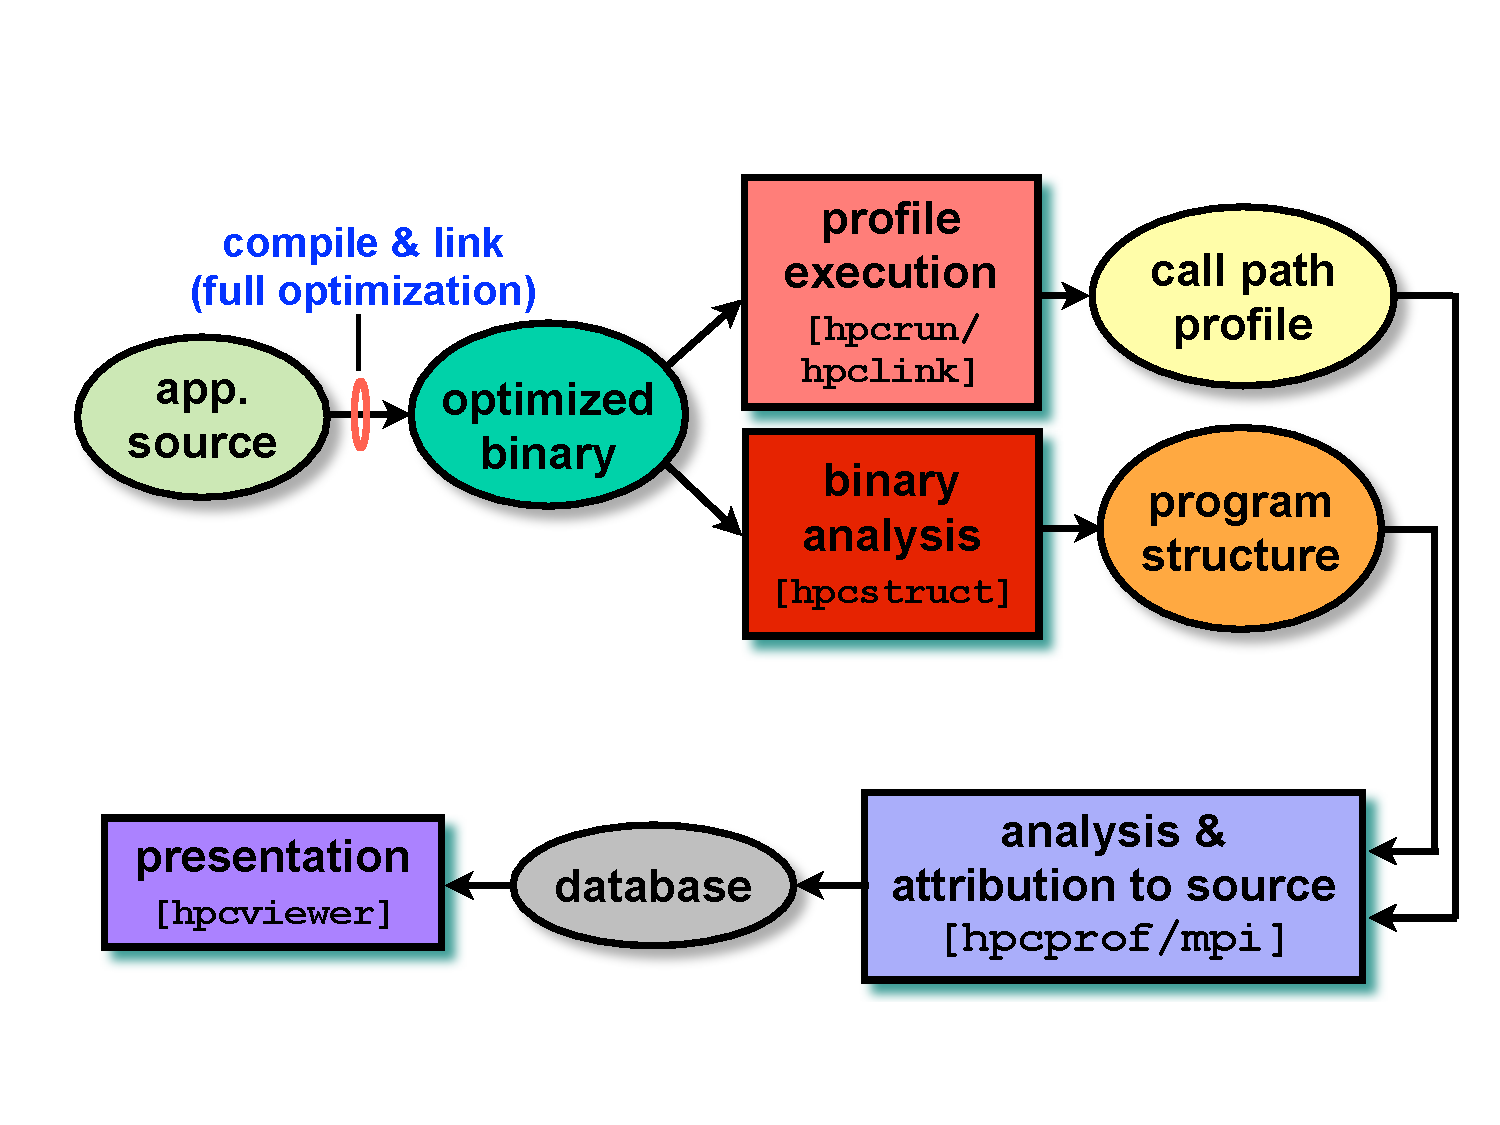
\includegraphics[width=.8\textwidth]{fig/hpctoolkit-workflow}}
\caption{Overview of \HPCToolkit{} tool's work flow.}
\label{fig:hpctoolkit-overview:b}
\end{figure}

\HPCToolkit{}'s work flow is summarized in Figure~\ref{fig:hpctoolkit-overview:b} (on page~\pageref{fig:hpctoolkit-overview:b}) and is organized around four principal capabilities:
\begin{enumerate}
  \item \emph{measurement} of context-sensitive performance metrics while an application executes;
  \item \emph{binary analysis} to recover program structure from application binaries;
  \item \emph{attribution} of performance metrics by correlating dynamic performance metrics with static program structure; and
  \item \emph{presentation} of performance metrics and associated source code.
\end{enumerate}

To use \HPCToolkit{} to measure and analyze an application's performance, one first compiles and links the application for a production run, using \emph{full} optimization.
Second, one launches an application with \HPCToolkit{}'s measurement tool, \hpcrun{}, which uses statistical sampling to collect a performance profile.
Third, one invokes \hpcstruct{}, \HPCToolkit{}'s tool for analyzing an application binary to recover information about files, procedures, loops, and inlined code.
Fourth, one uses \hpcprof{} to combine information about an application's structure with dynamic performance measurements to produce a performance database.
For large executions where analyzing performance measurements serially would be imprudent, \HPCToolkit{}  provides \hpcprofmpi{} - an MPI program that can be launched to analyze  performance data from many MPI ranks and threads in parallel.
Finally, one explores a performance database with one of \HPCToolkit{}'s graphical user interfaces: \hpcviewer{} for code-centric analysis of performance metrics or  \hpctraceviewer{} for time-centric analysis of an execution. 

The following subsections explain \HPCToolkit{}'s work flow in more detail.


% ==========================================================
% ==========================================================

\subsection{Compiling an Application}

For the most detailed attribution of application performance data using \HPCToolkit{}, one should compile so as to include with line map information in the generated object code.
This usually means compiling with options similar to `\texttt{-g -O3}'. Check your compiler's documentation for information about the right set of options to have the compiler record information about inlining and the mapping of machine instructions to source lines. We advise picking  options that indicate they will record information that relates machine instructions to source code without compromising optimization. For instance, the Portland Group (PGI) compilers, use \texttt{-gopt} in place of \texttt{-g} to collect information without interfering with optimization.

While \HPCToolkit{} does not need information about the mapping between machine instructions and source code to function, having such information included in the binary code by the compiler can be helpful to users trying to interpret performance measurements.
Since compilers can usually provide information about line mappings and inlining for fully-optimized code, this requirement usually involves a one-time trivial adjustment to the an application's build scripts to provide a better experience with tools. Such mapping information enables tools such as \HPCToolkit{}, race detectors, and memory analysis tools to attribute information more precisely.


% ==========================================================
% ==========================================================

\subsection{Measuring Application Performance}
\label{chpt:quickstart:tour:measurement}

Measurement of application performance takes two different forms depending on whether your application is dynamically or statically linked.
To monitor a dynamically linked application, simply use \hpcrun{} to launch the application.
To monitor a statically linked application, such as those typically used on Blue Gene and Cray supercomputers, link your application using \hpclink{}.
In either case, the application may be sequential, multithreaded or based on MPI.
The commands below give examples for an application named \texttt{app}.
%
\begin{itemize}

\item Dynamically linked applications:\hfill

Simply launch your application with \hpcrun{}:
\begin{quote}
  \verb|[<mpi-launcher>] hpcrun [hpcrun-options] app [app-arguments]|
\end{quote}
Of course, \texttt{<mpi-launcher>} is only needed for MPI programs and is sometimes a program like \texttt{mpiexec} or \texttt{mpirun}, or a workload manager's utilities such as Slurm's {\tt srun} or IBM's Job Step Manager utility {\tt jsrun}.

\item Statically linked applications:\hfill

First, link \hpcrun{}'s monitoring code into \texttt{app}, using \hpclink{}:
\begin{quote}
  \verb|hpclink <linker> -o app <linker-arguments>|
\end{quote}

Then monitor \texttt{app} by passing \hpcrun{} options through environment variables.
For instance:
\begin{quote}
\begin{verbatim}
export HPCRUN_EVENT_LIST="CYCLES"
[<mpi-launcher>] app [app-arguments]
\end{verbatim}
\end{quote}
\hpclink{}'s \mytt{--help} option gives a list of environment variables that affect monitoring.
See Chapter~\ref{chpt:statically-linked-apps} for more information.

\end{itemize}
%
Any of these commands will produce a measurements database that contains separate measurement information for each MPI rank and thread in the application.
The database is named according the form:
\begin{quote}
  \verb|hpctoolkit-app-measurements[-<jobid>]|
\end{quote}
If the application \texttt{app} is run under control of a recognized batch job scheduler (such as Slurm, Cobalt, or IBM's Job Manager), the name of the measurements directory will contain the corresponding job identifier \texttt{<jobid>}.
Currently, the database contains measurements files for each thread that are named using the following templates:
\begin{quote}
  \verb|app-<mpi-rank>-<thread-id>-<host-id>-<process-id>.<generation-id>.hpcrun|
    \verb|app-<mpi-rank>-<thread-id>-<host-id>-<process-id>.<generation-id>.hpctrace|
\end{quote}

\subsubsection{Specifying Sample Sources}

\HPCToolkit{} primarily monitors an application using asynchronous sampling.
Consequently, the most common option to \hpcrun{} is a list of sample sources that define how samples are generated.
A sample source takes the form of an event name $e$ and \texttt{howoften}, specified as \texttt{$e$@howoften}. The specifier \texttt{howoften} may 
be a number, indicating a period, \eg{} \mytt{CYCLES@4000001} or it may be \texttt{f} followed by a number, \mytt{CYCLES@f200} indicating a frequency in samples/second.
For a sample source with event $e$ and period $p$, after every \emph{p} instances of \emph{e}, a sample is generated that causes \hpcrun{} to inspect the and record information about the monitored application.

To configure \hpcrun{} with two samples sources, \texttt{$e_1$@howoften$_1$} and \texttt{$e_2$@howoften$_2$}, use the following options:
\begin{quote}
  \texttt{--event $e_1$@howoften$_1$ --event $e_2$@howoften$_2$}
\end{quote}
To use the same sample sources with an \hpclink{}-ed application, use a command similar to:
\begin{quote}
  \texttt{export HPCRUN\_EVENT\_LIST="$e_1$@howoften$_1$ $e_2$@howoften$_2$"}
\end{quote}


% ==========================================================
% ==========================================================

\subsection{Recovering Program Structure}

To recover static program structure for the application \texttt{app}, use the command:
\begin{quote}
  \verb|hpcstruct app|
\end{quote}
This command analyzes \texttt{app}'s binary and computes a representation of its static source code structure, including its loop nesting structure.
The command saves this information in a file named \texttt{app.hpcstruct} that should be passed to \hpcprof{} with the \texttt{-S/--structure} argument.

Typically, \hpcstruct{} is launched without any options.
% When using an IBM XL compiler, it is usually best to pass the option \texttt{--loop-fwd-subst=no} to \hpcstruct{}.


% ==========================================================
% ==========================================================

\subsection{Analyzing Measurements \& Attributing Them to Source Code}

To analyze \HPCToolkit{}'s measurements and attribute them to the application's source code, use either \hpcprof{} or \hpcprofmpi{}.
In most respects, \hpcprof{} and \hpcprofmpi{} are semantically idential. For convenience, we use the notation \hpcprofAll{} to refer to both of these tools.
Both generate the same set of summary metrics over all threads and processes in an execution.
The difference between the two is that the latter is designed to process (in parallel) measurements from large-scale executions.
Consequently, while the former can optionally generate separate metrics for each thread (see the \mytt{--metric/-M} option), the latter only generates summary metrics.
However, the latter can also generate additional information for plotting thread-level metric values (see Section~\ref{sec:hpcviewer:plots}%
%s~\ref{sec:effective-performance-analysis:load-imbalance} and
).

\hpcprof{} is typically used as follows:
\begin{quote}
\begin{verbatim}
hpcprof -S app.hpcstruct -I <app-src>/+ \
  hpctoolkit-app-measurements1 [hpctoolkit-app-measurements2 ...]
\end{verbatim}
\end{quote}
and \hpcprofmpi{} is analogous:
\begin{quote}
\begin{verbatim}
<mpi-launcher> hpcprof-mpi \
  -S app.hpcstruct -I <app-src>/+ \
  hpctoolkit-app-measurements1 [hpctoolkit-app-measurements2 ...]
\end{verbatim}
\end{quote}
Either command will produce an \HPCToolkit{} performance database with the name \texttt{hpctoolkit-app-database}.
If this database directory already exists, \hpcprofAll{} will form a unique name using a numerical qualifier.

Both \hpcprofAll{} can collate multiple measurement databases, as long as they are gathered against the same binary.
This capability is useful for (a) combining event sets gathered over multiple executions and (b) performing scalability studies (see Section~\ref{sec:effective-performance-analysis:scalability}).

The above commands use two important options.
The \texttt{-S/--structure} option takes a program structure file.
The \texttt{-I/--include} option takes a directory \texttt{<app-src>} to application source code; the optional `\texttt{+}' suffix requests that the directory be searched recursively for source code.
Either option can be passed multiple times to specify multiple structure files (e.g., for the application and each of the key libraries it uses) or multiple include paths that indicate  roots of source trees for the application and/or of its libraries. 

Another potentially important option, especially for machines that require executing from special file systems, is the \texttt{-R/--replace-path} option for substituting instances of \emph{old-path} with \emph{new-path}: \texttt{-R 'old-path=new-path'}.

A possibly important detail about the above command is that source code should be considered an \hpcprofAll{} input.
This is critical when using a machine that restricts executions to a scratch parallel file system.
In such cases, not only must you copy \hpcprofmpi{} into the scratch file system, but also all source code that you want \hpcprofmpi{} to find and copy into the resulting Experiment database.


% ==========================================================
% ==========================================================

\subsection{Presenting Performance Measurements for Interactive Analysis}

To interactively view and analyze an \HPCToolkit{} performance database, use \hpcviewer{}.
\hpcviewer{} may be launched from the command line or by double-clicking on its icon on MacOS or Windows.
The following is an example of launching from a command line:
\begin{quote}
  \verb|hpcviewer hpctoolkit-app-database|
\end{quote}
Additional help for \hpcviewer{} can be found in a help pane available from \hpcviewer{}'s \emph{Help} menu.

% ==========================================================
% ==========================================================

\subsection{Effective Performance Analysis Techniques}

To effectively analyze application performance, consider using one of the following strategies, which are described in more detail in Chapter~\ref{chpt:effective-performance-analysis}.
\begin{itemize}
\item
A waste metric, which represents the difference between achieved performance and potential peak performance is a good way of understanding the potential for tuning the node performance of codes (Section~\ref{sec:effective-performance-analysis:inefficiencies}).
\hpcviewer{} supports synthesis of derived metrics to aid analysis.
Derived metrics are specified within \hpcviewer{} using spreadsheet-like formula.
See the \hpcviewer{} help pane for details about how to specify derived metrics.

\item
Scalability bottlenecks in parallel codes can be pinpointed by differential analysis of two profiles with different degrees of parallelism (Section~\ref{sec:effective-performance-analysis:scalability}).

The following sketches the mechanics of performing a simple scalability study between executions $x$ and $y$ of an application \texttt{app}:
\begin{quote}
  \verb|hpcrun [options-x] app [app-arguments-x]| \hfill (execution $x$) \\
  \verb|hpcrun [options-y] app [app-arguments-y]| \hfill (execution $y$) \\
  \verb|hpcstruct app| \\
  \verb|hpcprof/mpi -S ... -I ... measurements-x measurements-y| \\
  \verb|hpcviewer hpctoolkit-database| \hfill (compute a scaling-loss metric)
\end{quote}

\end{itemize}


% ===========================================================================
% ===========================================================================

\section{Additional Guidance}

For additional information, consult the rest of this manual and other documentation:
First, we summarize the available documentation and command-line help:

\begin{description}

\item[Command-line help.]\hfill

Each of \HPCToolkit{}'s command-line tools can generate a help message summarizing the tool's usage, arguments and options.
To generate this help message, invoke the tool with \mytt{-h} or \mytt{--help}.

\item[Man pages.]\hfill

Man pages are available either via the Internet (\url{http://hpctoolkit.org/documentation.html}) or from a local \HPCToolkit{} installation (\mytt{<hpctoolkit-installation>/share/man}).

\item[Manuals.]\hfill

Manuals are available either via the Internet (\url{http://hpctoolkit.org/documentation.html}) or from a local \HPCToolkit{} installation (\mytt{<hpctoolkit-installation>/share/doc/hpctoolkit/documentation.html}).

\item[Articles and Papers.]\hfill

There are a number of articles and papers that describe various aspects of \HPCToolkit{}'s measurement, analysis, attribution and presentation technology.
They can be found at \url{http://hpctoolkit.org/publications.html}.

\end{description}


% ***************************************************************************
% ***************************************************************************

\chapter{Effective Strategies for Analyzing Program Performance}
\label{chpt:effective-performance-analysis}

This chapter describes some proven strategies for using performance measurements to identify performance bottlenecks in both serial and parallel codes.


% ===========================================================================
% ===========================================================================

\section{Monitoring High-Latency Penalty Events}
\label{sec:effective-performance-analysis:penalty-events}

A very simple and often effective methodology is to profile with respect to cycles and high-latency penalty events.
If \HPCToolkit{} attributes a large number of penalty events with a particular source-code statement, there is an extremely high likelihood of significant exposed stalling.
This is true even though (1) modern out-of-order processors can overlap the stall latency of one instruction with nearby independent instructions and (2) some penalty events ``over count''.%
\footnote{For example, performance monitoring units often categorize a prefetch as a cache miss.}
If a source-code statement incurs a large number of penalty events and it also consumes a non-trivial amount of cycles, then this region of code is an opportunity for optimization.
Examples of good penalty events are last-level cache misses and TLB misses.


% ===========================================================================
% ===========================================================================

\section{Computing Derived Metrics}
\label{sec:effective-performance-analysis:derived-metrics}

Modern computer systems provide access to a rich set of hardware performance counters that can directly measure various aspects of a program's performance.
Counters in the processor core and memory hierarchy enable one to collect measures of work (\eg, operations performed), resource consumption (\eg, cycles), and inefficiency (\eg, stall cycles).
One can also measure time using system timers.

Values of individual metrics are of limited use by themselves.
For instance, knowing the count of cache misses for a loop or routine is of little value by itself; only when combined with other information such as the number of instructions executed or the total number of cache accesses does the data become informative.
While a developer might not mind using mental arithmetic to evaluate the relationship between a pair of metrics for a particular program scope (\eg, a loop or a procedure), doing this for many program scopes is exhausting.
To address this problem, \hpcviewer{} supports calculation of derived metrics.
\hpcviewer{} provides an interface that enables a user to specify spreadsheet-like formula that can be used to calculate a derived metric for every program scope. 

% For instance, if one wants to compute the cache miss rate in a scope, one could divide the total number of cache misses in a scope by the sum of counts of loads and stores in the scope. On the other hand, if one wanted to compute the fraction of a program's cache misses that occurred in a particular scope, one could divide the number of misses in the scope by the total number of misses in the program.

\begin{figure}[t]
\center{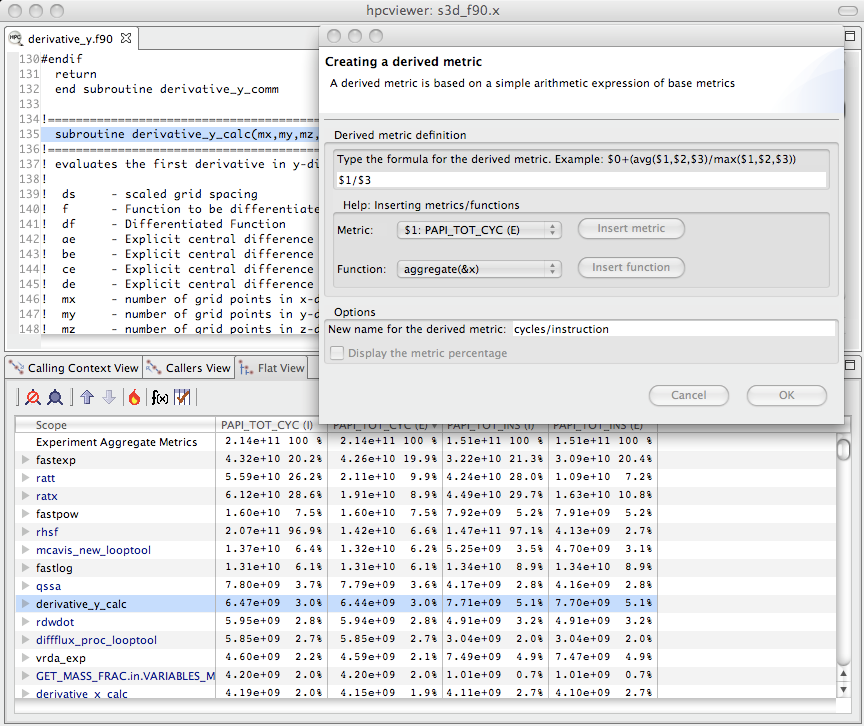
\includegraphics[width=1.0\textwidth]{fig/cycles-per-inst.png}}
%Two possible representations for the call path fragment $\ldots s_1 \rightarrow s_2 \ldots$, where $s_1$ and $s_2$ are call sites and where $s_1$ represents a call from $p$ to $q$ and $s_2$ a call from $q'$ to $r$.
\caption{Computing a derived metric (cycles per instruction) in \hpcviewer{}.}
\label{fig:cycles-per-inst}
\end{figure}

Figure~\ref{fig:cycles-per-inst} shows how to use \hpcviewer{} to compute a \emph{cycles}/\emph{instruction} derived metric from measured metrics \mytt{PAPI_TOT_CYC} and \mytt{PAPI_TOT_INS}; these metrics correspond to {\em cycles} and {\em total instructions executed} measured with the PAPI hardware counter interface.
To compute a derived metric, one first depresses the button marked $f(x)$ above the metric pane; that will cause the pane for computing a derived metric to appear.
Next, one types in the formula for the metric of interest.
When specifying a formula, existing columns of metric data are referred to using a positional name \$$n$ to refer to the $n^{th}$ column, where the first column is written as \$0.
The metric pane shows the formula $\$1/\$3$.
Here, \$1 refers to the column of data representing the exclusive value for \mytt{PAPI_TOT_CYC} and \$3 refers to the column of data representing the exclusive value for \mytt{PAPI_TOT_INS}.%
\footnote{An {\em exclusive} metric for a scope refers to the quantity of the metric measured for that scope alone; an \emph{inclusive} metric for a scope represents the value measured for that scope as well as costs incurred by any functions it calls. In \hpcviewer{}, inclusive metric columns are marked with ``(I)'' and exclusive metric columns are marked with ``(E).''}
Positional names for metrics you use in your formula can be determined using the \emph{Metric} pull-down menu in the pane.
If you select your metric of choice using the pull-down, you can insert its positional name into the formula using the {\em insert metric} button, or you can simply type the positional name directly into the formula.

\begin{figure}[t]
\center{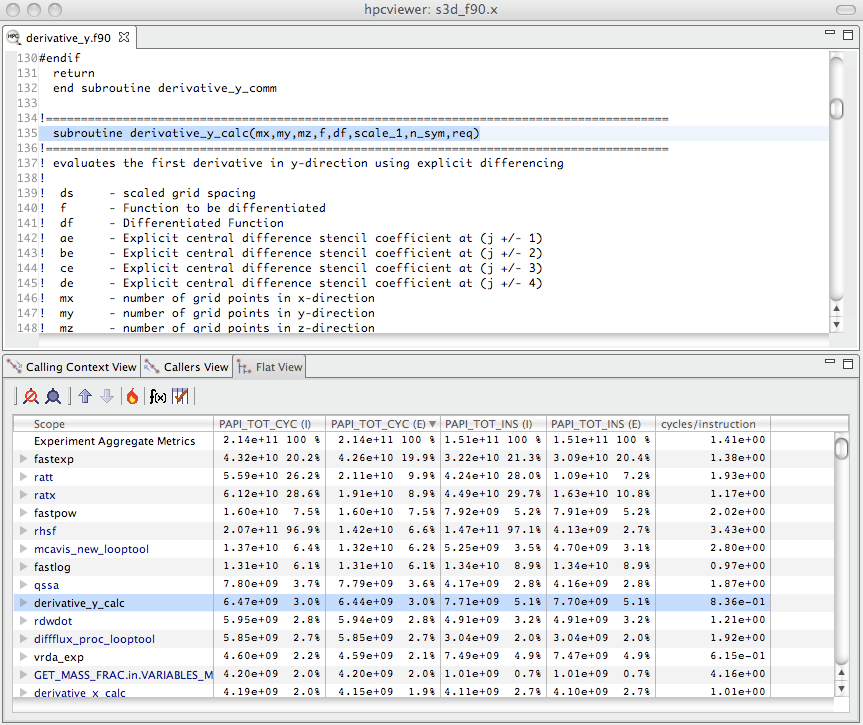
\includegraphics[width=1.0\textwidth]{fig/cycles-per-inst-2}}
%Two possible representations for the call path fragment $\ldots s_1 \rightarrow s_2 \ldots$, where $s_1$ and $s_2$ are call sites and where $s_1$ represents a call from $p$ to $q$ and $s_2$ a call from $q'$ to $r$.
\caption{Displaying the new {\em cycles/ instruction} derived metric in \hpcviewer{}.}
\label{fig:cycles-per-inst-2}
\end{figure}

At the bottom of the derived metric pane, one can specify a name for the new metric.
One also has the option to indicate that the derived metric column should report for each scope what percent of the total its quantity represents; for a metric that is a ratio, computing a percent of the total is not meaningful, so we leave the box unchecked.
After clicking the OK button, the derived metric pane will disappear and the new metric will appear as the rightmost column in the metric pane.
If the metric pane is already filled with other columns of metric, you may need to scroll right in the pane to see the new metric.
Alternatively, you can use the metric check-box pane (selected by depressing the button to the right of $f(x)$ above the metric pane) to hide some of the existing metrics so that there will be enough room on the screen to display the new metric.
Figure~\ref{fig:cycles-per-inst-2} shows the resulting \hpcviewer{} display after clicking OK to add the derived metric.

The following sections describe several types of derived metrics that are of particular use to gain insight into performance bottlenecks and opportunities for tuning.

% ===========================================================================
% ===========================================================================

\section{Pinpointing and Quantifying Inefficiencies}
\label{sec:effective-performance-analysis:inefficiencies}

While knowing where a program spends most of its time or executes most of its floating point operations may be interesting, such information may not suffice to identify the biggest targets of opportunity for improving program performance.
For program tuning, it is less important to know how much resources (\eg, time, instructions) were consumed in each program context than knowing where resources were consumed {\em inefficiently}.

To identify performance problems, it might initially seem appealing to compute ratios to see how many events per cycle occur in each program context.
For instance, one might compute ratios such as FLOPs/cycle, instructions/cycle, or cache miss ratios.
However, using such ratios as a sorting key to identify inefficient program contexts can misdirect a user's attention.
There may be program contexts (\eg, loops) in which computation is terribly inefficient (\eg, with low operation counts per cycle); however, some or all of the least efficient contexts may not account for a significant amount of execution time.
Just because a loop is inefficient doesn't mean that it is important for tuning. 

The best opportunities for tuning are where the aggregate performance losses are greatest.
For instance, consider a program with two loops.
The first loop might account for 90\% of the execution time and run at 50\% of peak performance.
The second loop might account for 10\% of the execution time, but only achieve 12\% of peak performance.
In this case, the total performance loss in the first loop accounts for 50\% of the first loop's execution time, which corresponds to 45\% of the total program execution time.
The 88\% performance loss in the second loop would account for only 8.8\% of the program's execution time.
In this case, tuning the first loop has a greater potential for improving the program performance even though the second loop is less efficient.

A good way to focus on inefficiency directly is with a derived {\em waste} metric.
Fortunately, it is easy to compute such useful metrics.
However, there is no one {\em right} measure of waste for all codes.
Depending upon what one expects as the rate-limiting resource (\eg, floating-point computation, memory bandwidth, etc.), one can define an appropriate waste metric (\eg, FLOP opportunities missed, bandwidth not consumed) and sort by that.


\begin{figure}[t]
\center{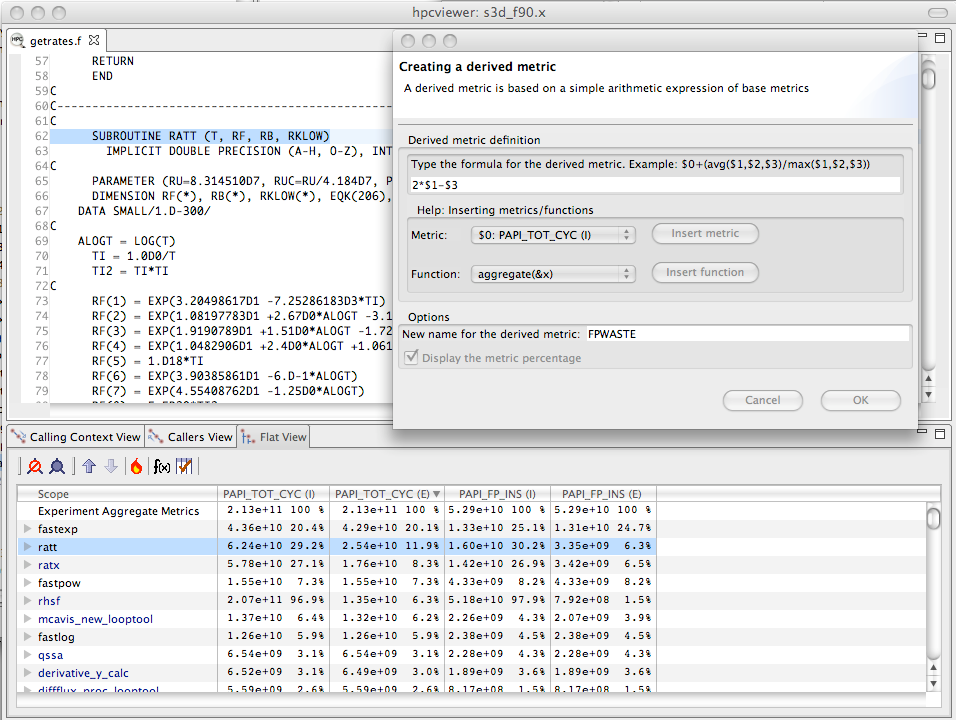
\includegraphics[width=1.0\textwidth]{fig/fpwaste.png}}
%Two possible representations for the call path fragment $\ldots s_1 \rightarrow s_2 \ldots$, where $s_1$ and $s_2$ are call sites and where $s_1$ represents a call from $p$ to $q$ and $s_2$ a call from $q'$ to $r$.
\caption{Computing a floating point waste metric in \hpcviewer{}.}
\label{fig:fpwaste}
\end{figure}

For instance, in a floating-point intensive code, one might consider keeping the floating point pipeline full as a metric of success.
One can directly quantify and pinpoint losses from failing to keep the floating point pipeline full {\em regardless of why this occurs}.
One can pinpoint and quantify losses of this nature by computing a {\em floating-point waste} metric that is calculated as the difference between the potential number of calculations that could have been performed if the computation was running at its peak rate minus the actual number that were performed.
To compute the number of calculations that could have been completed in each scope, multiply the total number of cycles spent in the scope by the peak rate of operations per cycle.
Using \hpcviewer{}, one can specify a formula to compute such a derived metric and it will compute the value of the derived metric for every scope.
Figure~\ref{fig:fpwaste} shows the specification of this floating-point waste metric for a code.\footnote{Many recent processors have trouble accurately counting floating-point operations accurately, which is unfortunate. If your processor can't accurately count floating-point operations, a floating-point waste metric will be less useful.}

Sorting by a waste metric will rank order scopes to show the scopes with the greatest waste.
Such scopes correspond directly to those that contain the greatest opportunities for improving overall program performance.
A waste metric will typically highlight loops where
\begin{itemize}
\item a lot of time is spent computing efficiently, but the aggregate inefficiencies accumulate,
\item less time is spent computing, but the computation is rather inefficient, and
\item scopes such as copy loops that contain no computation at all, which represent a complete waste according to a metric such as floating point waste.
\end{itemize}

\begin{figure}[t]
\center{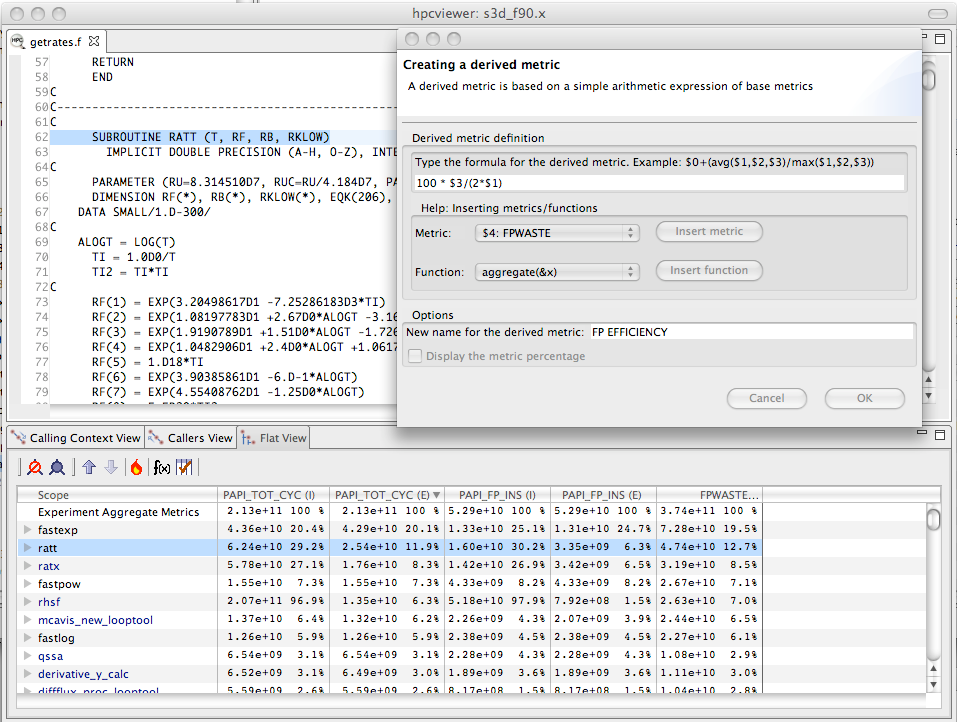
\includegraphics[width=1.0\textwidth]{fig/fp-efficiency.png}}
%Two possible representations for the call path fragment $\ldots s_1 \rightarrow s_2 \ldots$, where $s_1$ and $s_2$ are call sites and where $s_1$ represents a call from $p$ to $q$ and $s_2$ a call from $q'$ to $r$.
\caption{Computing floating point efficiency in percent using \hpcviewer{}.}
\label{fig:fpefficiency}
\end{figure}

Beyond identifying and quantifying opportunities for tuning with a waste metric, one can compute a companion derived metric {\em relative efficiency} metric to help understand how easy it might be to improve performance.
A scope running at very high efficiency will typically be much harder to tune than running at low efficiency.
For our floating-point waste metric, we one can compute the floating point efficiency metric by dividing measured FLOPs by potential peak FLOPs and multiplying the quantity by 100.
Figure~\ref{fig:fpefficiency} shows the specification of this floating-point efficiency metric for a code.

\begin{figure}[t]
\center{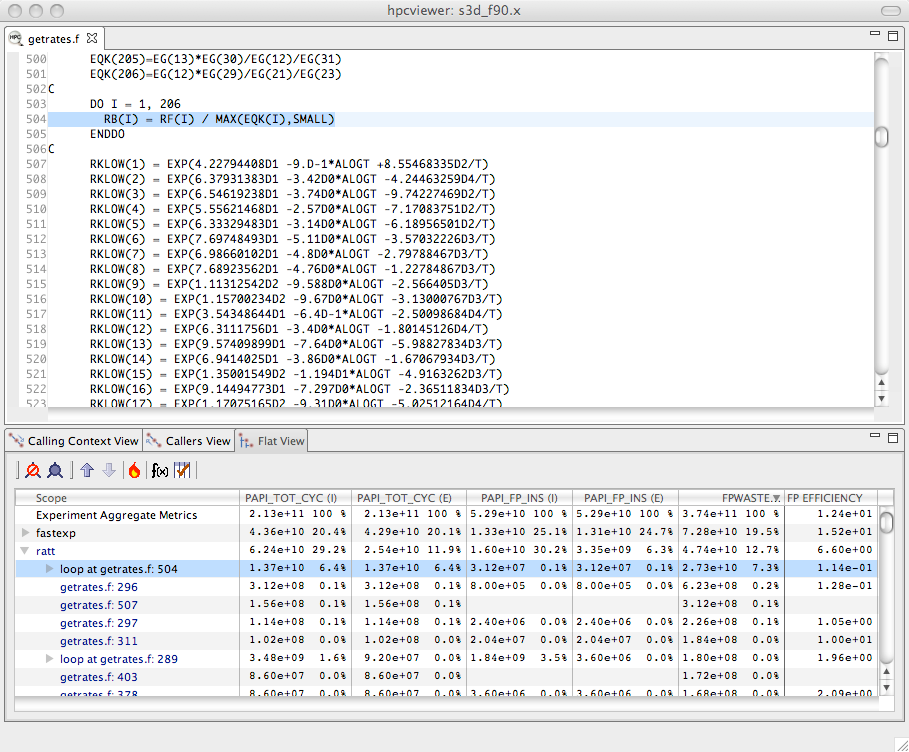
\includegraphics[width=1.0\textwidth]{fig/fp-efficiency-loop.png}}
%Two possible representations for the call path fragment $\ldots s_1 \rightarrow s_2 \ldots$, where $s_1$ and $s_2$ are call sites and where $s_1$ represents a call from $p$ to $q$ and $s_2$ a call from $q'$ to $r$.
\caption{Using floating point waste and the percent of floating point efficiency to evaluate opportunities for optimization.}
\label{fig:fpefficiency-loop}
\end{figure}

Scopes that rank high according to a waste metric and low according to a companion relative efficiency metric often make the best targets for optimization.
Figure~\ref{fig:fpefficiency-loop} shows the specification of this floating-point efficiency metric for a code.
Figure~\ref{fig:fpefficiency-loop} shows an \hpcviewer{} display that shows the top two routines that collectively account for 32.2\% of the floating point waste in a reactive turbulent combustion code.
The second routine (\mytt{ratt}) is expanded to show the loops and statements within.
While the overall floating point efficiency for \mytt{ratt} is at 6.6\% of peak (shown in scientific notation in the \hpcviewer{} display), the most costly loop in \mytt{ratt} that accounts for 7.3\% of the floating point waste is executing at only 0.114\% efficiency.
 Identifying such sources of inefficiency is the first step towards improving performance via tuning.


% ===========================================================================
% ===========================================================================

\section{Pinpointing and Quantifying Scalability Bottlenecks}
\label{sec:effective-performance-analysis:scalability}

On large-scale parallel systems, identifying impediments to scalability is of paramount importance.
On today's systems fashioned out of multicore processors, two kinds of scalability are of particular interest: 
\begin{itemize}
\item scaling within nodes, and
\item scaling across the entire system. 
\end{itemize}
\HPCToolkit{} can be used to readily pinpoint both kinds of bottlenecks.
Using call path profiles collected by \hpcrun{}, it is possible to quantify and pinpoint scalability bottlenecks of any kind, {\em regardless of cause}.

To pinpoint scalability bottlenecks in parallel programs, we use {\em differential profiling} --- mathematically combining corresponding buckets of two or more execution profiles.
Differential profiling was first described by McKenney~\cite{McKenney:1999:differential}; he used differential profiling to compare two {\em flat} execution profiles.
Differencing of flat profiles is useful for identifying what parts of a program incur different costs in two executions.
Building upon McKenney's idea of differential profiling, we compare call path profiles of parallel executions at different scales to pinpoint scalability bottlenecks.
Differential analysis of call path profiles pinpoints not only differences between two executions (in this case scalability losses), but the contexts in which those differences occur.
Associating changes in cost with full calling contexts is particularly important for pinpointing context-dependent behavior.
Context-dependent behavior is common in parallel programs.
For instance, in message passing programs, the time spent by a call to \mytt{MPI_Wait} depends upon the context in which it is called.
Similarly, how the performance of a communication event scales as the number of processors in a parallel execution increases depends upon a variety of factors such as whether the size of the data transferred increases and whether the communication is collective or not.


% ==========================================================
% ==========================================================

\subsection{Scalability Analysis Using Expectations}

Application developers have expectations about how the performance of their code should scale as the number of processors in a parallel execution increases.
Namely,
\begin{itemize}
\item when different numbers of
processors are used to solve the same problem (strong scaling), one
expects an execution's speedup to increase linearly with the number of processors employed;
\item when
different numbers of processors are used but the amount of computation
per processor is held constant (weak scaling), one expects the execution
time on a different number of processors to be the same.
\end{itemize}

In both of these situations, a code developer can express their expectations for how performance will scale as a formula that can be used to predict execution performance on a different number of processors.
One's expectations about how overall application performance should scale can be applied to each context in a program
to pinpoint and quantify deviations from expected scaling.
Specifically, one can scale and difference the performance of an application on different numbers of processors to pinpoint contexts that are not scaling ideally.

To pinpoint and quantify scalability bottlenecks in a parallel application, we first use \hpcrun{} to a collect call path profile for an application on two different numbers of processors.
Let $E_p$ be an execution on $p$ processors and $E_q$ be an execution on $q$ processors.
Without loss of generality, assume that $q > p$.

In our analysis, we consider both {\it inclusive} and {\it exclusive} costs for CCT nodes.
The inclusive cost at $n$ represents the sum of all costs attributed to $n$ and any of its descendants in the CCT, and is denoted by $I(n)$.
The exclusive cost at $n$ represents the sum of all costs attributed strictly to $n$, and we denote it by $E(n)$.
If $n$ is an interior node in a CCT, it represents an invocation of a procedure.
If $n$ is a leaf in a CCT, it represents a statement inside some procedure. For leaves, their inclusive and exclusive costs are equal.

It is useful to perform scalability analysis for both inclusive and exclusive costs; if the loss of scalability attributed to the inclusive costs of a function invocation is roughly equal to the loss of scalability due to its exclusive costs, then we know that the computation in that function invocation does not scale.
However, if the loss of scalability attributed to a function invocation's inclusive costs outweighs the loss of scalability accounted for by exclusive costs, we need to explore the scalability of the function's callees.

Given CCTs for an ensemble of executions, the next step to analyzing the scalability of their performance is to clearly define our expectations.
Next, we describe performance expectations for weak scaling and intuitive metrics that represent how much performance deviates from our expectations.
More information about our scalability analysis technique can be found elsewhere~\cite{Coarfa-MC:2007:ICS-scalability,Tallent-MC-etal:2009:SC-hpctoolkit-petascale}.

\begin{figure}[t]
\center{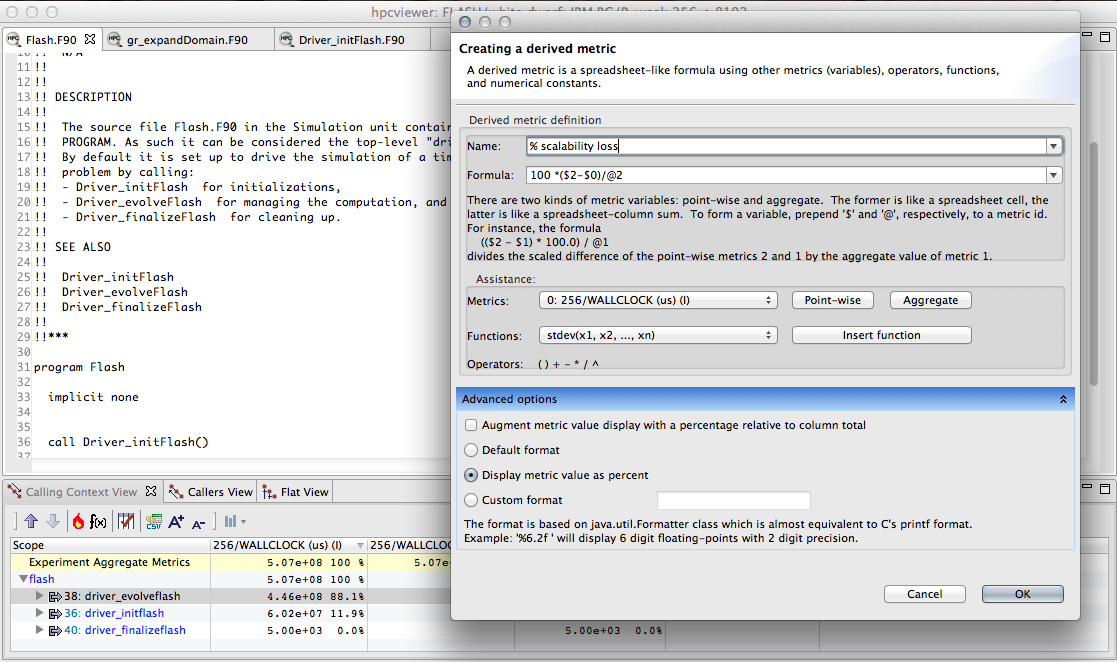
\includegraphics[width=1.0\textwidth]{fig/flash-scalability.png}}
%Two possible representations for the call path fragment $\ldots s_1 \rightarrow s_2 \ldots$, where $s_1$ and $s_2$ are call sites and where $s_1$ represents a call from $p$ to $q$ and $s_2$ a call from $q'$ to $r$.
\caption{Computing the scaling loss when weak scaling a white dwarf detonation simulation with FLASH3  from 256 to 8192 cores. For weak scaling, the time on an MPI rank in each of the simulations will be the same. In the figure, column 0 represents the inclusive cost for one MPI rank in a 256-core simulation; column 2 represents the inclusive cost for one MPI rank in an 8192-core simulation.  The difference between these two columns, computed as {\tt \$2-\$0},
represents the excess work present in the larger simulation for each unique program context in the calling context tree. Dividing that by the total time in the 8192-core execution {\tt @2} gives the fraction of wasted  time. Multiplying through by 100 gives the percent of the time wasted in the 8192-core execution, which corresponds to the \%~scalability loss.}
\label{fig:scaling-loss}
\end{figure}

\begin{figure}[t]
\center{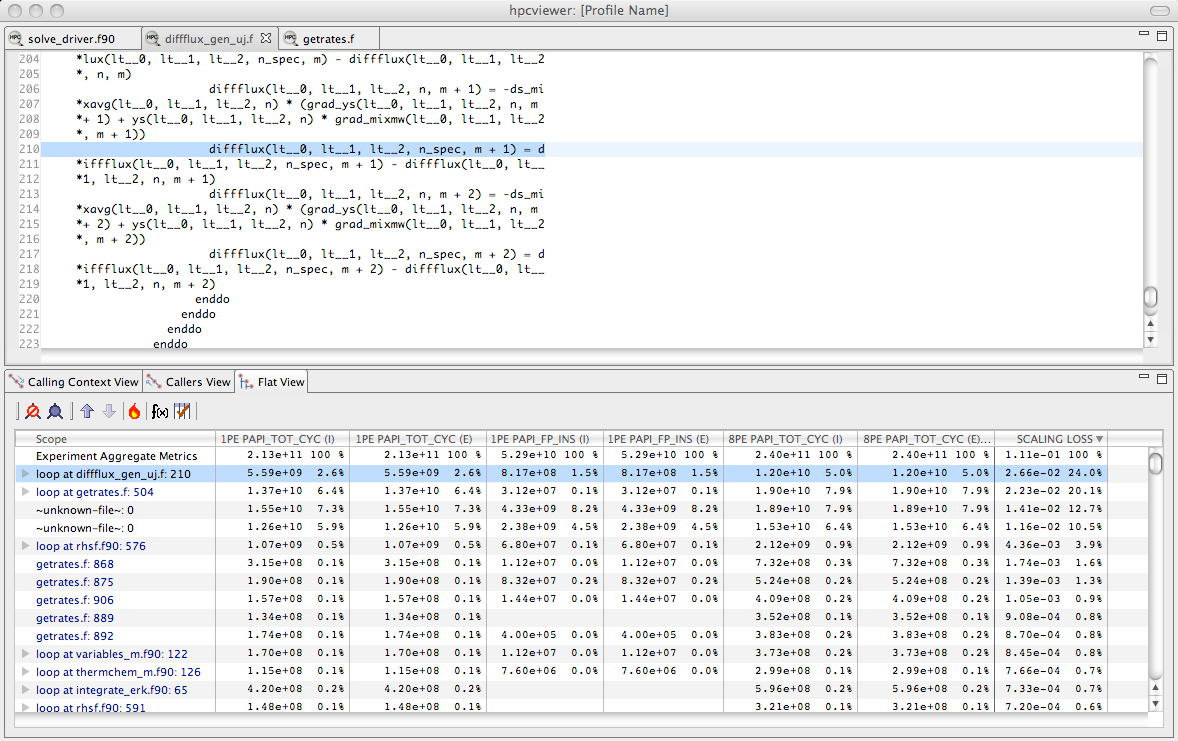
\includegraphics[width=1.0\textwidth]{fig/scaling-loss-2.png}}
%Two possible representations for the call path fragment $\ldots s_1 \rightarrow s_2 \ldots$, where $s_1$ and $s_2$ are call sites and where $s_1$ represents a call from $p$ to $q$ and $s_2$ a call from $q'$ to $r$.
\caption{Using the fraction the scalability loss metric of Figure~\ref{fig:scaling-loss} to rank order loop nests by their scaling loss.}
\label{fig:scaling-loss-2}
\end{figure}


\subsubsection*{Weak Scaling}

Consider two weak scaling experiments executed on $p$ and $q$ processors, respectively, $p<q$.
In Figure~\ref{fig:scaling-loss} shows how we can use a derived metric to compute and attribute scalability losses.
Here, we compute the difference in inclusive cycles spent on one core of a 8192-core run and one core in a 256-core run in a weak scaling experiment.
If the code had perfect weak scaling, the time for an MPI rank in each of the executions would be identical. In this case, they are not. 
We compute the excess work by computing the difference for each scope between the time on the 8192-core  run and the time on the 256-core core run. 
We normalize the differences of the time spent in the two runs by dividing then by the total time spent on the 8192-core  run. This yields the fraction of wasted effort 
for each scope when scaling from 256 to 8192 cores. Finally, we multiply these resuls by 100 to compute the \% scalability loss.
This example shows how one can compute a derived metric to that pinpoints and quantifies scaling losses across different node counts of a Blue Gene/P system.

A similar analysis can be applied to compute scaling losses between jobs that use different numbers of core counts on individual processors.
 Figure~\ref{fig:scaling-loss-2} shows the result of computing  the scaling loss for each loop nest when scaling from one to eight cores on a multicore node and rank order loop nests by their scaling loss metric. Here, we simply compute the scaling loss as the difference between the cycle counts of the eight-core and the one-core runs, divided through by the aggregate cost of the process executing on eight cores. This figure shows the scaling lost written in scientific notation as a fraction rather than multiplying through by 100 to yield a percent.
In this figure, we examine scaling losses in the flat view, showing them for each loop nest.
The source pane shows the loop nest responsible for the greatest scaling loss when scaling from one to eight cores.
Unsurprisingly, the loop with the worst scaling loss is very memory intensive.
Memory bandwidth is a precious commodity on multicore processors.

While we have shown how to compute and attribute the fraction of excess work in a weak scaling experiment, one can compute a similar quantity for experiments with strong scaling. When differencing the costs summed across all of the threads in a pair of strong-scaling experiments, one uses exactly the same approach as shown in Figure~\ref{fig:scaling-loss}. If comparing weak scaling costs summed across all ranks in $p$ and $q$ core executions, one can simply scale the aggregate costs by $1/p$ and $1/q$ respectively before differencing them. 


\subsubsection{Exploring Scaling Losses}

Scaling losses can be explored in \hpcviewer{} using any of its three views.

\begin{itemize}
\item {\em Top-down view.} This view represents the dynamic calling contexts (call paths) in which costs were incurred. 

\item {\em Bottom-up view.} This view enables one to look upward along call paths. This view is particularly useful for understanding the performance of software components or procedures that are used in more than one context, such as communication library routines.

\item {\em Flat view.} This view organizes performance measurement data according to the static structure of an application. All costs incurred in {\em any} calling context by a procedure are aggregated together in the flat view. 
\end{itemize}

\hpcviewer{} enables developers to explore top-down, bottom-up, and flat views of CCTs annotated with costs, helping to quickly pinpoint performance bottlenecks.
Typically, one begins analyzing an application's scalability and performance using the top-down calling context tree view.
Using this view, one can readily see how costs and scalability losses are associated with different calling contexts.
If costs or scalability losses are associated with only a few calling contexts, then this view suffices for identifying the bottlenecks.
When scalability losses are spread among many calling contexts, \eg, among different invocations of \mytt{MPI_Wait}, often it is useful to switch to the bottom-up of the data to see if many losses are due to the same underlying cause.
In the bottom-up view, one can sort routines by their exclusive scalability losses and then look upward to see how these losses accumulate from the different calling contexts in which the routine was invoked.

Scaling loss based on excess work is intuitive; perfect scaling corresponds to a excess work value of $0$, sublinear scaling yields positive values, and superlinear scaling yields negative values.
Typically, CCTs for SPMD programs have similar structure.
If CCTs for different executions diverge, using \hpcviewer{} to compute and report excess work will highlight these program regions.

Inclusive excess work and exclusive excess work serve as useful measures of scalability associated with nodes in a calling context tree (CCT).
By computing both metrics, one can determine whether the application scales well or not at a CCT node and also pinpoint the cause of any lack of scaling.
If a node for a function in the CCT has comparable positive values for both inclusive excess work and exclusive excess work, then the loss of scaling is due to computation in the function itself.
However, if the inclusive excess work for the function outweighs that accounted for by its exclusive costs, then one should explore the scalability of its callees.
To isolate code that is an impediment to scalable performance, one can use the {\em hot path} button in \hpcviewer{} to trace a path down through the CCT to see where the cost is incurred.


% ===========================================================================
% ===========================================================================

%\section{Identifying Load Imbalance}
%\label{sec:effective-performance-analysis:load-imbalance}


% ***************************************************************************
% ***************************************************************************

\chapter{Running Applications with \hpcrun{} and \hpclink{}}
\label{chpt:hpcrun}

%% $Id$

%%%%%%%%%%%%%%%%%%%%%%%%%%%%%%%%%%%%%%%%%%%%%%%%%%%%%%%%%%%%%%%%%%%%%%%%%%%%%
%%%%%%%%%%%%%%%%%%%%%%%%%%%%%%%%%%%%%%%%%%%%%%%%%%%%%%%%%%%%%%%%%%%%%%%%%%%%%

\documentclass[english]{article}
\usepackage[latin1]{inputenc}
\usepackage{babel}
\usepackage{verbatim}

%% do we have the `hyperref package?
\IfFileExists{hyperref.sty}{
   \usepackage[bookmarksopen,bookmarksnumbered]{hyperref}
}{}

%% do we have the `fancyhdr' or `fancyheadings' package?
\IfFileExists{fancyhdr.sty}{
\usepackage[fancyhdr]{latex2man}
}{
\IfFileExists{fancyheadings.sty}{
\usepackage[fancy]{latex2man}
}{
\usepackage[nofancy]{latex2man}
\message{no fancyhdr or fancyheadings package present, discard it}
}}

%% do we have the `rcsinfo' package?
\IfFileExists{rcsinfo.sty}{
\usepackage[nofancy]{rcsinfo}
\rcsInfo $Id$
\setDate{\rcsInfoLongDate}
}{
\setDate{ 2014/03/05}
\message{package rcsinfo not present, discard it}
}

\setVersionWord{Version:}  %%% that's the default, no need to set it.
\setVersion{=PACKAGE_VERSION=}

%%%%%%%%%%%%%%%%%%%%%%%%%%%%%%%%%%%%%%%%%%%%%%%%%%%%%%%%%%%%%%%%%%%%%%%%%%%%%
%%%%%%%%%%%%%%%%%%%%%%%%%%%%%%%%%%%%%%%%%%%%%%%%%%%%%%%%%%%%%%%%%%%%%%%%%%%%%

\begin{document}

\begin{Name}{1}{hpcrun}{The HPCToolkit Performance Tools}{The HPCToolkit Performance Tools}{hpcrun:\\ Statistical Profiling}

\Prog{hpcrun} is a call path profiler based on statistical sampling.
It supports multiple sample sources during one execution.
\Prog{hpcrun} profiles complex applications (forks, execs, threads and dynamic linking) and may be used in conjunction with parallel process launchers such as MPICH's \texttt{mpiexec} and SLURM's \texttt{srun}.

See \HTMLhref{hpctoolkit.html}{\Cmd{hpctoolkit}{1}} for an overview of \textbf{HPCToolkit}.


\end{Name}

%%%%%%%%%%%%%%%%%%%%%%%%%%%%%%%%%%%%%%%%%%%%%%%%%%%%%%%%%%%%%%%%%%
\section{Synopsis}

\Prog{hpcrun} \oOpt{profiling-options} \Arg{command} \oOpt{command-arguments}

\Prog{hpcrun} \oOpt{info-options}

%%%%%%%%%%%%%%%%%%%%%%%%%%%%%%%%%%%%%%%%%%%%%%%%%%%%%%%%%%%%%%%%%%
\section{Description}

\Prog{hpcrun} profiles the execution of an arbitrary command \Arg{command} using statistical sampling (rather than instrumentation).
It collects per-thread call path profiles that represent the full calling context of sample points.
Sample points may be generated from multiple simultaneous sampling sources.
\Prog{hpcrun} profiles complex applications that use forks, execs, threads, and dynamic linking/unlinking; it may be used in conjuction with parallel process launchers such as MPICH's \texttt{mpiexec} and SLURM's \texttt{srun}.

To profile a statically linked executable, make sure to link with \HTMLhref{hpclink.html}{\Cmd{hpclink}{1}}.

To configure \Prog{hpcrun}'s sampling sources, specify events and periods using the \texttt{-e/--event} option.
For an event \emph{e} and period \emph{p}, after every \emph{p} instances of \emph{e}, a sample is generated that causes \Prog{hpcrun} to inspect the and record information about the monitored \Arg{command}.

When \Arg{command} terminates, a profile measurement databse will be written to the directory:\\
\SP\SP\SP hpctoolkit-\Arg{command}-measurements[-\Arg{jobid}]\\
where \Arg{jobid} is a PBS or Sun Grid Engine job identifier.

\Prog{hpcrun} enables a user to abort a process and write the partial profiling data to disk by sending the Interrupt signal (INT or Ctrl-C).
This can be extremely useful on long-running or misbehaving applications.


%%%%%%%%%%%%%%%%%%%%%%%%%%%%%%%%%%%%%%%%%%%%%%%%%%%%%%%%%%%%%%%%%%
\section{Arguments}

\begin{Description}
\item[\Arg{command}] The command to profile.
\item[\Arg{command-arguments}] Arguments to the command to profile.
\end{Description}

Default values for an option's optional arguments are shown in \{\}.

\subsection{Options: Informational}

\begin{Description}
\item[\Opt{-l}, \Opt{-L}, \Opt{--list-events}]
List available events. (N.B.: some may not be profilable)

\item[\Opt{-V}, \Opt{--version}]
Print version information.

\item[\Opt{-h}, \Opt{--help}]
Print help.
\end{Description}

\subsection{Options: Profiling}

\begin{Description}

\item[\OptArg{-e}{event\Lbr@period\Rbr}, \OptArg{--event}{event\Lbr@period\Rbr}]
An event to profile and its corresponding sample period. \Arg{event} may be either a PAPI, native processor event, or WALLCLOCK (microseconds).  May pass multiple times as implementations permits.  \{\verb+WALLCLOCK@5000+\}
\begin{itemize}
  \item It is recommended to always specify the sampling period for each profiling event.
  \item The special event WALLCLOCK may be used to profile the `wall clock.'  It may be used only \emph{once} and cannot be used with another event. Its period is in microseconds.
  \item Hardware and drivers 1) limit the maximum number of events that can be monitored simultaneously, and 2) forbid certain combinations of events. 
  \item See the ``Sample sources'' under \textbf{NOTES} for additional details.
\end{itemize}

\item[\Opt{-t}, \Opt{--trace}]
Generate a call path trace (in addition to a call path profile).

\item[\OptArg{-f}{frac}, \OptArg{-fp}{frac}, \OptArg{--process-fraction}{frac}]
Measure only a fraction \Arg{frac} of the execution's processes.
For each process, enable measurement (of all threads) with probability \Arg{frac}; \Arg{frac} is a real number (0.10) or a fraction (1/10) between 0 and 1.
(To minimize perturbations, when a process is disabled, all threads in a process still receive sampling interrupts, but they are ignored.)

\item[\Opt{-r}, \Opt{--retain-recursion}]
Normally, hpcrun will collapse (simple) recursive call chains
to a single node. This option disables that behavior: all
elements of a recursive call chain are recorded
NOTE: If the user employs the RETCNT sample source, then this
      option is enabled: RETCNT implies *all* elements of
      call chains, including recursive elements, are recorded.



\item[\OptArg{-o}{outpath}, \OptArg{--output}{outpath}]
Directory for output data.
\{\verb+hpctoolkit-<command>-measurements[-<jobid>]+\}

\begin{itemize}
 Bug: Without a \Arg{jobid} or an output option, multiple profiles of the same <command> will be placed in the same output directory.
\end{itemize}

\end{Description}

%%%%%%%%%%%%%%%%%%%%%%%%%%%%%%%%%%%%%%%%%%%%%%%%%%%%%%%%%%%%%%%%%%

\section{Environment Variables}
For most systems, \Prog{hpcrun} requires no special environment variable settings.
There are two situations, however, where \Prog{hpcrun}, to function correctly,
\emph{must} refer to environment variables. These environment variables, and
corresponding situations are:
\begin{Description}
  \item[\verb+HPCTOOLKIT+] To function correctly, \Prog{hpcrun} must know
       the location of the \Prog{HPCToolkit} top-level installation directory.
       The \Prog{hpcrun} script uses elements of the installation \File{lib} and
       \File{libexec} subdirectories. For most systems, the 
       installation procedure ensures that \Prog{hpcrun} can find the requisite
       components. Some parallel job launchers, however, will \emph{copy} the
       \Prog{hpcrun} script to a different location from the installed base. If your
       system uses this copying mechanism, you must set the \verb+HPCTOOLKIT+
       environment variable to the top-level installation directory.
\end{Description}

%%%%%%%%%%%%%%%%%%%%%%%%%%%%%%%%%%%%%%%%%%%%%%%%%%%%%%%%%%%%%%%%%%

\section{Examples}

Assume we wish to profile the application \texttt{zoo}.
The following examples lists some useful events for different processor architectures.
In each case, the special option \texttt{--} is used to clearly demarcate the end of \Prog{hpcrun} options.

\begin{enumerate}
\item \verb+hpcrun -e WALLCLOCK@5000 zoo+

\item Opteron, (Rev B-F)
  \begin{enumerate}
    \item \verb+hpcrun -e DC_L2_REFILL@1300013 -e PAPI_L2_DCM@510011 -e PAPI_STL_ICY@5300013 -e PAPI_TOT_CYC@13000019 zoo+ (\verb+DC_L2_REFILL+ is an approximation of L1 D-cache misses).
    \item \verb+hpcrun -e PAPI_L2_DCM@510011 -e PAPI_TLB_DM@510013 -e PAPI_STL_ICY@5300013 -e PAPI_TOT_CYC@13000019 zoo+
  \end{enumerate}

\end{enumerate}

%%%%%%%%%%%%%%%%%%%%%%%%%%%%%%%%%%%%%%%%%%%%%%%%%%%%%%%%%%%%%%%%%%
\section{Notes}

\subsection{Sample sources}

\Prog{hpcrun} uses the PAPI library to provide access to hardware performance counter events.
If you have not configured HPCToolkit to use the PAPI library, you will be unable to measure hardware performance counter events.

The PAPI library supports a large collection of hardware counter events.
Some events have standard names across all platforms, e.g. \verb+PAPI_TOT_CYC+, the event that measures total cycles.
In addition to events whose names begin with the \verb+PAPI_+ prefix, platforms also provide access to a set of native events with names that are specific to the platform's processor.
A complete list of events supported by the PAPI library for your platform may be obtained by using the \texttt{--list-events} option.
Any event whose name begins with the \verb+PAPI_+ prefix that is listed as "Profilable" can be used as an event in a sampling source --- provided it does not conflict with another event.

The precise rules for selecting good events and periods are complex.
\begin{itemize}

\item \textbf{Choosing sampling events.}
We recommend using PAPI events in general.
However, some PAPI events are not profilable because of PAPI implementation details.
Also, PAPI's standard event list may not cover an architectural feature you are interested in.
In such cases, it is necessary to resort to native events.
In many cases, you will have to consult the architecture's manual to fully understand what the event means: there is no standard event list or naming scheme and events sometimes have unusual meanings.

\item \textbf{Number of sampling events.}
Currently, hpcrun does not multiplex hardware counters.
This means that the number of events that you may concurrently profile against is limited by your architecture's performance monitoring unit.
Note that some architectures hard-wire one or more counters to a specific event (such as cycles).

\item \textbf{Choosing sampling periods.}
The key requirement in choosing sampling periods is that you obtain enough samples to provide statistical significance.
We usually recommend a sampling rate between 100s-1000s of samples per second.
This usually only produces 1-5\% execution time overhead.

Choosing sampling rates depends on the architecture and sometimes the application.

Choosing periods for cycle and instruction-related events are usually easy.
Cycles directly relates to the clock speed.
Instruction-related events relates to the issue rate and width.

Choosing periods for other events seems harder because different applications uses resources differently.
For example, some applications are memory intensive and others are not.
However, if the goal is to identify rate-limiting factors of the architecture, then it is not necessary to consider the application.
For example, if the goal is to determine whether L2 D-cache latency is a limiting factor, then it is only necessary to work backward from the architecture's specifications to determine what number of L2 D-cache misses per second would be problematic.

\item \textbf{Architectural event conflicts.}
With some performance monitoring units, certain events may not be concurrently used with other events.

\item \textbf{Architectural interrupt delay.}
On most out-of-order pipelined architectures, a hardware counter interrupt is not precisely attributed to the instruction that induced the counter to overflow.
The gap is commonly 50-70 instructions.
This means that one should not assume that aggregation at the source line level is fully precise.
(E.g., if a L1 D-cache miss is attributed to a statement that has been compiled to register-only operations, assume the miss is attributed to a nearby load.)
However, aggregation at the procedure and loop level is reliable.

\item \textbf{System itimer (WALLCLOCK).}
On Linux systems, the kernel will not deliver itimer interrupts faster than the unit of a jiffy, which defaults to 4 milliseconds; see the itimer man page.
One can configure the kernel to use a value as small as 1 millisecond, but it is unlikely the kernel will actually deliver itimer signals at that rate when a period of 1000 microseconds is requested.

However, on Linux one can get quite close to the kernel Hz rate by setting the itimer interval to something less than the Hz rate.
For example, if the Hz rate is 1000 microseconds, one can use 500 microseconds (or just 1) and obtain about 999 interrupts per second.
\end{itemize}

\subsection{Platform-specific notes}
\subsubsection{Cray XE and XK}
When using dynamically linked binaries on Cray XE and XK systems, you
should add the \verb+HPCTOOLKIT+ environment variable to your launch
script.  Set \verb+HPCTOOLKIT+ to the top-level \verb+HPCToolkit+ install
prefix (the directory containing the \File{bin}, \File{lib} and
\File{libexec} subdirectories) and export it to the environment.  This is
only needed for running dynamically linked binaries.  For example:

\begin{verbatim}
#!/bin/sh
#PBS -l mppwidth=#nodes
#PBS -l walltime=00:30:00
#PBS -V

export HPCTOOLKIT=/path/to/hpctoolkit/install/directory

    ...Rest of Script...
\end{verbatim}

If \verb+HPCTOOLKIT+ is not set, you may see errors such as the
following in your job's error log.

\begin{verbatim}
/var/spool/alps/103526/hpcrun: Unable to find HPCTOOLKIT root directory.
Please set HPCTOOLKIT to the install prefix, either in this script,
or in your environment, and try again.
\end{verbatim}

The problem is that the Cray job launcher copies the \Prog{hpcrun}
script to a directory somewhere below \File{/var/spool/alps/} and runs
it from there.  By moving \Prog{hpcrun} to a different directory, this
breaks \Prog{hpcrun}'s method for finding its own install directory.
The solution is to add \verb+HPCTOOLKIT+ to your environment so that
\Prog{hpcrun} can find its install directory.

\subsection{Miscellaneous}

\begin{itemize}
  \item \Prog{hpcrun} uses preloaded shared libraries to initiate profiling.  For this reason, it cannot be used to profile setuid programs.
  \item \Prog{hpcrun} may not be able to profile programs that themselves use preloading.
\end{itemize}


%%%%%%%%%%%%%%%%%%%%%%%%%%%%%%%%%%%%%%%%%%%%%%%%%%%%%%%%%%%%%%%%%%
\section{See Also}

\HTMLhref{hpctoolkit.html}{\Cmd{hpctoolkit}{1}}.\\
\HTMLhref{hpclink.html}{\Cmd{hpclink}{1}}.


%%%%%%%%%%%%%%%%%%%%%%%%%%%%%%%%%%%%%%%%%%%%%%%%%%%%%%%%%%%%%%%%%%
\section{Version}

Version: \Version\ of \Date.

%%%%%%%%%%%%%%%%%%%%%%%%%%%%%%%%%%%%%%%%%%%%%%%%%%%%%%%%%%%%%%%%%%
\section{License and Copyright}

\begin{description}
\item[Copyright] \copyright\ 2002-2018, Rice University.
\item[License] See \File{README.License}.
\end{description}

%%%%%%%%%%%%%%%%%%%%%%%%%%%%%%%%%%%%%%%%%%%%%%%%%%%%%%%%%%%%%%%%%%
\section{Authors}

\noindent
Rice University's HPCToolkit Research Group \\
Email: \Email{hpctoolkit-forum =at= rice.edu} \\
WWW: \URL{http://hpctoolkit.org}.

\LatexManEnd

\end{document}

%% Local Variables:
%% eval: (add-hook 'write-file-hooks 'time-stamp)
%% time-stamp-start: "setDate{ "
%% time-stamp-format: "%:y/%02m/%02d"
%% time-stamp-end: "}\n"
%% time-stamp-line-limit: 50
%% End:




% ***************************************************************************
% ***************************************************************************

\chapter{Measurement and Analysis of GPU-accelerated Applications}
\label{chpt:gpu}

{
\centering
 \fbox{\parbox{\textwidth}{Note: This release contains beta support for monitoring computations offloaded onto  NVIDIA GPUs and alpha support for monitoring computations offloaded onto AMD GPUs.}}
 \vspace{2ex}
}


HPCToolkit can measure both the CPU and GPU performance of GPU-accelerated applications. It can measure CPU performance using asynchronous sampling triggered by Linux timers or hardware counter events as described in 
Section~\ref{sample-sources} and it can monitor GPU performance using tool support libraries provided by GPU vendors.

The foundation of HPCToolkit's support for measuring the performance of GPU-accelerated applications is a vendor-independent monitoring substrate. A thin software layer connects NVIDIA's CUPTI (CUDA Performance Tools Interface)~\cite{cupti} and AMD's ROC-tracer (ROCm Tracer Callback/Activity Library)~\cite{roctracer} monitoring libraries to this substrate. HPCToolkit reports GPU performance metrics in a vendor-neutral way. For instance, rather than focusing on NVIDIA warps or AMD wavefronts, HPCToolkit presents both as fine-grain, thread-level parallelism.

In the following sections, we describe how to use HPCToolkit to measure GPU metrics for GPU-accelerated applications. We begin with a discussion of NVIDIA GPUs since HPCToolkit's support for them is more complete than for others.

\begin{comment}

To measure both CUDA and OpenMP offloading performance, use one of the CUDA events specified above.
Postprocessing GPU Performance Measurements with HPCToolkit

Collecting Program Structure Information Using Binary Analysis
hpcstruct <load module>
Perform binary analysis to recover program structure of your executable or a shared library, as well as any NVIDIA CUBIN GPU binaries that are embedded in ELF segments. (Clang directly embeds NVIDIA CUBINs in ELF segments.)
hpcstruct hpctoolkit-<your application>-measurements
\end{comment}

\section{NVIDIA GPUs}

HPCToolkit supports two levels of performance monitoring for NVIDIA GPUs: coarse-grain profiling and tracing of GPU activities at the operation level (e.g., kernel launches, data allocations, memory copies, ...) , and fine-grain profiling of GPU computations using PC sampling, which measures GPU computations at a granularity of individual machine instructions. Section~\ref{nvidia-pc-sampling} describes fine-grain GPU performance measurement using PC sampling and the metrics it measures or computes. 

While performing coarse-grain GPU monitoring of kernel executions, memory copies, and other GPU activities, HPCToolkit will collect a trace of activity for each GPU stream if tracing is enabled. Table~\ref{nvidia-monitoring-options} shows the possible command-line arguments to \hpcrun{} that will enable different levels of monitoring  for NVIDIA GPUs. When fine-grain monitoring using PC sampling is enabled, coarse-grain profiling is also performed, so tracing is available in this mode as well.

Coarse-grain profiling attributes to each calling context the total time of all GPU operations initiated in that context. Table~\ref
{table:gtimes} shows the classes of GPU operations for which timings are collected. In addition, HPCToolkit records metrics for  operations performed including memory allocation and deallocation (Table~\ref{table:gmem}), memory set (Table~\ref{table:gmset}), explicit memory copies (Table~\ref{table:gxcopy}), and synchronization (Table~\ref{table:gsync}). In addition, HPCToolkit reports GPU kernel characteristics, including including register usage, as shown in Table~\ref{table:gker}.

\begin{table}[t]
\centering
\begin{tabular}{|l|p{3.5in}|}\hline
Argument to \hpcrun{} & What is monitored\\\hline\hline
{\tt -e gpu=nvidia} & profiling of GPU operations\\\hline
{\tt -e gpu=nvidia -t} & profiling and tracing of GPU operations\\\hline
{\tt -e gpu=nvidia,pc} &  PC sampling of GPU computations in addition to profiling of GPU operations\\\hline
{\tt -e gpu=nvidia,pc -t} &  PC sampling of GPU computations in addition to profiling and tracing of GPU operations\\\hline
\end{tabular}
\caption{Monitoring performance on NVIDIA GPUs.}
\label{nvidia-monitoring-options} 
\end{table}

\begin{table}[t]
\centering
\begin{tabular}{|l|l|}\hline
Metric & Description\\\hline\hline
 GKER (sec)  &  GPU time: kernel execution (seconds)  \\\hline 
  GMEM (sec)  &  GPU time: memory allocation/deallocation (seconds)  \\\hline 
  GMSET (sec)  &  GPU time: memory set (seconds)  \\\hline 
  GXCOPY (sec)  &  GPU time: explicit data copy (seconds)  \\\hline 
% GICOPY (sec)  &  GPU time: implicit data copy (seconds)  \\\hline 
  GSYNC (sec)  &  GPU time: synchronization (seconds)  \\\hline 
\end{tabular}
\caption{GPU operation timings.}
\label{table:gtimes}
\end{table}

\begin{table}[t]
\centering
\begin{tabular}{|l|l|}\hline
Metric & Description\\\hline\hline
 GMEM:UNK (B)  &  GPU memory alloc/free: unknown memory kind (bytes)  \\\hline
  GMEM:PAG (B)  &  GPU memory alloc/free: pageable memory (bytes)  \\\hline
  GMEM:PIN (B)  &  GPU memory alloc/free: pinned memory (bytes)  \\\hline
  GMEM:DEV (B)  &  GPU memory alloc/free: device memory (bytes)  \\\hline
  GMEM:ARY (B)  &  GPU memory alloc/free: array memory (bytes)  \\\hline
  GMEM:MAN (B)  &  GPU memory alloc/free: managed memory (bytes)  \\\hline
  GMEM:DST (B)  &  GPU memory alloc/free: device static memory (bytes)  \\\hline
  GMEM:MST (B)  &  GPU memory alloc/free: managed static memory (bytes)  \\\hline
  GMEM:COUNT  &  GPU memory alloc/free: count  \\\hline
\end{tabular}
\caption{GPU memory allocation and deallocation.}
\label{table:gmem}
\end{table}


\begin{table}[t]
\centering
\begin{tabular}{|l|l|}\hline
Metric & Description\\\hline\hline
 GMSET:UNK (B)  &  GPU memory set: unknown memory kind (bytes)  \\\hline
  GMSET:PAG (B)  &  GPU memory set: pageable memory (bytes)  \\\hline
  GMSET:PIN (B)  &  GPU memory set: pinned memory (bytes)  \\\hline
  GMSET:DEV (B)  &  GPU memory set: device memory (bytes)  \\\hline
  GMSET:ARY (B)  &  GPU memory set: array memory (bytes)  \\\hline
  GMSET:MAN (B)  &  GPU memory set: managed memory (bytes)  \\\hline
  GMSET:DST (B)  &  GPU memory set: device static memory (bytes)  \\\hline
  GMSET:MST (B)  &  GPU memory set: managed static memory (bytes)  \\\hline
  GMSET:COUNT  &  GPU memory set: count  \\\hline
\end{tabular}
\caption{GPU memory set metrics.}
\label{table:gmset}
\end{table}

\begin{table}[t]
\centering
\begin{tabular}{|l|l|}\hline
Metric & Description\\\hline\hline
 GXCOPY:UNK (B)  &  GPU explicit memory copy: unknown kind (bytes)  \\\hline 
  GXCOPY:H2D (B)  &  GPU explicit memory copy: host to device (bytes)  \\\hline 
  GXCOPY:D2H (B)  &  GPU explicit memory copy: device to host (bytes)  \\\hline 
  GXCOPY:H2A (B)  &  GPU explicit memory copy: host to array (bytes)  \\\hline 
  GXCOPY:A2H (B)  &  GPU explicit memory copy: array to host (bytes)  \\\hline 
  GXCOPY:A2A (B)  &  GPU explicit memory copy: array to array (bytes)  \\\hline 
  GXCOPY:A2D (B)  &  GPU explicit memory copy: array to device (bytes)  \\\hline 
  GXCOPY:D2A (B)  &  GPU explicit memory copy: device to array (bytes)  \\\hline 
  GXCOPY:D2D (B)  &  GPU explicit memory copy: device to device (bytes)  \\\hline 
  GXCOPY:H2H (B)  &  GPU explicit memory copy: host to host (bytes)  \\\hline 
  GXCOPY:P2P (B)  &  GPU explicit memory copy: peer to peer (bytes)  \\\hline 
  GXCOPY:COUNT  &  GPU explicit memory copy: count  \\\hline 
\end{tabular}
\caption{GPU explicit memory copy metrics.}
\label{table:gxcopy}
\end{table}


\begin{table}[h]
\centering
\begin{tabular}{|l|l|}\hline
Metric & Description\\\hline\hline
 GSYNC:UNK (us)  &  GPU synchronizations: unknown kind  \\\hline 
  GSYNC:EVT (us)  &  GPU synchronizations: event  \\\hline 
  GSYNC:STRE (us)  &  GPU synchronizations: stream event wait  \\\hline 
  GSYNC:STR (us)  &  GPU synchronizations: stream  \\\hline 
  GSYNC:CTX (us)  &  GPU synchronizations: context  \\\hline 
  GSYNC:COUNT  &  GPU synchronizations: count  \\\hline 
\end{tabular}
\caption{GPU synchronization metrics.}
\label{table:gsync}
\end{table}


\begin{table}[h]
\centering
\begin{tabular}{|l|l|}\hline
Metric & Description\\\hline\hline
GKER:STMEM (B) & GPU kernel: static memory (bytes)    \\\hline
GKER:DYMEM (B) & GPU kernel: dynamic memory (bytes)   \\\hline
GKER:LMEM (B) & GPU kernel: local memory (bytes)    \\\hline
GKER:FGP\_ACT & GPU kernel: fine-grain parallelism, actual    \\\hline
GKER:FGP\_MAX & GPU kernel: fine-grain parallelism, maximum    \\\hline
GKER:THR\_REG & GPU kernel: thread register count    \\\hline
GKER:BLK\_THR & GPU kernel: thread count   \\\hline
GKER:BLK\_SM (B) & GPU kernel: block local memory (bytes)   \\\hline
GKER:COUNT & GPU kernel: launch count   \\\hline
GKER:OCC & GPU kernel: occupancy    \\\hline
\end{tabular}
\caption{GPU kernel characteristic metrics.}
\label{table:gker}
\end{table}

\begin{comment}
\begin{table}
\centering
\begin{tabular}{|l|p{3.5in}|}\hline
Metric & Description\\\hline\hline
 GGMEM:LDC (B)  &  GPU global memory: load cacheable memory (bytes)  \\\hline 
  GGMEM:LDU (B)  &  GPU global memory: load uncacheable memory (bytes)  \\\hline 
  GGMEM:ST (B)  &  GPU global memory: store (bytes)  \\\hline 
  GGMEM:LDC (L2T)  &  GPU global memory: load cacheable (L2 cache transactions)  \\\hline 
  GGMEM:LDU (L2T)  &  GPU global memory: load uncacheable (L2 cache transactions)  \\\hline 
  GGMEM:ST (L2T)  &  GPU global memory: store (L2 cache transactions)  \\\hline 
  GGMEM:LDCT (L2T)  &  GPU global memory: load cacheable    (L2 cache transactions, theoretical)  \\\hline 
  GGMEM:LDUT (L2T)  &  GPU global memory: load uncacheable    (L2 cache transactions, theoretical)  \\\hline 
  GGMEM:STT (L2T)  &  GPU global memory: store    (L2 cache transactions, theoretical)  \\\hline 
\end{tabular}
\caption{GPU global memory metrics.}
\label{table:ggmem}
\end{table}


\begin{table}
\centering
\begin{tabular}{|l|l|}\hline
Metric & Description\\\hline\hline
 GLMEM:LD (B)  &  GPU local memory: load (bytes)  \\\hline 
  GLMEM:ST (B)  &  GPU local memory: store (bytes)  \\\hline 
  GLMEM:LD (T)  &  GPU local memory: load (transactions)  \\\hline 
  GLMEM:ST (T)  &  GPU local memory: store (transactions)  \\\hline 
  GLMEM:LDT (T)  &  GPU local memory: load (transactions, theoretical)  \\\hline 
  GLMEM:STT (T)  &  GPU local memory: store (transactions, theoretical)  \\\hline 
\end{tabular}
\caption{GPU local memory metrics.}
\label{table:gmem}
\end{table}



\begin{table}
\centering
\begin{tabular}{|l|p{3.5in}|}\hline
Metric & Description\\\hline\hline
 GICOPY:UNK (B)  &  GPU implicit copy: unknown kind (bytes)  \\\hline 
  GICOPY:H2D (B)  &  GPU implicit copy: host to device (bytes)  \\\hline 
  GICOPY:D2H (B)  &  GPU implicit copy: device to host (bytes)  \\\hline 
  GICOPY:D2D (B)  &  GPU implicit copy: device to device (bytes)  \\\hline 
  GICOPY:CPU\_PF  &  GPU implicit copy: CPU page faults  \\\hline 
  GICOPY:GPU\_PF  &  GPU implicit copy: GPU page faults  \\\hline 
  GICOPY:THRASH  &  GPU implicit copy: CPU thrashing page faults    (data frequently migrating between processors)  \\\hline 
  GICOPY:THROT  &  GPU implicit copy: throttling    (prevent thrashing by delaying page fault service)  \\\hline 
  GICOPY:RMAP  &  GPU implicit copy: remote maps    (prevent thrashing by pinning memory for a time with    some processor mapping and accessing it remotely)  \\\hline 
  GICOPY:COUNT  &  GPU implicit copy: count  \\\hline 
\end{tabular}
\caption{GPU implicit memory copy metrics.}
\label{table:gtimes}
\end{table}


\begin{table}
\centering
\begin{tabular}{|l|l|}\hline
Metric & Description\\\hline\hline
 GBR:DIV  &  GPU branches: diverged  \\\hline 
  GBR:EXE  &  GPU branches: executed  \\\hline 
\end{tabular}
\caption{GPU branch metrics.}
\label{table:gbr}
\end{table}
\end{comment}


At present, using NVIDIA's CUPTI library adds substantial measurement overhead.  Unlike CPU monitoring based on asynchronous sampling, GPU performance monitoring uses vendor-provided callback interfaces to intercept the initiation of each GPU operation. Accordingly,  the overhead of GPU performance monitoring depends upon how frequently GPU operations are initiated. 
In our experience to date, profiling (and if requested, tracing) on NVIDIA GPUs using NVIDIA's CUPTI interface roughly doubles the execution time of a GPU-accelerated application. In our experience, we have seen NVIDIA's PC sampling dilate the execution time of a GPU-accelerated program by $30\times$. The overhead of GPU monitoring is principally on the host side. As measured by CUPTI, the time spent in GPU operations or PC samples are expected to be relatively accurate. However, since execution as a whole is slowed while measuring GPU performance, when evaluating GPU activity reported by HPCToolkit, one must be careful.

For instance, if a GPU-accelerated program runs in 1000 seconds without HPCToolkit monitoring GPU activity but slows to 2000 seconds when GPU profiling and tracing is enabled, then if GPU profiles and traces show that the GPU is active for 25\% of the execution time, one should  re-scale the accurate measurements of GPU activity by considering the $2\times$ dilation when monitoring GPU activity. Without monitoring, one would expect the same level of GPU activity, but the host time would be twice as fast. Thus, without monitoring, the ratio of GPU activity to host activity would be roughly double.
 

\subsection{PC Sampling on NVIDIA GPUs}
\label{nvidia-pc-sampling} 

NVIDIA's GPUs have supported PC sampling since Maxwell~\cite{cuptipcsampling}.
Instruction samples are collected separately on each active streaming
multiprocessor (SM) and merged in a buffer returned by NVIDIA's CUPTI. 
In each sampling period, one warp scheduler of each active SM 
samples the next instruction from one of its active warps. Sampling rotates through
an SM's warp schedulers in a round robin fashion.
When an instruction is sampled, its stall reason (if any) is
recorded. If all warps on a scheduler are stalled when a sample is
taken, the sample is marked as a latency sample, meaning no instruction will be issued by the warp scheduler in the next cycle.
Figure~\ref{fig:pc sampling} shows a PC sampling example on an SM with four schedulers. Among the six collected samples, four are latency samples, so the estimated stall ratio is $4/6$. 

Figure~\ref{table:pc-stall} shows the stall metrics recorded by HPCToolkit using CUPTI's PC sampling. Figure~\ref{table:gsamp} shows PC sampling summary statistics recorded by HPCToolkit. Of particular note is the metric \verb|GSAMP:UTIL|. HPCToolkit computes approximate GPU utilization using information gathered using PC sampling. Given the average clock frequency and the sampling rate, if all SMs are active, then HPCToolkit knows how many instruction samples would be expected ({\tt GSAMP:EXP}) if the GPU was fully active for the interval when it was in use. HPCToolkit approximates the percentage of GPU utilization by comparing the measured samples with the expected samples using the following formula: $100 * {\tt (GSAMP:TOT)/ (GSAMP:EXP)}$.


\begin{figure}[t]
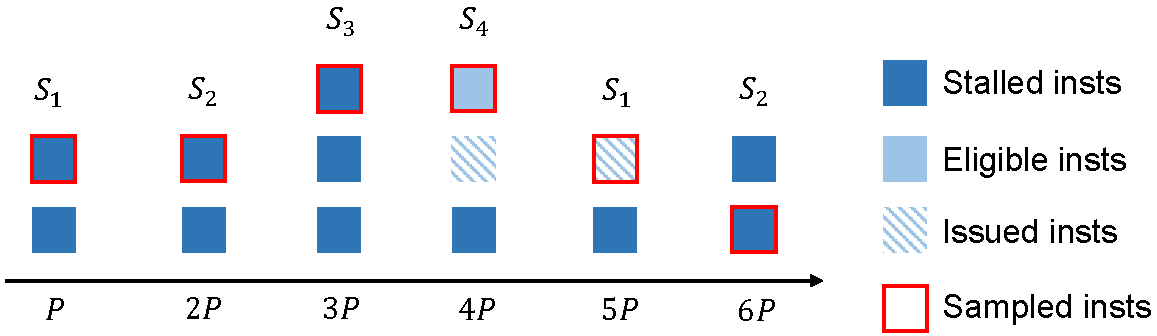
\includegraphics[width=\textwidth]{mental-model.pdf}
\caption{NVIDIA's GPU PC sampling example on an SM. $P-6P$ represent
six sample periods P cycles apart. $S_{1}-S_{4}$ represent four schedulers on an SM.}
\label{fig:pc sampling}
\vspace{-2ex}
\end{figure}

\begin{table}[t]
\centering
\begin{tabular}{|l|p{3.5in}|}\hline
Metric & Description\\\hline\hline
GINST & GPU instructions executed\\\hline
GINST:STL\_ANY  &  GPU instruction stalls: any  \\\hline 
 GINST:STL\_NONE  &  GPU instruction stalls: no stall  \\\hline 
 GINST:STL\_IFET  &  GPU instruction stalls: await availability of next    instruction (fetch or branch delay)  \\\hline 
 GINST:STL\_IDEP  &  GPU instruction stalls: await satisfaction of instruction    input dependence  \\\hline 
 GINST:STL\_GMEM  &  GPU instruction stalls: await completion of global memory    access  \\\hline 
 GINST:STL\_TMEM  &  GPU instruction stalls: texture memory request queue full  \\\hline 
 GINST:STL\_SYNC  &  GPU instruction stalls: await completion of thread or    memory synchronization  \\\hline 
 GINST:STL\_CMEM  &  GPU instruction stalls: await completion of constant or    immediate memory access  \\\hline 
 GINST:STL\_PIPE  &  GPU instruction stalls: await completion of required    compute resources  \\\hline 
 GINST:STL\_MTHR  &  GPU instruction stalls: global memory request queue full  \\\hline 
 GINST:STL\_NSEL  &  GPU instruction stalls: not selected for issue but ready  \\\hline 
 GINST:STL\_OTHR  &  GPU instruction stalls: other  \\\hline 
 GINST:STL\_SLP  &  GPU instruction stalls: sleep  \\\hline 
\end{tabular}
\caption{GPU instruction execution and stall metrics.}
\label{table:pc-stall}
\end{table}

\begin{table}[t]
\centering
\begin{tabular}{|l|l|}\hline
Metric & Description\\\hline\hline
 GSAMP:DRP  &  GPU PC samples: dropped  \\\hline 
  GSAMP:EXP  &  GPU PC samples: expected  \\\hline 
  GSAMP:TOT  &  GPU PC samples: measured  \\\hline 
  GSAMP:PER (cyc)  &  GPU PC samples: period (GPU cycles)  \\\hline 
  GSAMP:UTIL (\%) & GPU utilization computed using PC sampling\\\hline
\end{tabular}
\caption{GPU PC sampling statistics.}
\label{table:gsamp}
\end{table}



For CUDA 10, measurement using PC sampling with CUPTI serializes the execution of GPU kernels. Thus, measurement of GPU kernels using PC sampling will distort the execution of a GPU-accelerated application by blocking concurrent execution of GPU kernels. For applications that rely on concurrent kernel execution to keep the GPU busy, this will significantly distort execution and PC sampling measurements will only reflect the GPU activity of kernels running in isolation.




\subsection{Attributing Measurements to Source Code for NVIDIA GPUs}

NVIDIA's {\tt nvcc} compiler doesn't record information about how GPU machine code maps to CUDA source without proper compiler arguments. Using the {\tt -G} compiler option to {\tt nvcc}, one may generate NVIDIA CUBINs with full DWARF information that includes not only line maps, which map each machine instruction back to a program source line, but also detailed information about inlined code. However, the price of turning on {\tt -G} is that optimization by {\tt nvcc} will be disabled. For that reason, the performance of code compiled {\tt -G} is vastly slower. While a developer of a template-based programming model may find this option useful to see how a program employs templates to instantiate GPU code, measurements of code compiled with {\tt -G} should be viewed with skeptical eye.

One can use {\tt nvcc}'s {\tt -lineinfo } option to instruct {\tt nvcc} to record line map information during compilation.\footnote{Line maps relate each machine instruction back to the program source line from where it came.} The {\tt -lineinfo} option can be used in conjunction with {\tt nvcc} optimization. Using {\tt -lineinfo}, one can measure and interpret the performance of optimized code. However, line map information is a poor substitute for full DWARF information. When {\tt nvcc} inlines code during optimization, the resulting line map information simply shows that source lines that were compiled into a GPU function. A developer examining performance measurements for a function must reason on their own about how any source lines from outside the function got there as the result of inlining and/or macro expansion.

When HPCToolkit uses NVIDIA's CUPTI to monitor a GPU-accelerated application, 
CUPTI notifies HPCToolkit every time it loads a CUDA binary, known as a CUBIN, into a GPU.
At runtime, HPCToolkit computes a cryptographic hash of a CUBIN's contents and records the CUBIN into the execution's measurement directory. 
For instance, if a GPU-accelerated application loaded CUBIN into a GPU, NVIDIA's CUPTI informed HPCToolkit that the CUBIN was being loaded, and HPCToolkit computed its cryptographic hash as {\tt 972349aed8}, then HPCToolkit would record {\tt 972349aed8.cubin} inside a {\tt cubins} subdirectory of an HPCToolkit measurement directory. 

To  attribute GPU performance measurements back to source, HPCToolkit's \hpcstruct{} supports analysis of NVIDIA CUBIN binaries. Since many CUBIN binaries may be loaded  by a GPU-accelerated application during execution,  an application's measurements directory may contain a {\tt cubins} subdirectory populated with many CUBINs. In this case, it would be inconvenient to require a developer to apply \hpcstruct{} manually to analyze each CUBIN. To simplify the analysis of an execution's CUBINs, a developer may apply HPCToolkit's \hpcstruct{} directly to a measurement directory to analyze all of the CUBINs it contains. Namely, for a measurements directory {\tt hpctoolkit-laghos-measurements} collected during an execution of the GPU-accelerated laghos mini-app~\cite{laghos}, one can analyze all of the CUBINs collected during execution by using the following command:

\begin{quote}
\begin{verbatim}
hpcstruct hpctoolkit-laghos-measurements
\end{verbatim}
\end{quote}


Since there may be many CUBINs inside an HPCToolkit measurements directory for a GPU-accelerated application, it is useful to accelerate the analysis of an execution's CUBINs by employing parallelism. One can analyze the set of CUBINs in an HPCToolkit measurements directory by using \hpcstruct's {\tt -j} option. For instance, one can use 16 threads to analyze the CUBINs in the {\tt hpctoolkit-laghos-measurements} directory with the following command:

\begin{quote}
\begin{verbatim}
hpcstruct -j 16 hpctoolkit-laghos-measurements
\end{verbatim}
\end{quote}

By default, when applied to a measurements directory, \hpcstruct{} performs only lightweight analysis of the GPU functions in each CUBIN. When a measurements directory contains fine-grain measurements collected using PC sampling, it is useful to perform a more detailed analysis to recover information about the loops and call sites of GPU functions in an NVIDIA CUBIN. Unfortunately, NVIDIA has refused to provide an API that would enable HPCToolkit to perform instruction-level analysis of CUBINs directly. Instead, HPCToolkit must invoke NVIDIA's {\tt nvdisasm} command line utility to compute control flow graphs for functions in a CUBIN. The version of {\tt nvdisasm} in CUDA 10 is slow and fails to compute control flow graphs for some GPU functions. In such cases, \hpcstruct{} reverts to lightweight analysis of GPU functions that considers only line map information. Because analysis of CUBINs using {\tt nvdisasm} is slow, it is not performed by default. To enable detailed analysis of GPU functions, use the {\tt --gpucfg yes} option to \hpcstruct{}, as shown below:

\begin{quote}
\begin{verbatim}
hpcstruct -j 16 --gpucfg yes hpctoolkit-laghos-measurements
\end{verbatim}
\end{quote}


\subsection{GPU Calling Context Tree Reconstruction}
\label{nvidia-cct}



The CUPTI API returns flat PC samples without any information about GPU call stacks.
With complex code generated from template-based GPU programming models, calling contexts on GPUs are essential for developers to understand the code and its performance. Lawrence Livermore National Laboratory's GPU-accelerated Quicksilver proxy app~\cite{quicksilver} illustrates this problem. Figure~\ref{qs-no-cct} shows a \hpcviewer{} screenshot of Quicksilver without approximate reconstruction the GPU calling context tree. The figure shows a top-down view of heterogeneous calling contexts that span both the CPU and GPU. In the middle of the figure is a placeholder \verb|<gpu kernel>| that is inserted by HPCToolkit. Above the placeholder is a CPU calling context where a GPU kernel was invoked. Below the \verb|<gpu kernel>| placeholder, \hpcviewer{} shows a dozen of the GPU functions that were executed on behalf of the GPU kernel \verb|CycleTrackingKernel|. 

\begin{figure}[t]
\centering
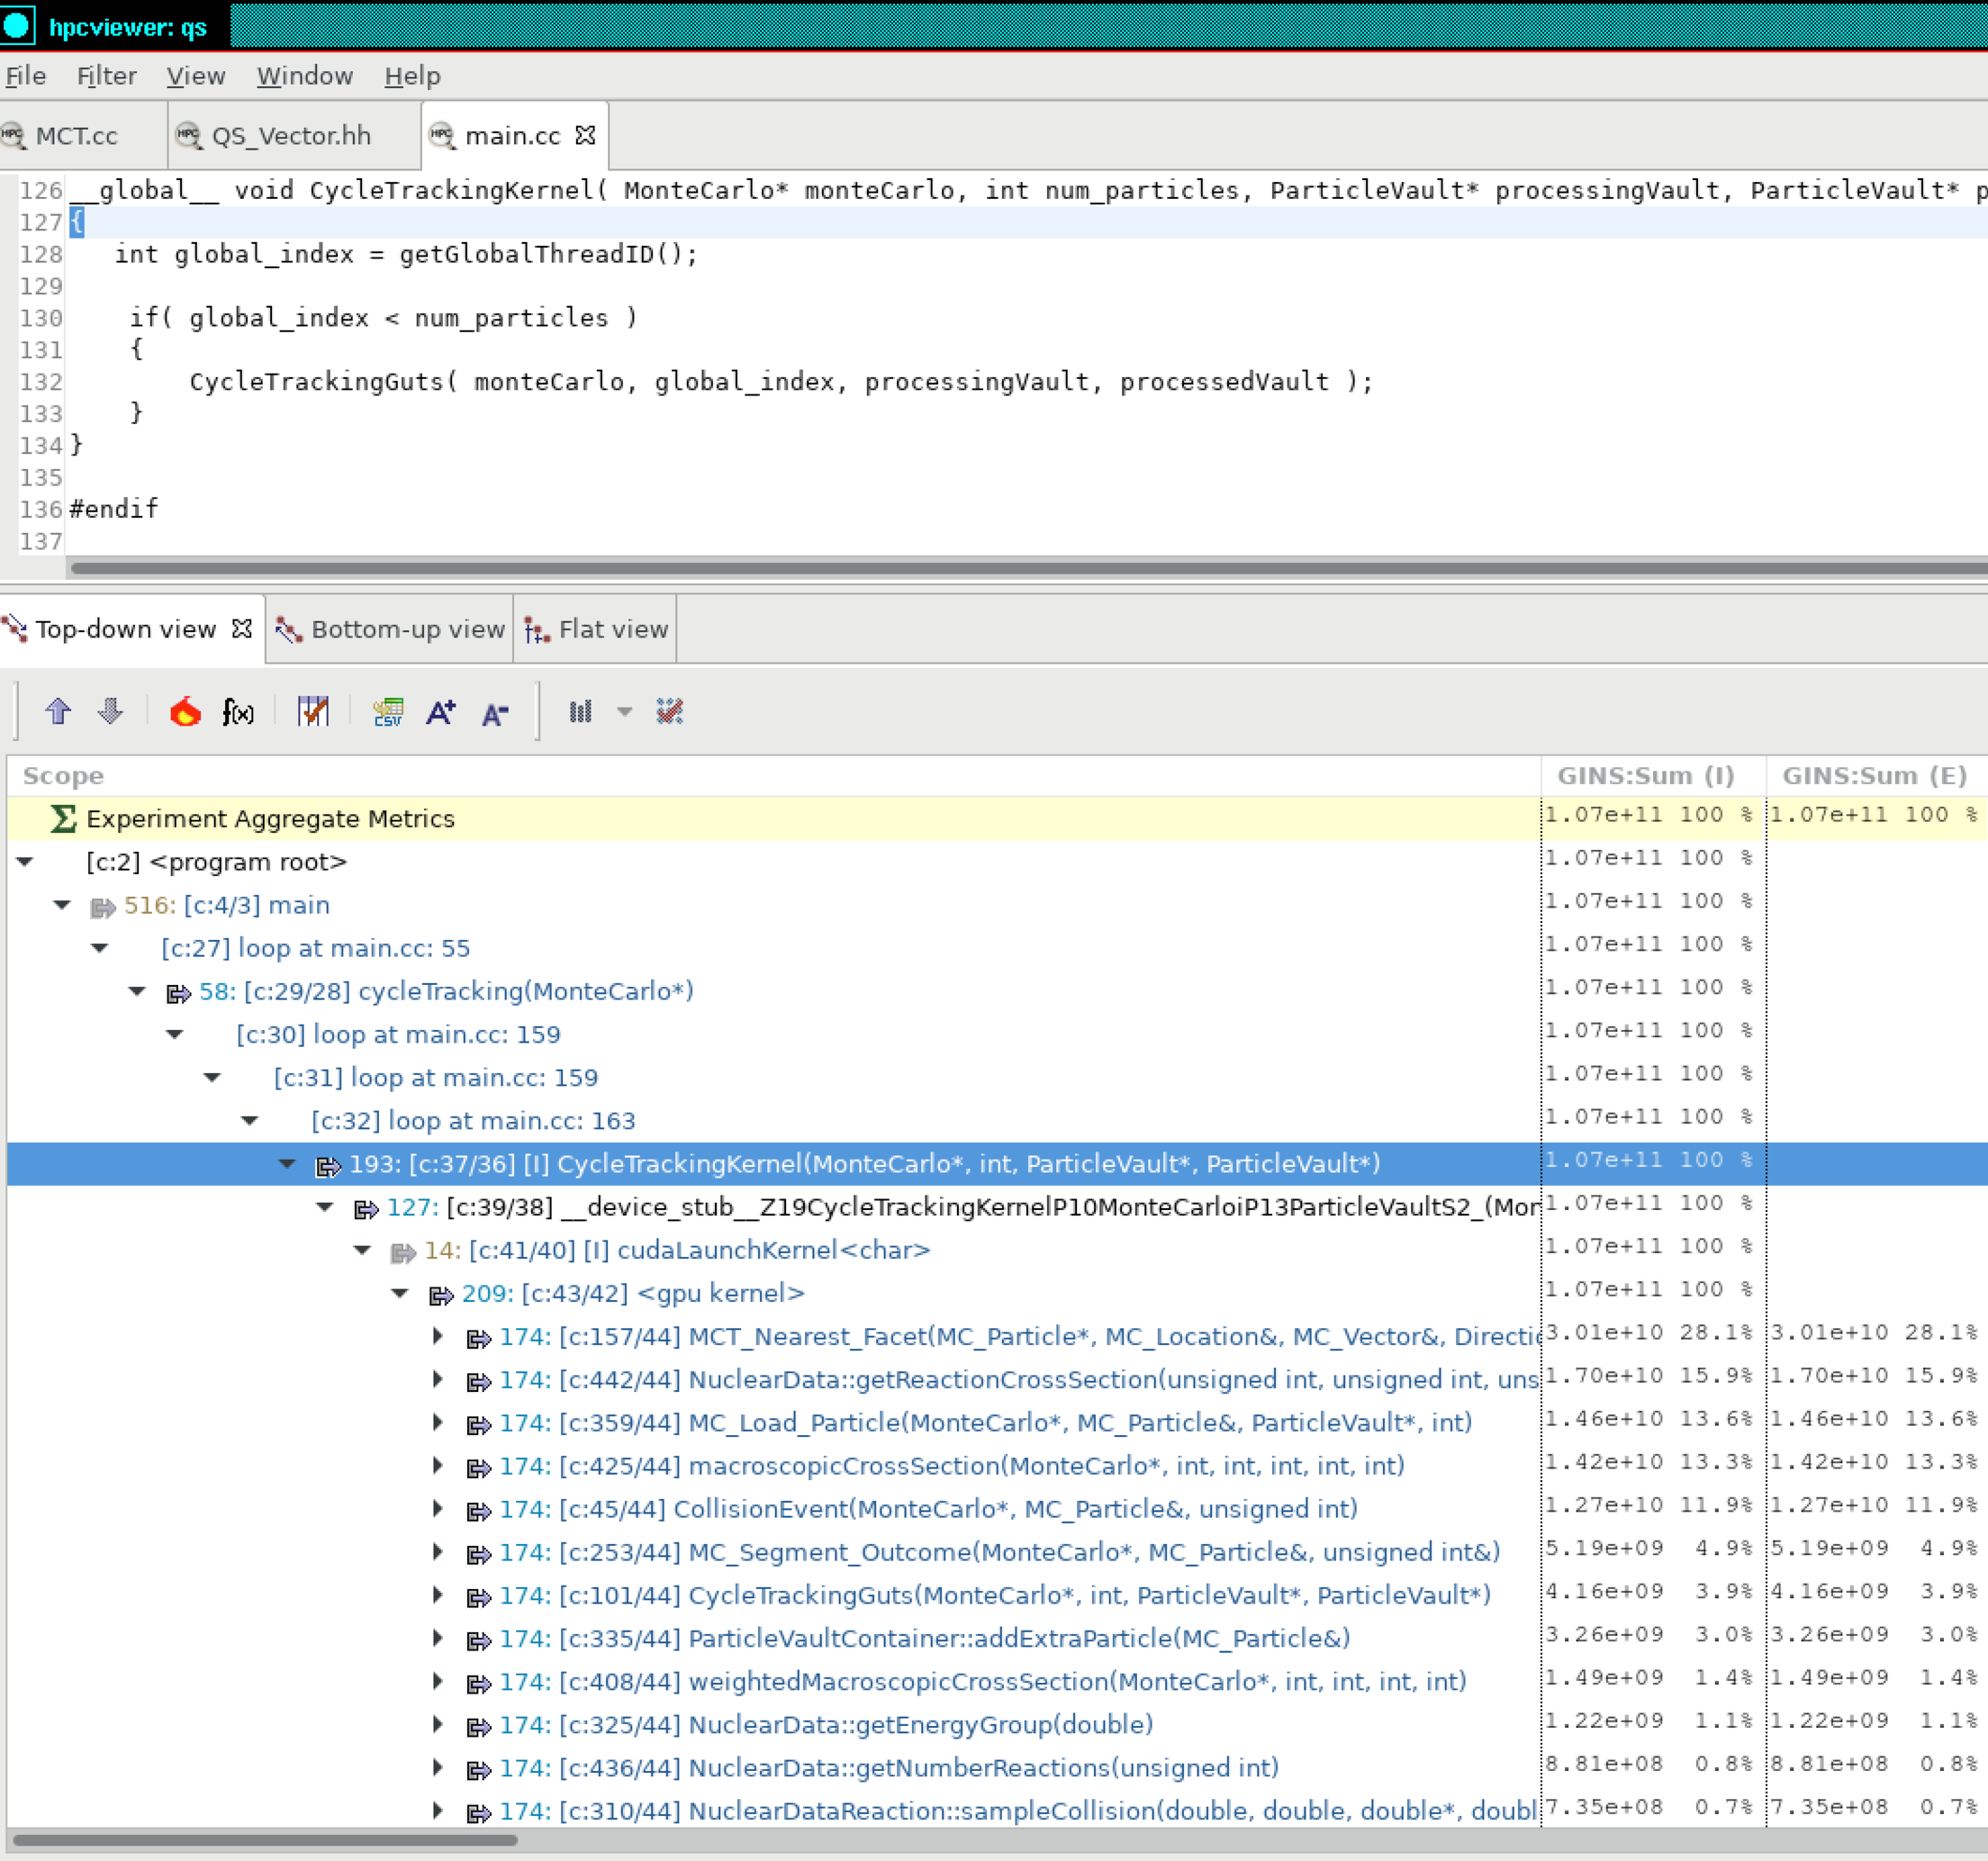
\includegraphics[width=\textwidth]{qs-no-cct.pdf}
\caption{A screenshot of \hpcviewer{} for the GPU-accelerated Quicksilver proxy app without GPU CCT reconstruction.}
\label{qs-no-cct}
\end{figure}


Currently, no API is available for efficiently unwinding call stacks on NVIDIA's GPUs.
To address this issue, we designed a method to reconstruct approximate GPU calling contexts using post-mortem analysis. This analysis is only performed when (1) an execution has been monitored using PC sampling, and (2) an execution's CUBINs have analyzed in detail using \hpcstruct{} with the {\tt --gpucfg yes} option.

To reconstruct approximate calling context trees for GPU computations, HPCToolkit uses information about call sites identified by \hpcstruct{} in conjunction with PC samples measured for each {\tt call} instruction in GPU binaries. 

Without the ability to measure each function invocation in detail, HPCToolkit assumes that each invocation of a particular GPU function incurs the same costs. The costs of each GPU function are apportioned among its caller or callers using the following rules:

\begin{itemize}
\item
If a GPU function G can only be invoked from a single call site, all of the measured cost of G will be attributed to its call site. 
\item
If a GPU function G can be called from multiple call sites and PC samples have been collected for one or more of the call instructions for G, the costs for G are proportionally divided among G's call sites according to the distribution of PC samples for calls that invoke G.  For instance, consider the case where there are three call sites where G may be invoked, 5 samples are recorded for the first call instruction, 10 samples are recorded for the second call instruction, and no samples are recorded for the third call. In this case, HPCToolkit divides the costs for G  among the first two call sites, attributing $5/15$ of G's costs  to the first call site and $10/15$ of G's costs to the second call site. 
\item
If no call instructions for a GPU function G have been sampled, the costs of G are apportioned evenly among each of G's call sites.
\end{itemize}

IHPCToolkit's {\tt hpcprof} analyzes the static call graph associated with each GPU kernel invocation. If the static call graph for the GPU kernel contains cycles, which arise from recursive or mutually-recursive calls,  \hpcprof{} replaces each cycle with a strongly connected component (SCC). In this case, \hpcprof{} unlink's call graph edges between vertices within the SCC and adds an SCC vertex to enclose the set of vertices in each SCC. The rest of \hpcprof{}'s analysis 
treats an SCC vertex as a normal ``function'' in the call graph.

\begin{figure}[t]
\centering
\begin{subfigure}{0.22\textwidth}
\centering
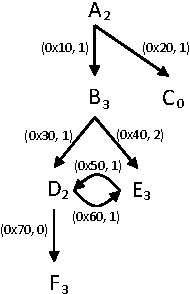
\includegraphics[width=0.6\textwidth]{cct-1.pdf}
\caption{}
\end{subfigure}
~
\begin{subfigure}{0.22\textwidth}
\centering
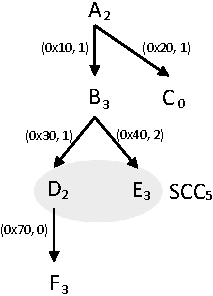
\includegraphics[width=0.6\textwidth]{cct-2.pdf}
\caption{}
\end{subfigure}
~
\begin{subfigure}{0.22\textwidth}
\centering
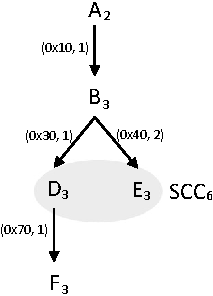
\includegraphics[width=0.6\textwidth]{cct-3.pdf}
\caption{}
\end{subfigure}
~
\begin{subfigure}{0.22\textwidth}
\centering
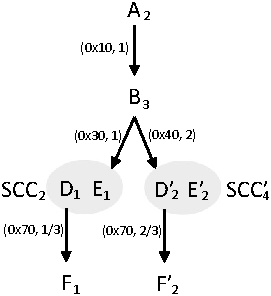
\includegraphics[width=0.8\textwidth]{cct-4.pdf}
\caption{}
\end{subfigure}
\caption{Reconstruct a GPU calling context tree. A-F represent GPU functions. Each subscript denotes the number of samples associated with the function. Each $(a, c)$ pair indicates an edge at address $a$ has $c$ call instruction samples.}
\label{fig:gpu calling context tree}
\end{figure}

\begin{figure}[t]
\centering
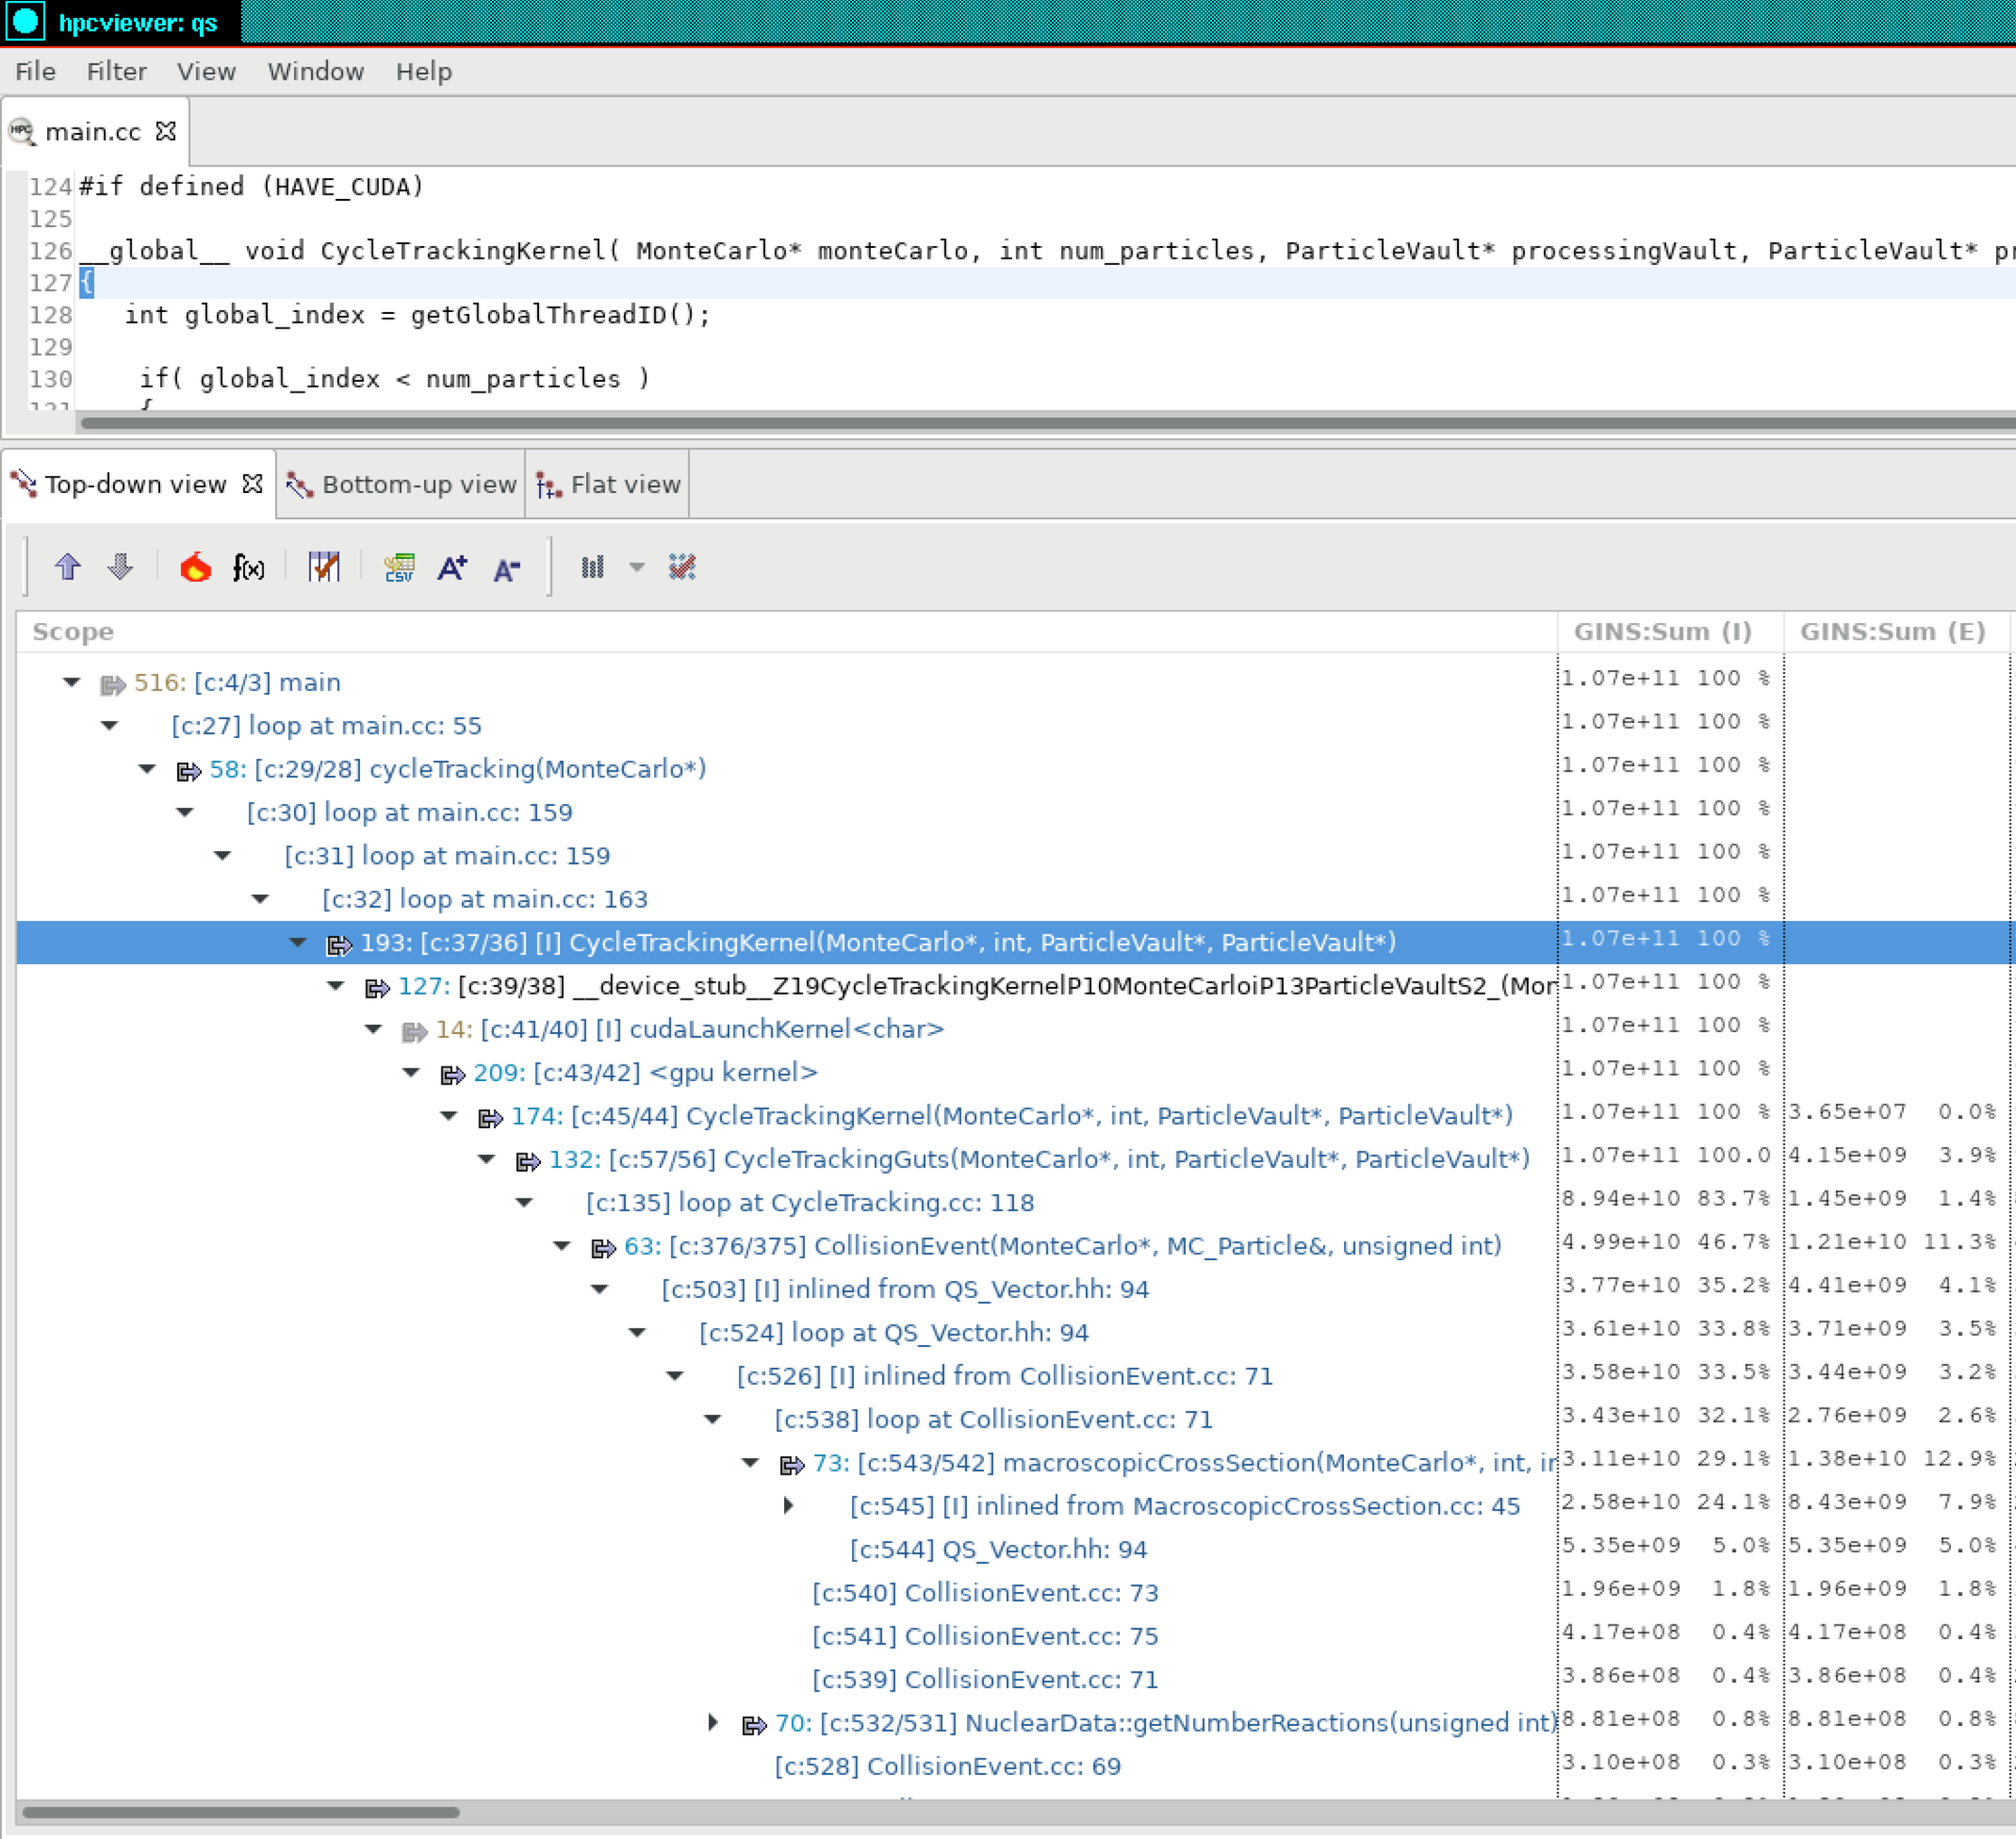
\includegraphics[width=\textwidth]{qs-cct.pdf}
\caption{A screenshot of \hpcviewer{} for the GPU-accelerated Quicksilver proxy app with GPU CCT reconstruction.}
\label{qs-cct}
\end{figure}

Figure~\ref{fig:gpu calling context tree} illustrates the reconstruction of an approximate calling context tree for a GPU computation given the static call graph (computed by \hpcstruct{} from a CUBIN's machine instructions) and PC sample counts for some or all GPU instructions in the CUBIN. Figure~\ref{qs-cct} shows an \hpcviewer{} screenshot for the GPU-accelerated Quicksilver proxy app following reconstruction of GPU calling contexts using the algorithm described in this section. Notice that after the reconstruction, one can see that \verb|CycleTrackingKernel| calls \verb|CycleTrackingGuts|, which calls \verb|CollisionEvent|, which eventually calls  \verb|macroscopicCrossSection| and \verb|NuclearData::getNumberOfReactions|. The the rich  approximate GPU calling context tree reconstructed by \hpcprof{} also shows loop nests and inlined code.\footnote{The control flow graph used to produce this reconstruction for Quicksilver was computed with a pre-release version of {\tt nvdisasm}. You will not be able to reproduce these results with CUDA 10's {\tt nvdisasm} because the released version of {\tt nvdisasm} fails to analyze some of the key functions in Quicksilver.}



\section{AMD GPUs}

HPCToolkit provides {\em alpha}-level support for coarse-grain profiling of GPU-accelerated  applications that offload computation onto AMD GPUs using  AMD's HIP programming model. Table~\ref{amd-options} shows arguments to \hpcrun{} to monitor the performance of GPU operations on AMD GPUs. With this coarse-grain profiling support, HPCToolkit can collect GPU operation timings (Table~\ref
{table:gtimes}) and a subset of standard metrics for GPU operations such as memory allocation and deallocation (Table~\ref{table:gmem}), memory set (Table~\ref{table:gmset}), explicit memory copies (Table~\ref{table:gxcopy}), and synchronization (Table~\ref{table:gsync}). 

\begin{table}[t]
\centering
\begin{tabular}{|l|p{3.5in}|}\hline
Argument to \hpcrun{} & What is monitored\\\hline\hline
{\tt -e gpu=amd} & profiling of AMD GPU operations\\\hline
{\tt -e gpu=amd -t} & profiling and tracing of AMD GPU operations\\\hline
\end{tabular}
\caption{Monitoring performance on AMD GPUs.}
\label{amd-options}
\end{table}

At present, HPCToolkit's support for monitoring on AMD GPUs is incomplete. The HPCToolkit team is awaiting enhancements to AMD's ROC-tracer monitoring library that are needed to complete support for adding GPU kernels to call paths collected at the point where GPU operations are invoked. Currently, the leaves of call paths  for GPU kernel invocations end in the placeholder \verb|<gpu kernel>| and lack the name of the kernel invoked. This more greatly affects trace lines for GPU streams in \hpctraceviewer{} where one can only see GPU activity marked by \verb|<gpu kernel>| without being able to readily identify the specific kernels being invoked. The HPCToolkit project team is awaiting completion of additional support in AMD's ROC-tracer monitoring library to address this deficiency.

At present, ROC-tracer lacks support for fine-grain performance measurement of GPU computations on AMD GPUs like the PC sampling supported by NVIDIA's GPUs.

\section{Intel GPUs}

HPCToolkit does not yet support measurement and analysis of performance on Intel GPUs.





% ***************************************************************************
% ***************************************************************************

\chapter{Measurement and Analysis of OpenMP Multithreading}
\label{chpt:gpu}

{
\centering
 \fbox{\parbox{\textwidth}{Note: This release contains beta support for monitoring OpenMP computations using the OpenMP 5.0 OpenMP Tools API support known as OMPT.}}
 \vspace{2ex}
}

HPCToolkit includes an implementation of the OpenMP 5.0 Tools API known as OMPT. The OMPT interface enables HPCToolkit to extract enough information to reconstruct user-level calling contexts from implementation-level measurements. 

Support for OpenMP 5.0 and OMPT is emerging in OpenMP runtimes. Recent versions of LLVM's OpenMP runtime, IBM's LOMP (Lightweight OpenMP Runtime) and Intel's OpenMP runtime provide emerging support for OMPT. At present, support in these implementations is known to be incomplete, especially with respect to offloading computation onto TARGET devices. 

If an interaction between HPCToolkit's support for the OMPT interface and an OpenMP runtime causes problems, OMPT support may be disabled when using HPCToolkit by setting  OpenMP environment variable {\tt OMP\_TOOL} to {\tt disabled}.




% ***************************************************************************
% ***************************************************************************

\chapter{The \hpcviewer{} User Interface}
\label{chpt:hpcviewer-interface}

%% $Id$

%%%%%%%%%%%%%%%%%%%%%%%%%%%%%%%%%%%%%%%%%%%%%%%%%%%%%%%%%%%%%%%%%%%%%%%%%%%%%
%%%%%%%%%%%%%%%%%%%%%%%%%%%%%%%%%%%%%%%%%%%%%%%%%%%%%%%%%%%%%%%%%%%%%%%%%%%%%

\documentclass[english]{article}
\usepackage[latin1]{inputenc}
\usepackage{babel}
\usepackage{verbatim}

%% do we have the `hyperref package?
\IfFileExists{hyperref.sty}{
   \usepackage[bookmarksopen,bookmarksnumbered]{hyperref}
}{}

%% do we have the `fancyhdr' or `fancyheadings' package?
\IfFileExists{fancyhdr.sty}{
\usepackage[fancyhdr]{latex2man}
}{
\IfFileExists{fancyheadings.sty}{
\usepackage[fancy]{latex2man}
}{
\usepackage[nofancy]{latex2man}
\message{no fancyhdr or fancyheadings package present, discard it}
}}

%% do we have the `rcsinfo' package?
\IfFileExists{rcsinfo.sty}{
\usepackage[nofancy]{rcsinfo}
\rcsInfo $Id$
\setDate{\rcsInfoLongDate}
}{
\setDate{ 2012/09/21}
\message{package rcsinfo not present, discard it}
}

\setVersionWord{Version:}  %%% that's the default, no need to set it.
\setVersion{=PACKAGE_VERSION=}

%%%%%%%%%%%%%%%%%%%%%%%%%%%%%%%%%%%%%%%%%%%%%%%%%%%%%%%%%%%%%%%%%%%%%%%%%%%%%
%%%%%%%%%%%%%%%%%%%%%%%%%%%%%%%%%%%%%%%%%%%%%%%%%%%%%%%%%%%%%%%%%%%%%%%%%%%%%

\begin{document}

\begin{Name}{1}{hpcviewer}{The HPCToolkit Performance Tools}{The HPCToolkit Performance Tools}{hpcviewer:\\ Interactive Presentation of Performance}

The Java-based \Prog{hpcviewer} interactively presents program performance in a top-down fashion.

\end{Name}

%%%%%%%%%%%%%%%%%%%%%%%%%%%%%%%%%%%%%%%%%%%%%%%%%%%%%%%%%%%%%%%%%%
\section{Synopsis}

Command-line usage:\\
\SP\SP\SP\Prog{hpcviewer} \oOpt{options} \oOpt{hpctoolkit-database}

GUI usage:\\
\SP\SP\SP Launch \File{hpcviewer} and open the Experiment database \oOpt{hpctoolkit-database}.


%%%%%%%%%%%%%%%%%%%%%%%%%%%%%%%%%%%%%%%%%%%%%%%%%%%%%%%%%%%%%%%%%%
\section{Description}

The Java-based \Prog{hpcviewer} interactively presents program-performance Experiment databases in a top-down fashion.
Since Experiment databases are self-contained, they may be relocated from a cluster for visualization on a laptop or workstation.

%%%%%%%%%%%%%%%%%%%%%%%%%%%%%%%%%%%%%%%%%%%%%%%%%%%%%%%%%%%%%%%%%%
\section{Arguments}

\begin{Description}
\item[\Arg{hpctoolkit-database}] An HPCToolkit Experiment database, which is the result of executing \Prog{hpcprof}, \Prog{hpcprof-mpi} or \Prog{hpcprof-flat}.
\end{Description}

%Default values for an option's optional arguments are shown in \{\}.

\subsection{Options}

\begin{Description}
\item[\Opt{-n}]
Do not display the Callers View.  (Saves memory and time.)

\item[\Opt{-consolelog}]
Send log entries to a console in addition to a log file.

\item[\Opt{-debug}]
Log additional information about plug-in dependency problems.

\end{Description}


%%%%%%%%%%%%%%%%%%%%%%%%%%%%%%%%%%%%%%%%%%%%%%%%%%%%%%%%%%%%%%%%%%
\section{Detailed Description}

\subsection{Views}

\Prog{hpcviewer} supports three principal views of an application's performance data.  Both inclusive (costs of a procedure including all its callees) and exclusive costs (costs excluding callees) are reported.

\begin{itemize}
  \item \textbf{Calling context view.}
A top-down view that represents the dynamic calling contexts (call paths) in which costs were incurred.
Using this view, one can explore performance measurements of an application in a top-down fashion to understand the costs incurred by calls to a procedure in a particular calling context.

  \item \textbf{Callers view.}
This bottom-up view enables one to look upward along call paths.
The view apportions a procedure's costs to its caller and, more generally, its calling contexts.
This view is particularly useful for understanding the performance of software components or procedures that are used in more than one context.

  \item \textbf{Flat view.}
This view organizes performance measurement data according to the static structure of an application.
All costs incurred in \emph{any} calling context by a procedure are aggregated together in the flat view.
\end{itemize}


\subsection{Panes}

The browser window is divided into three panes:

\begin{itemize}
  \item \textbf{Source pane.} The source code associated with the current entity selected in the navigation pane.
Selecting any entity in the navigation pane will cause the source pane to load the corresponding file, scroll to and highlight the line corresponding to the selection.

\item \textbf{Navigation pane.}
The navigation pane presents a hierarchical tree-based structure that is used to organize the presentation of an application's performance data.
Entities that occur in the navigation pane's tree include load modules, files, procedures, procedure activations, inlined code, loops, and source lines.
Entities can be selected; and children can be revealed or concealed.

The nature of the entities in the navigation pane's tree structure depends upon whether one is exploring the calling context view, the callers view, or the flat view of the performance data. 

\begin{itemize}
\item In the calling context view, entities in the navigation tree represent procedure activations, inlined code, loops, and source lines. 
While most entities link to a single location in source code, procedure activations link to two: the call site from which a procedure was called and the procedure itself.
\item In the callers view, entities in the navigation tree are procedure activations. Unlike procedure activations in the calling context tree view in which call sites are paired with the called procedure, in the caller's view, call sites are paired with the calling procedure to facilitate attribution of costs for a called procedure to multiple different call sites and callers.
\item In the flat view, entities in the navigation tree correspond to source files, procedure call sites (which are rendered the same way as procedure activations), loops, and source lines.
\end{itemize}


The header above the navigation pane contains flatten and zoom control.
\begin{itemize}
\item \textbf{Up arrow.} Zooms to show only information for the selected line and its descendants.
\item \textbf{Down arrow.} Zooms out (reversing a prior zoom operation).
\item \textbf{Hot path}. The button activates "\emph{hot path analysis}", which automatically expands the scopes along the hot path for the selected metric in the subtree rooted at the selected scope. It is a convenient way to find a performance bottleneck of a given metric.
\item \textbf{Derived metric}. Creation of a new metric based on spreadsheet-like mathematical formulae.
\item \textbf{Filter metrics}. Show or hide metrics.
\item \textbf{CSV export}. Export information from the current view to a comma separated values (CSV) file.
\item \textbf{Bigger font}. Change the current font with a bigger size font.
\item \textbf{Smaller font}. Change the current font with a smaller size font.
\item \textbf{Flatten.} (flat view only) Flattening (the icon that shows a tree node with a slash through it) replaces each top-level scope shown with its children. If a scope has no children (i.e., it is a leaf), the node will remain in the view. This flattening operation is useful for relaxing the strict hierarchical view so that peers at the same level in the tree can be viewed and ranked together. For instance, this can be used to hide procedures in the flat view so that outermost loops can be ranked and compared to one another.
\item \textbf{Unflatten.} (flat view only) The inverse of the flatten operation, making an elided node visible again.

\end{itemize}

\item  \textbf{Metric pane.}
The metric pane displays one or more performance metrics associated with entities to the left in the navigation pane.
Entities in the tree view of the navigation pane are sorted at each level of the hierarchy by the metric in the selected column.

\end{itemize}


\subsection{Thread-Centric Plots}

\Prog{hpcviewer} can display plot graphs of thread-level metric
values.  This is useful for quickly assessing load imbalance across
processes and threads.

To create a graph, use the calling context view and select a scope by
left-clicking a line in the navigation pane.
Then, right-click the selected scope to show the context menu.  (This
menu begins with `Zoom-in' and `Zoom-out.')
At the bottom of the context menu is a list of metrics that
\Prog{hpcviewer} can graph.
Each metric contains a sub-menu that lists the three different types
of graphs that \Prog{hpcviewer} can plot.
The \emph{Plot} graph sorts the processes by process and thread
number.
The \emph{Sorted plot} graph sorts the processes by metric value.
And the \emph{Histogram} graph shows a bar graph of the
frequency of metric values.

Note: currently, these plot graphs are available only with databases
created by \Prog{hpcprof-mpi} and not by \Prog{hpcprof}.
See the section on ``\emph{Plotting Graphs of Thread-level Metric Values}''
in the User's Manual for more description and a view of a plot graph.


%%%%%%%%%%%%%%%%%%%%%%%%%%%%%%%%%%%%%%%%%%%%%%%%%%%%%%%%%%%%%%%%%%
%\section{Arguments}

%%%%%%%%%%%%%%%%%%%%%%%%%%%%%%%%%%%%%%%%%%%%%%%%%%%%%%%%%%%%%%%%%%
%\section{Examples}

%%%%%%%%%%%%%%%%%%%%%%%%%%%%%%%%%%%%%%%%%%%%%%%%%%%%%%%%%%%%%%%%%%
%\section{Notes}

%%%%%%%%%%%%%%%%%%%%%%%%%%%%%%%%%%%%%%%%%%%%%%%%%%%%%%%%%%%%%%%%%%
\section{See Also}

\HTMLhref{hpctoolkit.html}{\Cmd{hpctoolkit}{1}}.

%%%%%%%%%%%%%%%%%%%%%%%%%%%%%%%%%%%%%%%%%%%%%%%%%%%%%%%%%%%%%%%%%%
\section{Version}

Version: \Version\ of \Date.

%%%%%%%%%%%%%%%%%%%%%%%%%%%%%%%%%%%%%%%%%%%%%%%%%%%%%%%%%%%%%%%%%%
\section{License and Copyright}

\begin{description}
\item[Copyright] \copyright\ 2002-2014, Rice University.
\item[License] See \File{README.License}.
\end{description}

%%%%%%%%%%%%%%%%%%%%%%%%%%%%%%%%%%%%%%%%%%%%%%%%%%%%%%%%%%%%%%%%%%
\section{Authors}

\noindent
Laksono Adhianto \\
John Mellor-Crummey \\
Nathan Tallent \\
Rice HPCToolkit Research Group \\
Email: \Email{hpctoolkit-forum =at= rice.edu} \\
WWW: \URL{http://hpctoolkit.org}.

\LatexManEnd

\end{document}

%% Local Variables:
%% eval: (add-hook 'write-file-hooks 'time-stamp)
%% time-stamp-start: "setDate{ "
%% time-stamp-format: "%:y/%02m/%02d"
%% time-stamp-end: "}\n"
%% time-stamp-line-limit: 50
%% End:




% ***************************************************************************
% ***************************************************************************

\chapter{The \hpctraceviewer{} User Interface}
\label{chpt:hpctraceviewer-interface}

%% $Id: hpctraceviewer.tex 3428 2011-02-22 21:31:42Z tallent $

%%%%%%%%%%%%%%%%%%%%%%%%%%%%%%%%%%%%%%%%%%%%%%%%%%%%%%%%%%%%%%%%%%%%%%%%%%%%%
%%%%%%%%%%%%%%%%%%%%%%%%%%%%%%%%%%%%%%%%%%%%%%%%%%%%%%%%%%%%%%%%%%%%%%%%%%%%%

\documentclass[english]{article}
\usepackage[latin1]{inputenc}
\usepackage{babel}
\usepackage{verbatim}

%% do we have the `hyperref package?
\IfFileExists{hyperref.sty}{
   \usepackage[bookmarksopen,bookmarksnumbered]{hyperref}
}{}

%% do we have the `fancyhdr' or `fancyheadings' package?
\IfFileExists{fancyhdr.sty}{
\usepackage[fancyhdr]{latex2man}
}{
\IfFileExists{fancyheadings.sty}{
\usepackage[fancy]{latex2man}
}{
\usepackage[nofancy]{latex2man}
\message{no fancyhdr or fancyheadings package present, discard it}
}}

\setDate{2020/06/02}

\setVersionWord{Version:}  %%% that's the default, no need to set it.
\setVersion{=PACKAGE_VERSION=}

%%%%%%%%%%%%%%%%%%%%%%%%%%%%%%%%%%%%%%%%%%%%%%%%%%%%%%%%%%%%%%%%%%%%%%%%%%%%%
%%%%%%%%%%%%%%%%%%%%%%%%%%%%%%%%%%%%%%%%%%%%%%%%%%%%%%%%%%%%%%%%%%%%%%%%%%%%%

\begin{document}



\begin{Name}{1}{hpctraceviewer}{The HPCToolkit Performance Tools}{The HPCToolkit Performance Tools}{hpctraceviewer:\\ Interactive Presentation of Program Traces}

The Java-based \Prog{hpctraceviewer} interactively presents dynamic behavior of a program. 

\end{Name}

%%%%%%%%%%%%%%%%%%%%%%%%%%%%%%%%%%%%%%%%%%%%%%%%%%%%%%%%%%%%%%%%%%
\section{Synopsis}

Command-line usage:\\
\SP\SP\SP\Prog{hpctraceviewer} \oOpt{options} \oOpt{hpctoolkit-database}

GUI usage:\\
\SP\SP\SP Launch \File{hpctraceviewer} and open the Experiment database \oOpt{hpctoolkit-database}.


%%%%%%%%%%%%%%%%%%%%%%%%%%%%%%%%%%%%%%%%%%%%%%%%%%%%%%%%%%%%%%%%%%
\section{Description}

The Java-based \Prog{hpctraceviewer} interactively presents program traces in a top-down fashion.
Since Experiment databases are self-contained, they may be relocated from a cluster for visulization on a laptop or workstation.

%%%%%%%%%%%%%%%%%%%%%%%%%%%%%%%%%%%%%%%%%%%%%%%%%%%%%%%%%%%%%%%%%%
\section{Arguments}

\begin{Description}
\item[\Arg{hpctoolkit-database}] An HPCToolkit Experiment database, which is the result of executing \Prog{hpcprof}, \Prog{hpcprof-mpi} or \Prog{hpcprof-flat}.
\end{Description}

%Default values for an option's optional arguments are shown in \{\}.

\subsection{Options}

\begin{Description}

\item[\Opt{-consolelog}]
Send log entries to a console in addition to a log file.

\item[\Opt{-debug}]
Log additional information about plug-in dependency problems.

\end{Description}


%%%%%%%%%%%%%%%%%%%%%%%%%%%%%%%%%%%%%%%%%%%%%%%%%%%%%%%%%%%%%%%%%%
\section{Detailed Description}

\subsection{Views}

\Prog{hpctraceviewer} comprises of three different parts. 


\begin{itemize}
\item \textbf{Trace view} (top, left pane):
  This is hpctraceviewer's primary view.
  This view, which is similar to a conventional process/time (or space/time) view, shows time on the horizontal axis and process (or thread) rank on the vertical axis; time moves from left to right.
  Compared to typical process/time views, there is one key difference.
  To show call path hierarchy, the view is actually a user-controllable slice of the process/time/call-path space.
  Given a call path depth, the view shows the color of the currently active procedure at a given time and process rank.
  (If the requested depth is deeper than a particular call path, then hpctraceviewer simply displays the deepest procedure frame and, space permitting, overlays an annotation indicating the fact that this frame represents a shallower depth.)
  hpctraceviewer assigns colors to procedures based on (static) source code procedures.
  Although the color assignment is currently random, it is consistent across the different views.
  Thus, the same color within the Trace and Depth Views refers to the same procedure.
  The Trace View has a white crosshair that represents a selected point in time and process space.
  For this selected point, the Call Path View shows the corresponding call path.
  The Depth View shows the selected process.

\item \textbf{Depth view} (tab in bottom, left pane):
  This is a call-path/time view for the process rank selected by the Trace view's crosshair.
  Given a process rank, the view shows for each virtual time along the horizontal axis a stylized call path along the vertical axis, where `main' is at the top and leaves (samples) are at the bottom.
  In other words, this view shows for the whole time range, in qualitative fashion, what the Call Path View shows for a selected point.
  The horizontal time axis is exactly aligned with the Trace View's time axis; and the colors are consistent across both views.
  This view has its own crosshair that corresponds to the currently selected time and call path depth.

\item \textbf{Summary view} (tab in bottom, left pane):
  The view shows for the whole time range dislayed, the proportion of each subroutine in a certain time.
  Similar to Depth view, the time range in Summary reflects to the time range in the Trace view. 

\item \textbf{Call Path view} (tab in top, right pane):
  This view shows two things: (1) the current call path depth that defines the hierarchical slice shown in the Trace View; and (2) the actual call path for the point selected by the Trace View's crosshair.
  (To easily coordinate the call path depth value with the call path, the Call Path View currently suppresses details such as loop structure and call sites; we may use indentation or other techniques to display this in the future.)

\item \textbf{Statistics view} (tab in top, right pane)
  The view shows a list of procedures and the estimated execution percentage for each for the time interval currently shown in the Trace view. 
  Whenever the user changes the time interval displayed in the Trace view, the statistics view will update its list of procedures and their execution percentages to 
  reflect the current interval.  Similarly, a change in the selected call path depth will also update the contents of the statistics view.

\item \textbf{Mini map view} (bottom, right pane):
  The Mini Map shows, relative to the process/time dimensions, the region of the execution shown by the Trace View.
  In the Mini map, dragging the selected region or making a new selection enables one to change the region of the trace that is the current focus for analysis.

\end{itemize}


% ===========================================================================

\subsection{Trace view}

Trace view is divided into two parts: the top part which contains \emph{action pane} and the \emph{information pane}, and the main view which displays the traces. 

The buttons in the action pane are the following:
\begin{itemize}

\item Home : Resetting the view configuration into the original view, i.e., viewing traces for all times and processes.
\item Horiontal zoom in / out : Zooming in/out the time dimension of the traces. 
\item Vertical zoom in / out : Zooming in/out the process dimension of the traces.
\item Navigation buttons : Navigating the trace view to the left, right, up and bottom, respectively. It is also possible to navigate with the arrow keys in the keyboard. Since Trace view does not support scrool bars, the only way to navigate is through navigation buttons (or arrow keys).
\item Undo : Canceling the action of zoom or navigation and returning back to the previous view configuration.
\item Redo : Redoing of previously undo change of view configuration.
\item save  / a view configuration : Saving/loading a saved view configuration. 
A view configuration file contains the information of the current dimension of time and process, the depth and the position of the crosshair. 
It is recommended to store the view configuration file in the same directory as the database to ensure that the view configuration file matches well with the database since the file does not store which database it is associated with. 
Although it is possible to open a view configuration file which is associated from different database, it is highly not recommended since each database has different time/process dimensions and depth.


\end{itemize}

The information pane contains some information concerning the range status of the current displayed data.
\begin{itemize}
 \item Time Range. The information of current time-range (horizontal) dimension. 
 \item Process Range. The information of current process-range (vertical) dimension. 
 \item Cross Hair. The information of current crosshair position in time and process dimensions. 
\end{itemize}


% ===========================================================================
% ===========================================================================
\subsection{Depth view}

Depthview shows all the call path for a certain time range [t_1,t_2]= \{t | t_1 <= t <= t_2\} in a specified process rank $p$. The content of Depth view is always consistent with the position of the cross-hair in Trace view.
For instance once the user clicks in process $p$ and time $t$, while the current depth of call path is $d$, then the Depth view's content is updated to display all the call path of process $p$ and shows its cross-hair on the time $t$ and the call path depth $d$.

On the other hand, any user action such as cross-hair and time range selection in Depth view will update the content within Trace view. Similarly, the selection of new call path depth in Call view invokes a new position in Depth view.

In Depth view a user can specify a new cross-hair time and a new time range.

\textbf{Specifying a new cross-hair time.} Selecting a new cross-hair time $t$ can be performed by clicking a pixel within Depth view. This will update the cross-hair in Trace view and the call path in Call view.

\textbf{Selecting a new time range.} Selecting a new time range [t_m,t_n]= \{t | t_m <= t <= t_n\} is performed by first clicking the position of $t_m$ and drag the cursor to the position of $t_n$. A new content in Depth view and Trace view is then updated. Note that this action will not update the call path in Call view since it does not change the position of the cross-hair.


% ===========================================================================
% ===========================================================================
\subsection{Summary view}

Summary view presents the proportion of number of calls of time $t$ across the current displayed rank of proces $p$. 
Similar to Depth view, the time range in Summary view is always consistent with the time range in Trace view.


% ===========================================================================
% ===========================================================================
\subsection{Call view}

This view lists the call path of process \textbf{p} and time \textbf{t} specified in Trace view and Depth view.
This view can show a call path from depth $0$ to the maximum depth, and the current depth is shown in the depth editor (located on the top part of the view).

In this view, the user can select the depth dimension by either typing the depth in the depth editor or selecting a procedure in the table of call path.

% ===========================================================================
% ===========================================================================
\subsection{Mini view}

The Mini view shows, relative to the process/time dimensions, the portion of the execution shown by the Trace view.
In Mini view, the user can select a new process/time (p_a,t_a),(p_b,t_b) dimensions by clicking the first process/time position (p_a,t_a) and then drag the cursor to the second position (p_b,t_b).
The user can also moving the current selected region to another region by clicking the white rectangle and drag it to the new place.



% ===========================================================================
% ===========================================================================

\section{Menus}
\Prog{hpctraceviewer} provides three main menus:
\begin{itemize}
 \item \textbf{File} menu which contains two sub menus:
 \begin{itemize}
   \item \textbf{Open database}: to load a database experiment directory. The directory has to contain \texttt{experiment.xml} (CCT and metric information) or \texttt{callpath.xml} (uniquely CCT information), and \texttt{*.hpctrace} or \texttt{experiment.mt} files which provide trace information.
   \item \textbf{Exit}: to quit the application.
 \end{itemize}
 \item \textbf{View} menu to enhance appearance which contains two sub menus:
 \begin{itemize}
   \item \textbf{Show debug info}: to enable/disabe the display of debugging information in the form of \textbf{`a(b)'} where \textbf{a} is the maximum depth (this number is shown if the current depth reaches the maximum depth) and \textbf{b} is the number of records on the trace view. 
The number of records can be useful to identify blocking procedures (such as I/O operations). Note: the numbers are displayed only if there's enough space in the process time line.
   \item \textbf{Using midpoint painting}: if checked, the trace painting will use {midpoint} painting algorithm. By using the later, for every samples $S1$ at time $T1$, $S2$ at time $T2$ and $S3$ at time $T3$, \Prog{hpctraceviewer} renders a block from $T1$ to $(T1+T2)/2$ to sample $S1$, and a block from from  $(T1+T2)/2$ to  $(T2+T3(/2$ for sample $S2$, and so forth. 
If the menu is not checked, then a simpler {rightmost} algorithm is used: it will render a block from  $T1$ to $T2$ for sample $S1$, and a block from $T2$ to  $T3$ for sample $S2$, and so forth.
   \item \textbf{Show procedure-color mapping}: to open a window which shows customized mapping between a procedure pattern and a color. \Prog{hpctraceviewer} allows users to customize assignment of a pattern of procedure names with a specific color.
   \item \textbf{Filter ranks}: to open a window for selecting which ranks and/or threads should be displayed or hidden. 
Recall that a rank can be a process (e.g. MPI applications), a thread (OpenMP applications) or a process/thread pair (hybrid MPI and OpenMP applications). 
\Prog{hpctraceviewer} allows two types of filtering: either you specify which ranks {to show} or {to hide} (default is to hide). 
To add a pattern to filter, you need to click the "Add" button and type the pattern in the format \texttt{minimum:maximum:stride}. \\
For instance, \texttt{3:7:2} in the process box with the thread box empty will match all threads of processes 3, 5, and 7.\\
To remove a pattern, you have to select the pattern to remove, and click the "Remove" button. Finally, clicking to "Remove all" button will clear the list of patterns.
 \end{itemize}
 \item \textbf{Window} menu to manage the layout of the application. The menu only provide one sub menu:
 \begin{itemize}
  \item \textbf{Reset layout}: to reset the layout to the original one.
 \end{itemize}
\end{itemize}

\Prog{hpctraceviewer} also provides a context menu to save the current image of the view. 
This context menu is available is three views: trace view, depth view and summary view.
% ===========================================================================



%%%%%%%%%%%%%%%%%%%%%%%%%%%%%%%%%%%%%%%%%%%%%%%%%%%%%%%%%%%%%%%%%%
%\section{Arguments}

%%%%%%%%%%%%%%%%%%%%%%%%%%%%%%%%%%%%%%%%%%%%%%%%%%%%%%%%%%%%%%%%%%
%\section{Examples}

%%%%%%%%%%%%%%%%%%%%%%%%%%%%%%%%%%%%%%%%%%%%%%%%%%%%%%%%%%%%%%%%%%
%\section{Notes}

%%%%%%%%%%%%%%%%%%%%%%%%%%%%%%%%%%%%%%%%%%%%%%%%%%%%%%%%%%%%%%%%%%
\section{See Also}

\HTMLhref{hpctoolkit.html}{\Cmd{hpctoolkit}{1}}.

%%%%%%%%%%%%%%%%%%%%%%%%%%%%%%%%%%%%%%%%%%%%%%%%%%%%%%%%%%%%%%%%%%
\section{Version}

Version: \Version

%%%%%%%%%%%%%%%%%%%%%%%%%%%%%%%%%%%%%%%%%%%%%%%%%%%%%%%%%%%%%%%%%%
\section{License and Copyright}

\begin{description}
\item[Copyright] \copyright\ 2002-2020, Rice University.
\item[License] See \File{README.License}.
\end{description}

%%%%%%%%%%%%%%%%%%%%%%%%%%%%%%%%%%%%%%%%%%%%%%%%%%%%%%%%%%%%%%%%%%
\section{Authors}

\noindent
Rice University's HPCToolkit Research Group \\
Email: \Email{hpctoolkit-forum =at= rice.edu} \\
WWW: \URL{http://hpctoolkit.org}.

\LatexManEnd

\end{document}

%% Local Variables:
%% eval: (add-hook 'write-file-hooks 'time-stamp)
%% time-stamp-start: "setDate{ "
%% time-stamp-format: "%:y/%02m/%02d"
%% time-stamp-end: "}\n"
%% time-stamp-line-limit: 50
%% End:




% ***************************************************************************
% ***************************************************************************

\chapter{Monitoring MPI Applications}
\label{chpt:mpi-apps}

\HPCToolkit{}'s measurement subsystem can measure each process and thread in an execution of an MPI program.
\HPCToolkit{} can be used with pure MPI programs as well as hybrid programs that use multithreading, e.g. OpenMP or Pthreads, within MPI processes.

\HPCToolkit{} supports C, C++ and Fortran MPI programs.
It has been successfully tested with MPICH, MVAPICH and OpenMPI and should work with almost all MPI implementations.


% ===========================================================================
% ===========================================================================

\section{Running and Analyzing MPI Programs}

\newcommand{\question}[1]{\vspace{4pt}\par\noindent{\bf Q: #1}}
\newcommand{\answer}{\par\vspace{2pt}\noindent{\bf A:}}

\question{How do I launch an MPI program with hpcrun?}

\answer{}
For a dynamically linked application binary \texttt{app}, use a command line similar to the following example:
%
\begin{quote}
  \verb|<mpi-launcher> hpcrun -e <event>:<period> ... app [app-arguments]|
\end{quote}
%
Observe that the MPI launcher (\texttt{mpirun}, \texttt{mpiexec}, \etc{}) is used to launch \hpcrun{}, which is then used to launch the application program.

\vspace{1ex}

\question{How do I compile and run a statically linked MPI program?}

\answer{}
On systems such IBM's Blue Gene/Q microkernel that are designed to run statically linked binaries, use \hpclink{} to build a statically linked version of your application that includes \HPCToolkit{}'s monitoring library.
For example, to link your application binary \texttt{app}:
%
\begin{quote}
\begin{verbatim}
hpclink <linker> -o app <linker-arguments>
\end{verbatim}
\end{quote}
%
Then, set the \mytt{HPCRUN_EVENT_LIST} environment variable in the launch script before running the application:
%
\begin{quote}
\begin{verbatim}
export HPCRUN_EVENT_LIST="CYCLES@f200"
<mpi-launcher> app [app-arguments]
\end{verbatim}
%
\end{quote}
See the Chapter~\ref{chpt:statically-linked-apps} for more information.

\vspace{1ex}

\question{What files does \hpcrun{} produce for an MPI program?}

\answer{}
In this example, \mytt{s3d_f90.x} is the Fortran S3D program compiled with OpenMPI and run with the command line
%
\begin{quote}
  \verb|mpiexec -n 4 hpcrun -e PAPI_TOT_CYC:2500000 ./s3d_f90.x|
\end{quote}
%
This produced 12 files in the following abbreviated \texttt{ls} listing:
%
\begin{quote}
\begin{verbatim}
krentel 1889240 Feb 18  s3d_f90.x-000000-000-72815673-21063.hpcrun
krentel    9848 Feb 18  s3d_f90.x-000000-001-72815673-21063.hpcrun
krentel 1914680 Feb 18  s3d_f90.x-000001-000-72815673-21064.hpcrun
krentel    9848 Feb 18  s3d_f90.x-000001-001-72815673-21064.hpcrun
krentel 1908030 Feb 18  s3d_f90.x-000002-000-72815673-21065.hpcrun
krentel    7974 Feb 18  s3d_f90.x-000002-001-72815673-21065.hpcrun
krentel 1912220 Feb 18  s3d_f90.x-000003-000-72815673-21066.hpcrun
krentel    9848 Feb 18  s3d_f90.x-000003-001-72815673-21066.hpcrun
krentel  147635 Feb 18  s3d_f90.x-72815673-21063.log
krentel  142777 Feb 18  s3d_f90.x-72815673-21064.log
krentel  161266 Feb 18  s3d_f90.x-72815673-21065.log
krentel  143335 Feb 18  s3d_f90.x-72815673-21066.log
\end{verbatim}
\end{quote}
%
Here, there are four processes and two threads per process.
Looking at the file names, \mytt{s3d_f90.x} is the name of the program binary, \mytt{000000-000} through \mytt{000003-001} are the MPI rank and thread numbers, and \mytt{21063} through \mytt{21066} are the process IDs.

We see from the file sizes that OpenMPI is spawning one helper thread per process.
Technically, the smaller \mytt{.hpcrun} files imply only a smaller calling-context tree (CCT), not necessarily fewer samples.
But in this case, the helper threads are not doing much work.


\vspace{1ex}

\question{Do I need to include anything special in the source code?}

\answer{}
Just one thing.
Early in the program, preferably right after \mytt{MPI_Init()}, the program should call \mytt{MPI_Comm_rank()} with communicator \mytt{MPI_COMM_WORLD}.
Nearly all MPI programs already do this, so this is rarely a problem.
For example, in C, the program might begin with:
%
\begin{quote}
\begin{verbatim}
int main(int argc, char **argv)
{
    int size, rank;

    MPI_Init(&argc, &argv);
    MPI_Comm_size(MPI_COMM_WORLD, &size);
    MPI_Comm_rank(MPI_COMM_WORLD, &rank);
    ...
}
\end{verbatim}
\end{quote}

\emph{Note:} The first call to \mytt{MPI_Comm_rank()} should use \mytt{MPI_COMM_WORLD}.
This sets the process's MPI rank in the eyes of \hpcrun{}.
Other communicators are allowed, but the first call should use \mytt{MPI_COMM_WORLD}.

Also, the call to \mytt{MPI_Comm_rank()} should be unconditional, that is all processes should make this call.
Actually, the call to \mytt{MPI_Comm_size()} is not necessary (for \hpcrun{}), although most MPI programs normally call both \mytt{MPI_Comm_size()} and \mytt{MPI_Comm_rank()}.

\vspace{1ex}

\question{What MPI implementations are supported?}

\answer{}
Although the matrix of all possible MPI variants, versions, compilers, architectures and systems is very large, \HPCToolkit{} has been tested successfully with MPICH, MVAPICH and OpenMPI and should work with most MPI implementations.

\vspace{1ex}

\question{What languages are supported?}

\answer{}
C, C++ and Fortran are supported.

% ===========================================================================
% ===========================================================================

\section{Building and Installing \HPCToolkit{}}

\question{Do I need to compile \HPCToolkit{} with any special options for MPI support?}

\answer{}
No, \HPCToolkit{} is designed to work with multiple MPI implementations at the same time.
That is, you don't need to provide an \mytt{mpi.h} include path, and you don't need to compile multiple versions of \HPCToolkit{}, one for each MPI implementation.

The technically-minded reader will note that each MPI implementation uses a different value for \mytt{MPI_COMM_WORLD} and may wonder how this is possible.
\hpcrun{} (actually \mytt{libmonitor}) waits for the application to call \mytt{MPI_Comm_rank()} and uses the same communicator value that the application uses.
This is why we need the application to call \mytt{MPI_Comm_rank()} with communicator \mytt{MPI_COMM_WORLD}.


% ***************************************************************************
% ***************************************************************************

\chapter{Monitoring Statically Linked Applications}
\label{chpt:statically-linked-apps}


% ===========================================================================
% ===========================================================================

On modern Linux systems, dynamically linked executables are the default.
With dynamically linked executables, \HPCToolkit{}'s \hpcrun{} script uses library preloading to inject \HPCToolkit's monitoring code into an application's address space.
However, in some cases, statically-linked executables are necessary or desirable.
\begin{itemize}
\item One might prefer a statically linked executable because they are generally faster if the executable spends a significant amount of time calling functions in libraries.
\item On Blue Gene and Cray supercomputers, statically-linked executables are preferred.
\end{itemize}

For statically linked executables, preloading \HPCToolkit's monitoring code into an application's address space at program launch is not an option.
Instead, monitoring code must be added at link time; \HPCToolkit{}'s \hpclink{} script is used for this purpose.

% ===========================================================================
% ===========================================================================

\section{Linking with \hpclink{}}

Adding \HPCToolkit{}'s monitoring code into a statically linked application is easy.
This does not require any source-code modifications, but it does involve a small change to your build procedure.
You continue to compile all of your object (\texttt{.o}) files exactly as before, but you will need to modify your final link step to use \hpclink{} to add \HPCToolkit{}'s monitoring code to your executable.

In your build scripts, locate the last step in the build, namely, the command that produces the final statically linked binary.
Edit that command line to add the \hpclink{} command at the front.

For example, suppose that the name of your application binary is \texttt{app} and the last step in
your \texttt{Makefile} links various object files and libraries as
follows into a statically linked executable:
\begin{quote}
  \verb|mpicc -o app -static file.o ... -l<lib> ...|
\end{quote}
To build a version of your executable with \HPCToolkit's monitoring code linked in, you would use the following command line:
\begin{quote}
  \verb|hpclink mpicc -o app -static file.o ... -l<lib> ...|
\end{quote}

In practice, you may want to edit your \texttt{Makefile} to always build two versions of your program, perhaps naming them \texttt{app} and \texttt{app.hpc}.

% ===========================================================================
% ===========================================================================

\section{Running a Statically Linked Binary}

For dynamically linked executables, the \hpcrun{} script sets environment variables to pass information to the \HPCToolkit{} monitoring library.
On standard Linux systems, statically linked \hpclink{}-ed executables can still be launched with \hpcrun{}.

On Cray and Blue Gene systems, the \hpcrun{} script is not applicable because of differences in application launch procedures.
On these systems, you will need to use the \mytt{HPCRUN_EVENT_LIST} environment variable to pass a list of events to \HPCToolkit{}'s monitoring code, which was linked into your executable using \hpclink{}.
Typically, you would set \mytt{HPCRUN_EVENT_LIST} in your launch script.

The \mytt{HPCRUN_EVENT_LIST} environment variable should be set to a space-separated list of \mytt{EVENT@COUNT} pairs.
For example, in a PBS script for a Cray system, you might write the following in Bourne shell or bash syntax:
\begin{quote}
\begin{verbatim}
#!/bin/sh
#PBS -l size=64
#PBS -l walltime=01:00:00
cd $PBS_O_WORKDIR
export HPCRUN_EVENT_LIST="CYCLES@f200 PERF_COUNT_HW_CACHE_MISSES@f200"
aprun -n 64 ./app arg ...
\end{verbatim}
\end{quote}

Using the Cobalt job launcher on Argonne National Laboratory's Blue Gene/Q system, you would use the \texttt{--env} option to pass environment variables.
For example, you might submit a job with:
\begin{quote}
\begin{verbatim}
qsub -t 60 -n 64 --env HPCRUN_EVENT_LIST="WALLCLOCK@1000" \
    /path/to/app <app arguments> ...
\end{verbatim}
\end{quote}

To collect sample traces of  an execution of a statically linked binary (for visualization with \hpctraceviewer{}), one needs to set the environment variable \mytt{HPCRUN_TRACE=1} in the execution environment.


% ===========================================================================
% ===========================================================================

\section{Troubleshooting}

With some compilers you need to disable interprocedural optimization to use \hpclink{}.
To instrument your statically linked executable at link time, \hpclink{} uses the \texttt{ld} option \texttt{--wrap} (see the ld(1) man page) to interpose monitoring code between your application and various process, thread, and signal control operations, \eg{}, \mytt{fork}, \mytt{pthread_create}, and \mytt{sigprocmask} to name a few.
For some compilers, \eg{}, IBM's XL compilers and Pathscale's compilers, interprocedural optimization interferes with the \texttt{--wrap} option and prevents \hpclink{} from working properly.
If this is the case, \hpclink{} will emit error messages and fail.
If you want to use \hpclink{} with such compilers, sadly, you must turn off interprocedural optimization.

Note that interprocedural optimization may not be explicitly enabled during your compiles; it might be implicitly enabled when using a compiler optimization option such as \texttt{-fast}.
In cases such as this, you can often specify \texttt{-fast} along with an option such as \texttt{-no-ipa}; this option combination will provide the benefit of all of \texttt{-fast}'s optimizations {\em except} interprocedural optimization.


% ***************************************************************************
% ***************************************************************************

\chapter{FAQ and Troubleshooting}
\label{chpt:faq-troubleshooting}

To measure an application's performance with \HPCToolkit, one must add
\HPCToolkit's measurement subsystem to an application's address
space.  
\begin{itemize}
\item
For a statically-linked binary, one adds \HPCToolkit's
measurement subsystem directly into the binary 
by prefixing your link command
with \HPCToolkit{}'s \hpclink{} command.  
\item 
For a dynamically-linked
binary, launching your application with \HPCToolkit's \hpcrun{}
command pre-loads \HPCToolkit's measurement subsystem into your
application's address space before the application begins to execute. 
\end{itemize}
In this Chapter, for convenience, we refer to HPCToolkit's measurement
system simply as \hpcrun{} since the measurement subsystem is most commonly used
with dynamically-linked binaries. From the context, it should be clear enough
whether we are talking about \HPCToolkit's measurement subsystem
or the \hpcrun{} command itself.


% ===========================================================================
% ===========================================================================

\section{How do I choose \hpcrun{} sampling periods?}
\label{sec:troubleshooting:hpcrun-sample-periods}

When using sample sources for hardware counter and software counter events provided by Linux \verb|perf_events|, 
we recommend that you use frequency-based sampling. The default frequency is 300 samples/second. 

Statisticians use samples sizes of approximately 3500 to make accurate projections about the voting preferences of millions of people.
In an analogous way, rather than collect unnecessary large amounts of performance information, sampling-based performance measurement collects ``just enough'' representative performance data.
You can control \hpcrun{}'s sampling periods to collect ``just enough'' representative data even for very long executions and, to a lesser degree, for very short executions.

For reasonable accuracy ($\pm 5\%$), there should be at least 20 samples in each context that is important with respect to performance.
Since unimportant contexts are irrelevant to performance, as long as this condition is met (and as long as samples are not correlated, etc.), \HPCToolkit{}'s performance data should be accurate.

We typically recommend targeting a frequency of hundreds of samples per second.
For very short runs, you may need to collect thousands of samples per second to record an adequate number of samples.
For long runs, tens of samples per second may suffice for performance diagnosis.

Choosing sampling periods for some events, such as Linux timers, cycles and instructions, is easy given a target sampling frequency.
Choosing sampling periods for other events such as cache misses is harder.
In principle, an architectural expert can easily derive reasonable sampling periods by working backwards from (a) a maximum target sampling frequency and (b) hardware resource saturation points.
In practice, this may require some experimentation.

See also the \hpcrun{} \href{http://hpctoolkit.org/man/hpcrun.html}{man page}.


% ===========================================================================
% ===========================================================================

\section{\hpcrun{} incurs high overhead! Why?}

For reasonable sampling periods, we expect \hpcrun{}'s overhead percentage to be in the low single digits, \eg{}, less than 5\%.
The most common causes for unusually high overhead are the following:
\begin{itemize}

\item Your sampling frequency is too high.
  Recall that the goal is to obtain a representative set of performance data.
  For this, we typically recommend targeting a frequency of hundreds of samples per second.
  For very short runs, you may need to try thousands of samples per second.
  For very long runs, tens of samples per second can be quite reasonable.
  See also Section~\ref{sec:troubleshooting:hpcrun-sample-periods}.

\item \hpcrun{} has a problem unwinding.
  This causes overhead in two forms.
  First, \hpcrun{} will resort to more expensive unwind heuristics and possibly have to recover from self-generated segmentation faults.
  Second, when these exceptional behaviors occur, \hpcrun{} writes some information to a log file.
  In the context of a parallel application and overloaded parallel file system, this can perturb the execution significantly.
  To diagnose this, execute the following command and look for ``Errant Samples'':
  \begin{quote}
  \verb|hpcsummary --all <hpctoolkit-measurements>|
  \end{quote}
  Note: The \verb|hpcsummary| script is no longer included in the \verb|bin| directory of an \HPCToolkit{} installation; 
  it is a developer script that can be found in the \verb|libexec/hpctoolkit| directory. 
  Let us know if you encounter signficant problems with bad unwinds.

\item You have very long call paths where long is in the hundreds or thousands.
  On x86-based architectures, try additionally using \hpcrun{}'s \texttt{RETCNT} event.
  This has two effects: It causes \hpcrun{} to collect function return counts and to memoize common unwind prefixes between samples.

\item Currently, on very large runs the process of writing profile data can take a long time.
  However, because this occurs after the application has finished executing, it is relatively benign overhead.
  (We plan to address this issue in a future release.)

\end{itemize}


% ===========================================================================
% ===========================================================================

\section{Fail to run \hpcviewer{}: executable launcher was unable to locate its companion shared library}

Although this error mostly incurrs on Windows platform, but it can happen in other environment. 
The cause of this issue is that the permission of one of Eclipse launcher libary (org.eclipse.equinox.launcher.*) is too restricted. 
To fix this, set the permission of the library to 0755, and launch again the viewer.


% ===========================================================================
% ===========================================================================

\section{Mac only: \hpcviewer{} runs on Java $X$ instead of ``Java 8"}

If your system has multiple versions of Java and Java 8 is not the newer version, you need to set Java 8 as the default JVM:

\begin{enumerate}
\item Leave all JDKs at their default location (usually under \texttt{/Library/Java/JavaVirtualMachines}). The system will pick the highest version by default.
\item To exclude a JDK from being picked by default, rename \texttt{Contents/Info.plist} file to other name like \texttt{Info.plist.disabled}. That JDK can still be used when \texttt{\$JAVA\_HOME} points to it, or explicitly referenced in a script or configuration. It will simply be ignored by system's java command.
\end{enumerate}


% ===========================================================================
% ===========================================================================

\section{When executing \hpcviewer, it complains cannot create ``Java Virtual Machine"}
If you encounter this problem, we recommend that you edit the 
\texttt{hpcviewer.ini} 
file which is located in HPCToolkit installation directory to reduce the
Java heap size.
By default, the content of the file on \verb|ppc64le| is as follows:
\begin{verbatim}
-consoleLog
-clearPersistedState
-vmargs
-Dosgi.locking=none
-Dosgi.requiredJavaVersion=1.8
-Xmx2048m
\end{verbatim}
You can decrease the maximum size of the Java heap from 2048MB to 1GB
 by changing the {\tt Xmx} specification in the \texttt{hpcviewer.ini} file as follows:
\begin{verbatim}
-Xmx1024m
\end{verbatim}


% ===========================================================================
% ===========================================================================

\section{\hpcviewer{} fails to launch due to {\tt java.lang.NoSuchMethodError} exception.}

The root cause of the error is due to a mix of old \and new hpcviewer{} binaries. 
To solve this problem, you need to remove your hpcviewer workspace (usually in \texttt{\$HOME/.hpctoolkit/hpcviewer} directory, and run \hpcviewer{} again.

% ===========================================================================
% ===========================================================================

\section{\hpcviewer{} fails due to {\tt java.lang.OutOfMemoryError} exception.}

If you see this error, the memory footprint that \hpcviewer{} needs to store and the metrics for your measured program execution exceeds the maximum size for the Java heap specified at program launch.  On Linux, \hpcviewer{} accepts a command-line option \verb|--java-heap| that enables you to specify a larger non-default value for the maximum size of the Java heap. Run \verb|hpcviewer --help| for the details of how to use this option.

% ===========================================================================
% ===========================================================================


\section{\hpcviewer{} writes a long list of Java error messages to the terminal!}

The Eclipse Java framework that serves as the foundation for \hpcviewer{} can be somewhat temperamental. If the persistent state maintained by Eclipse for \hpcviewer{}
gets corrupted, \hpcviewer{} may spew a list of errors deep within call chains of the Eclipse framework.  Below are a few suggestions that may fix the problem:

On Linux, try removing your \hpcviewer{} Eclipse workspace with default location:\\
 \texttt{\$HOME/.hpctoolkit/hpcviewer} \\
 and run \hpcviewer{} again.  

On MacOS, persistent state is currently stored within Mac app. If the Eclipse persistent state gets corrupted, one can't simply clear the workspace because some initial persistent state is needed for Eclipse to function properly.  For MacOS, the thing to try is downloading a fresh copy of hpcviewer and running the freshly downloaded copy.

If one of the aforementioned suggestions doesn’t fix the problem, report a bug.

% ===========================================================================
% ===========================================================================

\section{\hpcviewer{} attributes performance information only to functions and not to source code loops and lines! Why?}
\label{sec:troubleshooting:debug-info}

Most likely, your application's binary either lacks debugging information or is stripped.
A binary's (optional) debugging information includes a line map that is used by profilers and debuggers to map object code to source code.
\HPCToolkit{} can profile binaries without debugging information, but without such debugging information it can only map performance information (at best) to functions instead of source code loops and lines.

For this reason, we recommend that you always compile your production applications with optimization \emph{and} with debugging information.
The options for doing this vary by compiler.
We suggest the following options:
\begin{itemize}
\item GNU compilers (\texttt{gcc}, \texttt{g++}, \texttt{gfortran}): \texttt{-g}
\item Intel compilers (\texttt{icc}, \texttt{icpc}, \texttt{ifort}): \texttt{-g -debug inline\_debug\_info}
\item Pathscale compilers (\texttt{pathcc}, \texttt{pathCC}, \texttt{pathf95}): \texttt{-g1}
\item PGI compilers (\texttt{pgcc}, \texttt{pgCC}, \texttt{pgf95}): \texttt{-gopt}.
\end{itemize}
We generally recommend adding optimization options \emph{after} debugging options --- \eg{}, `\texttt{-g -O2}' --- to minimize any potential effects of adding debugging information.%
\footnote{In general, debugging information is compatible with compiler optimization.
However, in a few cases, compiling with debugging information will disable some optimization.
We recommend placing optimization options \emph{after} debugging options because compilers usually resolve option incompatibilities in favor of the last option.}
Also, be careful not to strip the binary as that would remove the debugging information.
(Adding debugging information to a binary does not make a program run slower; likewise, stripping a binary does not make a program run faster.)

Please note that at high optimization levels, a compiler may make significant program transformations that do not cleanly map to line numbers in the original source code.
Even so, the performance attribution is usually very informative.


% ===========================================================================
% ===========================================================================

\section{\hpcviewer{} hangs trying to open a large database! Why?}

The most likely problem is that the Java virtual machine is low on memory and thrashing. The memory footprint that \hpcviewer{} needs to store and the metrics for your measured program execution is likely near the maximum size for the Java heap specified at program launch.  

On Linux, \hpcviewer{} accepts a command-line option \verb|--java-heap| that enables you to specify a larger non-default value for the maximum size of the Java heap. Run \verb|hpcviewer --help| for the details of how to use this option.


% ===========================================================================
% ===========================================================================

\section{\hpcviewer{} runs glacially slowly! Why?}

There are three likely reasons why \hpcviewer{} might run slowly.
First, you may be running \hpcviewer{} on a remote system with low bandwidth, high latency or an otherwise unsatisfactory network connection to your desktop.
If any of these conditions are true, \hpcviewer{}'s otherwise snappy GUI can become sluggish if not downright unresponsive.
The solution is to install \hpcviewer{} on your local system, copy the database onto your local system, and run \hpcviewer{} locally.
We almost always run \hpcviewer{} on our local desktops or laptops for this reason.

Second, \HPCToolkit{}'s database may contain too many metrics.
A common reason why this can occur is if rather than analyzing an \HPCToolkit{}  measurements directory, you chose to directly specify a large collection of {\tt .hpcrun} files directly on the command line. When you do this, it treats each {\tt .hpcrun} file as a separate experiment and gives you separate metrics for each.

You can check the number of columns in your database by running
\begin{quote}
  \verb,grep -e "<Metric" experiment.xml | wc -l,
\end{quote}
If that command yields a number greater than 50 or so, \hpcviewer{} is likely slow because you are working with so many columns of metrics. In this case, you might consider using  \hpcprofmpi{} or run \hpcprof{} to analyze the measurements directory as a whole, so you get one set of metrics, or you can build a database based on fewer separate {\tt .hpcrun} files on the command line to reduce the number of metrics overall.

Third, \HPCToolkit{}'s database may be very large, which can cause the Java virtual machine to run short on memory and thrash. The memory footprint that \hpcviewer{} needs to store and the metrics for your measured program execution is likely near the maximum size for the Java heap specified at program launch.  

On Linux, \hpcviewer{} accepts a command-line option \verb|--java-heap| that enables you to specify a larger non-default value for the maximum size of the Java heap. Run \verb|hpcviewer --help| for the details of how to use this option.


% ===========================================================================
% ===========================================================================

\section{\hpcviewer{} does not show my source code! Why?}


Assuming you compiled your application with debugging information (see Issue~\ref{sec:troubleshooting:debug-info}), the most common reason that \hpcviewer{} does not show source code is that \hpcprofAll{} could not find it and therefore could not copy it into the \HPCToolkit{} performance database.



% ==========================================================
% ==========================================================

\subsection{Follow `Best Practices'}

When running \hpcprofAll{}, we recommend using an \texttt{-I/--include} option to specify a search directory for each distinct top-level source directory (or build directory, if it is separate from the source directory).
Assume the paths to your top-level source directories are \texttt{<dir1>} through \texttt{<dirN>}.
Then, pass the the following options to \hpcprofAll{}:
\begin{quote}
  \verb|-I <dir1>/+ -I <dir2>/+ ... -I <dirN>/+|
\end{quote}
These options instruct \hpcprofAll{} to search for source files that live within any of the source directories \texttt{<dir1>} through \texttt{<dirN>}.
Each directory argument can be either absolute or relative to the current working directory.

It will be instructive to unpack the rationale behind this recommendation.
\hpcprofAll{} obtains source file names from your application binary's debugging information.
These source file paths may be either absolute or relative.
Without any \texttt{-I/--include} options, \hpcprofAll{} can find source files that either (1) have absolute paths (and that still exist on the file system) or (2) are relative to the current working directory.
However, because the nature of these paths depends on your compiler and the way you built your application, it is not wise to depend on either of these default path resolution techniques.
For this reason, we always recommend supplying at least one \texttt{-I/--include} option.

There are two basic forms in which the search directory can be specified: non-recursive and recursive.
In most cases, the most useful form is the recursive search directory, which means that the directory should be searched \emph{along with all of its descendants}.
A non-recursive search directory \texttt{dir} is simply specified as \texttt{dir}.
A recursive search directory \texttt{dir} is specified as the base search directory followed by the special suffix `\texttt{/+}': \texttt{dir/+}.
The paths above use the recursive form.


% ==========================================================
% ==========================================================

\subsection{Additional Background}

\hpcprofAll{} obtains source file names from your application binary's debugging information.
If debugging information is unavailable, such as is often the case for system or math libraries, then source files are unknown.
Two things immediately follow from this.
First, in most normal situations, there will always be some functions for which source code cannot be found, such as those within system libraries.
Second, to ensure that \hpcprofAll{} has file names for which to search, make sure as much of your application as possible (including libraries) contains debugging information.

If debugging information is available, source files can come in two forms: absolute and relative.
\hpcprofAll{} can find source files under the following conditions:
\begin{itemize}
\item If a source file path is absolute and the source file can be found on the file system, then \hpcprofAll{} will find it.
\item If a source file path is relative, \hpcprofAll{} can only find it if the source file can be found from the current working directory or within a search directory (specified with the \texttt{-I/--include} option).
\item Finally, if a source file path is absolute and cannot be found by its absolute path, \hpcprofAll{} uses a special search mode.
Let the source file path be \texttt{$p$/$f$}.
If the path's base file name $f$ is found within a search directory, then that is considered a match.
This special search mode accomodates common complexities such as:
(1) source file paths that are relative not to your source code tree but to the directory where the source was compiled;
(2) source file paths to source code that is later moved; and
(3) source file paths that are relative to file system that is no longer mounted.
\end{itemize}
Note that given a source file path \texttt{$p$/$f$} (where $p$ may be relative or absolute), it may be the case that there are multiple instances of a file's base name $f$ within one search directory, \eg{}, \texttt{$p_1$/$f$} through \texttt{$p_n$/$f$}, where $p_i$ refers to the $i$\textsuperscript{th} path to $f$.
Similarly, with multiple search-directory arguments, $f$ may exist within more than one search directory.
If this is the case, the source file \texttt{$p$/$f$} is resolved to the first instance \texttt{$p'$/$f$} such that $p'$ best corresponds to $p$, where instances are ordered by the order of search directories on the command line.

For any functions whose source code is not found (such as functions within system libraries), \hpcviewer{} will generate a synopsis that shows the presence of the function and its line extents (if known).

% Replace paths

% ===========================================================================
% ===========================================================================

% \section{\hpcviewer{} \emph{still} does not show my source code! Why?}

% Diagnosing and fixing this problem requires knowing exactly what path names are referenced in the binary and/or perhaps the performance data. Fortunately, this is information is supplied by \hpcprof{}.
% If a source file is successfully located, then a 
% \begin{quote}
%   \verb|msg:   cp:...|
% \end{quote}
% line appears in the output of \hpcprof{}.
% Unlocated files are deemed `lost' and there is an output line of the form 
% \begin{quote}
%   \verb|WARNING:  lost:|
% \end{quote}
% in the output.

% For example, suppose we have an application \verb|app1| whose main source 
% is in in a directory \verb|/projs/Apps/app1-src|. The \verb|app1|
% application is built inside the \verb|app1-src| subdirectory, and it uses
% source files from a subdirectory \verb|app1-src/special| as well as some
% source common to all applications, located in
% \verb|/projs/Apps/common|. When \verb|app1| is built, the
% \verb|common| source is accessed by relative path \verb|../common|.
% The \verb|app1| executable is installed on our path.

% Now, we switch to our home directory \verb|/h/user/T1| to collect
% some profile data for \verb|app1|.
% When we run \hpcprof\ (without the \verb|-I| flag) as follows:
% \begin{quote}
%   \verb|hpcprof -S app1.hpcstruct hpctoolkit-app1-measurements/|
% \end{quote}
% This results in the output
% \begin{quote}
% \begin{Verbatim}[fontsize=\small]
% msg: Line map : /opt/apps/intel/compilers/10.1/lib/libimf.so
% msg: STRUCTURE: /usr/local/bin/app1
% msg: Copying source files reached by PATH option to /h/user/T1/hpctoolkit-app1-database
% WARNING: lost: app1.c
% WARNING: lost: special/xfn1.c
% WARNING: lost: ../common/mathx.c
% WARNING: lost: ~unknown-file~
% WARNING: lost: irc_msg_support.c
% \end{Verbatim}
% \end{quote}
% The \verb|WARNING: lost:| obtains for \verb|~unknown-file~| and
% \verb|irc_msg_support.c| because these are compiler system files --- source
% is unavailable. The other lost files, however, can be found by using
% the proper \verb|-I| flag:
% \begin{quote}
% \begin{verbatim}
% hpcprof -I /projs/Apps/'*' -S app1.hpcstruct hpctoolkit-app1-measurements/
% \end{verbatim}
% \end{quote}

% The resulting output:
% \begin{quote}
% \begin{Verbatim}[fontsize=\small]
% msg: Line map : /opt/apps/intel/compilers/10.1/lib/libimf.so
% msg: STRUCTURE: /usr/local/bin/app1
% msg: Copying source files reached by PATH option to /h/user/T1/hpctoolkit-app1-database
% msg:   cp:/projs/Apps/app1-src/app1.c -> ./projs/Apps/app1-src/app1.c
% msg:   cp:/projs/Apps/app1-src/special/xfn1.c -> ./projs/Apps/app1-src/special/xfn1.c
% msg:   cp:/projs/Apps/common/mathx.c -> ./projs/Apps/common/mathx.c
% WARNING: lost: ~unknown-file~
% WARNING: lost: irc_msg_support.c
% \end{Verbatim}
% \end{quote}
% \nobreak Much better!

% \textbf{Best Practice:} First, carefully inspect the output of \hpcprof\ to
% determine which files are lost. Next, determine the absolute path for
% each distinct top-level source directory (or build directory, if it 
% is separate from the source directory). Finally, for each of these (absolute) directory paths,
% specify a \verb|-I| option with the recursive search option ( \verb|'*'| at the end
% of the path).


% ===========================================================================
% ===========================================================================

\section{\hpcviewer{}'s reported line numbers do not exactly correspond to what I see in my source code!  Why?}

To use a clich\'{e}, ``garbage in, garbage out''.
\HPCToolkit{} depends on information recorded in the symbol table by the compiler.
Line numbers for procedures and loops are inferred by looking at the symbol table information recorded for machine instructions identified as being inside the procedure or loop.

For procedures, often no machine instructions are associated with a procedure's declarations.
Thus, the first line in the procedure that has an associated machine instruction is the first line of executable code.

Inlined functions may occasionally lead to confusing data for a procedure.
Machine instructions mapped to source lines from the inlined function appear in the context of other functions.
While \hpcprof{}'s methods for handling incline functions are good, some codes can confuse the system.

For loops, the process of identifying what source lines are in a loop is similar to the procedure process: what source lines map to machine instructions inside a loop defined by a backward branch to a loop head.
Sometimes compilers do not properly record the line number mapping.

When the compiler line mapping information is wrong, there is little you can do about it other than to ignore its imperfections, or hand-edit the XML program structure file produced by \hpcstruct{}.
This technique is used only when truly desperate.


% ===========================================================================
% ===========================================================================

\section{\hpcviewer{} claims that there are several calls to a function within a particular source code scope, but my source code only has one!  Why?}

In the course of code optimization, compilers often replicate code blocks.
For instance, as it generates code, a compiler may peel iterations from a loop or split the iteration space of a loop into two or more loops.
In such cases, one call in the source code may be transformed into multiple distinct calls that reside at different code addresses in the executable.

When analyzing applications at the binary level, it is difficult to determine whether two distinct calls to the same function that appear in the machine code were derived from the same call in the source code.
Even if both calls map to the same source line, it may be wrong to coalesce them; the source code might contain multiple calls to the same function on the same line.
By design, \HPCToolkit{} does not attempt to coalesce distinct calls to the same function because it might be incorrect to do so; instead, it independently reports each call site that appears in the machine code.
If the compiler duplicated calls as it replicated code during optimization, multiple call sites may be reported by \hpcviewer{} when only one appeared in the source code.

% ===========================================================================
% ===========================================================================

\section{\hpctraceviewer{} shows lots of white space on the left. Why?}

At startup, \hpctraceviewer{}  renders traces for the time interval between the minimum and maximum times recorded for any process or thread in the execution. The minimum time for each process or thread is recorded when its trace file is opened as HPCToolkit's monitoring facilities are initialized at the beginning of its execution. The maximum time for a process or thread is recorded when the process or thread is finalized and its trace file is closed. When an application uses the \verb|hpctoolkit_start| and \verb|hpctoolkit_stop| primitives, the minimum and maximum time recorded for a process/thread are  at the beginning and end of its execution, which may be  distant from the start/stop interval. This can cause significant white space to appear in \hpctraceviewer{}'s display to the left and right of the region (or regions) of interest demarcated in an execution by start/stop calls.


\section{I get a message about ``Unable to find HPCTOOLKIT root directory''}

On some systems, you might see a message like this:
\begin{quote}
\begin{verbatim}
/path/to/copy/of/hpcrun: Unable to find HPCTOOLKIT root directory.
Please set HPCTOOLKIT to the install prefix, either in this script,
or in your environment, and try again.
\end{verbatim}
\end{quote}


The problem is that the system job launcher copies the \hpcrun{}
script from its install directory to a launch directory and runs
it from there.  When the system launcher moves \hpcrun{} to a different directory, this
breaks \hpcrun{}'s method for finding its own install directory.
The solution is to add \verb|HPCTOOLKIT| to your environment so that
\hpcrun{} can find its install directory. See section~\ref{sec:env-vars} for
general notes on environment variables for \hpcrun{}. Also, see section~\ref{sec:platform-specific},
as this problem occurs on Cray XE and XK systems.

Note: Your system may have a module installed for \verb|hpctoolkit| with the
correct settings for \verb|PATH|, \verb|HPCTOOLKIT|, etc.  In that case,
the easiest solution is to load the \verb|hpctoolkit| module.  If there is
such a module, Try
``\verb|module show hpctoolkit|'' to see if it sets \verb|HPCTOOLKIT|.


% ===========================================================================
% ===========================================================================

\section{Some of my syscalls return EINTR when run under \hpcrun{}}

When profiling a threaded program, there are times when it is
necessary for \hpcrun{} to signal another thread to take some action.
When this happens, if the thread receiving the signal is blocked in a
syscall, the kernel may return EINTR from the syscall.  This would
happen only in a threaded program and mainly with ``slow'' syscalls
such as {\tt select()}, {\tt poll()} or {\tt sem\_wait()}.


% ===========================================================================
% ===========================================================================

\section{How do I debug \HPCToolkit{}'s measurement?}

Assume you want to debug \HPCToolkit{}'s measurement subsystem when 
collecting measurements for an application named \texttt{app}.

% ==========================================================
% ==========================================================

\subsection{Tracing \libmonitor{}}

\HPCToolkit{}'s measurement subsystem
uses \libmonitor{} for process/thread control.
To collect a debug trace of \libmonitor{}, use either \texttt{monitor-run} or \texttt{monitor-link}, which are located within:
%
\begin{quote}
  \verb|<externals-install>/libmonitor/bin|
\end{quote}
Launch your application as follows:
%
\begin{itemize}

\item Dynamically linked applications:\hfill
\begin{quote}
  \verb|[<mpi-launcher>] monitor-run --debug app [app-arguments]|
\end{quote}

\item Statically linked applications:\hfill

Link \libmonitor{} into \texttt{app}:
\begin{quote}
  \verb|monitor-link <linker> -o app <linker-arguments>|
\end{quote}
%
Then execute \texttt{app} under special environment variables:
\begin{quote}
\begin{verbatim}
export MONITOR_DEBUG=1
[<mpi-launcher>] app [app-arguments]
\end{verbatim}
\end{quote}
\end{itemize}


% ==========================================================
% ==========================================================

\subsection{Tracing \HPCToolkit{}'s Measurement Subsystem}

Broadly speaking, there are two levels at which a user can test \hpcrun{}.
The first level is tracing \hpcrun{}'s application control, that is, running \hpcrun{} without an asynchronous sample source.
The second level is tracing \hpcrun{} with a sample source.
The key difference between the two is that the former uses the \texttt{--event NONE} or \mytt{HPCRUN_EVENT_LIST="NONE"} option (shown below) whereas the latter does not (which enables the default CPUTIME sample source).
With this in mind, to collect a debug trace for either of these levels, use commands similar to the following:
%
\begin{itemize}

\item Dynamically linked applications:\hfill
%
\begin{quote}
\begin{verbatim}
[<mpi-launcher>] \
  hpcrun --monitor-debug --dynamic-debug ALL --event NONE \
    app [app-arguments]
\end{verbatim}
\end{quote}

\item Statically linked applications:\hfill

Link \hpcrun{} into \texttt{app} (see Section~\ref{chpt:quickstart:tour:measurement}).
Then execute \texttt{app} under special environment variables:
\begin{quote}
\begin{verbatim}
export MONITOR_DEBUG=1
export HPCRUN_EVENT_LIST="NONE"
export HPCRUN_DEBUG_FLAGS="ALL"
[<mpi-launcher>] app [app-arguments]
\end{verbatim}
\end{quote}
\end{itemize}
%
Note that the \texttt{*debug*} flags are optional.
The \mytt{--monitor-debug/MONITOR_DEBUG} flag enables \libmonitor{} tracing.
The \mytt{--dynamic-debug/HPCRUN_DEBUG_FLAGS} flag enables \hpcrun{} tracing.


% ==========================================================
% ==========================================================

\subsection{Using a debugger to inspect an execution being monitored by \HPCToolkit{}}

If \HPCToolkit{} has trouble monitoring an application, you may find it useful to 
execute an application being monitored by \HPCToolkit{} under the control 
of a debugger to observe how \HPCToolkit{}'s measurement subsystem interacts with the application.

\HPCToolkit{}'s measurement subsystem is easiest to debug if you configure and 
build \HPCToolkit{} by adding the \texttt{--enable-develop} option as an argument to \texttt{configure} when preparing to build \HPCToolkit{}.
(It is not necessary to rebuild \HPCToolkit{}'s \verb|hpctoolkit-externals|.)
%

One can debug a statically-linked or a dynamically-linked applications being measured by 
\HPCToolkit{}'s measurement subsystem. 
\begin{itemize}
\item Dynamically-linked applications. When launching an application with \hpcrun{}, add the \verb|--debug| option to \hpcrun{}.
\item Statically-linked applications. To debug a statically-linked application that has \HPCToolkit{}'s measurement subsystem linked into it, set \verb|HPCRUN_WAIT| in the environment before launching the application, e.g. 
\begin{verbatim}
export HPCRUN_WAIT=1
export HPCRUN_EVENT_LIST="... the metric(s) you want to measure ..."
app [app-arguments]
\end{verbatim}
\end{itemize}

There are two ways to use launch an application with a debugger when using 
To attach a debugger when monitoring an application using \hpcrun{}, add \hpcrun{}'s \verb|--debug| option 

o debug hpcrun with a debugger use the following approach.
\begin{enumerate}

\item Launch your application.
  To debug \hpcrun{} without controlling sampling signals, launch normally.
  To debug \hpcrun{} with controlled sampling signals, launch as follows:
\begin{quote}
\begin{verbatim}
hpcrun --debug --event REALTIME@0 app [app-arguments]
\end{verbatim}
\end{quote}
or
\begin{quote}
\begin{verbatim}
export HPCRUN_WAIT=1
export HPCRUN_EVENT_LIST="REALTIME@0"
app [app-arguments]
\end{verbatim}
\end{quote}

\item Attach a debugger.
  The debugger should be spinning in a loop whose exit is conditioned by the 
  \verb|HPCRUN_DEBUGGER_WAIT| variable.

\item Set any desired breakpoints.
  To send a sampling signal at a particular point, make sure to stop at that point with a \emph{one-time} or \emph{temporary} breakpoint (\texttt{tbreak} in GDB).

\item Call \verb|hpcrun_continue()| or set the \verb|HPCRUN_DEBUGGER_WAIT| variable to 0 
and continue.

\item To raise a controlled sampling signal, raise a SIGPROF, \eg{}, using GDB's command \verb|signal SIGPROF|.

\end{enumerate}

\subsection{Using \hpclink{} with {\tt cmake}}

When creating a statically-linked executable with {\tt cmake}, it is not obvious how to add {\tt hpclink} as a prefix to a link command. Unless it is overridden somewhere  along the way, the following rule found in {\tt Modules/CMakeCXXInformation.cmake} is
used to create the link command line for a C++ executable:

\begin{verbatim}
  if(NOT CMAKE_CXX_LINK_EXECUTABLE)
    set(CMAKE_CXX_LINK_EXECUTABLE
       "<CMAKE_CXX_COMPILER> <FLAGS> <CMAKE_CXX_LINK_FLAGS> <LINK_FLAGS> 
                             <OBJECTS> -o <TARGET> <LINK_LIBRARIES>")
  endif()
\end{verbatim}

\noindent 
As the rule shows, by default, the C++ compiler is used to link C++ executables. One way to change this is to override the definition for \verb|CMAKE_CXX_LINK_EXECUTABLE|  on the {\tt cmake} command line so that it includes the  necessary \hpclink{} prefix, as shown below:

\begin{verbatim}
  cmake srcdir ... \
     -DCMAKE_CXX_LINK_EXECUTABLE="hpclink <CMAKE_CXX_COMPILER> \
          <FLAGS> <CMAKE_CXX_LINK_FLAGS> <LINK_FLAGS> <OBJECTS> -o <TARGET> \
          <LINK_LIBRARIES>" ...
\end{verbatim}

\noindent
If your project has executables linked with a C or Fortran compiler, you will need analogous redefinitions for \verb|CMAKE_C_LINK_EXECUTABLE| or  \verb|CMAKE_Fortran_LINK_EXECUTABLE| as well.

Rather than adding the redefinitions of these linker rules to the {\tt cmake} command line, 
you may find it more convenient to add definitions of these rules to your {\tt CMakeLists.cmake} file.




% ===========================================================================
% ===========================================================================

\begin{comment}
  hpcviewer shows a loop where there is none: bad line information or compiler-generated (scalarization, copy loop)
  
  hpcviewer shows a call site where there is none: compiler-inserted call

  possible question: What happens if I forget to run hpcstruct?  
No hpcstruct = 
  really crazy procedure & loop bounds
  no inlining detection!


  Note: Beware of kernels 2.6.28 through 2.6.29.2.  These kernels have a rare asynchronous signal race condition where floating point registers are not restored correctly.

  Perf-events kernels 2.6.32-2.6.?? + PAPI = bug where you get a SIGIO in the
  middle of a signal handler.

\end{comment}


% ***************************************************************************
% ***************************************************************************

% \chapter{Sample}
% \label{chpt:sample}

% % ===========================================================================
% % ===========================================================================

% \section{a section}

% % ==========================================================
% % ==========================================================

% \subsection{a subsection}


% ***************************************************************************
% ***************************************************************************

% \begin{appendices}

% \end{appendices}


% ***************************************************************************
% ***************************************************************************

%% Build instructions:


%% Old build instructions:

%%     <li><p>BlueGene/P front end:</p>
%% 	<dl class="indent">
%%           <dt>HPCToolkit's Externals</dt>
%% 	  <dd><code>../configure CC=gcc CXX=g++ \<br />
%% 	      &nbsp;&nbsp;&nbsp;&nbsp; --prefix=`pwd`/../powerpc64-linux
%% 	      </code>
%% 	  </dd>

%%           <dt>HPCToolkit</dt>
%% 	  <dd><code>
%% 	      ../configure CC=gcc CXX=g++ \<br />
%% 	      &nbsp;&nbsp;&nbsp;&nbsp; --prefix=&lt;<i>install-path-fe</i>&gt; \<br />
%% 	      &nbsp;&nbsp;&nbsp;&nbsp; --with-externals=&lt;<i>hpctoolkit-externals</i>&gt;/powerpc64-linux \<br />
%% 	      &nbsp;&nbsp;&nbsp;&nbsp; --disable-mpi
%% 	      </code>
%%           </dd>
%% 	</dl>
%%     </li>

%%     <li><p>BlueGene/P back end:</p>
%% 	<dl class="indent">
%%           <dt>HPCToolkit's Externals</dt>
%% 	  <dd><code>
%% 	      ../configure \<br />
%% 	      &nbsp;&nbsp;&nbsp;&nbsp; CC="/bgsys/drivers/ppcfloor/gnu-linux/bin/powerpc-bgp-linux-gcc -dynamic" \<br />
%% 	      &nbsp;&nbsp;&nbsp;&nbsp; CXX="/bgsys/drivers/ppcfloor/gnu-linux/bin/powerpc-bgp-linux-g++ -dynamic" \<br />
%% 	      &nbsp;&nbsp;&nbsp;&nbsp; --host=powerpc-bgp-linux --prefix=`pwd`/../powerpc-bgp-linux
%% 	    </code>
%% 	  </dd>

%%           <dt>HPCToolkit</dt>
%% 	  <dd><code>
%% 	      ../configure \<br />
%% 	      &nbsp;&nbsp;&nbsp;&nbsp; CC="/bgsys/drivers/ppcfloor/gnu-linux/bin/powerpc-bgp-linux-gcc -dynamic" \<br />
%% 	      &nbsp;&nbsp;&nbsp;&nbsp; CXX="/bgsys/drivers/ppcfloor/gnu-linux/bin/powerpc-bgp-linux-g++ -dynamic" \<br />
%% 	      &nbsp;&nbsp;&nbsp;&nbsp; MPICXX="mpicxx -dynamic" \<br />
%% 	      &nbsp;&nbsp;&nbsp;&nbsp; --host=powerpc-bgp-linux --prefix=&lt;<i>install-path-be</i>&gt; \<br />
%% 	      &nbsp;&nbsp;&nbsp;&nbsp; --with-externals=&lt;<i>hpctoolkit-externals</i>&gt;/powerpc-bgp-linux
%% 	    </code>
%% 	  </dd>
%% 	</dl>
%%     </li>


%% <li><p>Cray XT front end (use default programming environment):</p>
%%     <dl class="indent">
%%       <dt>HPCToolkit's Externals</dt>
%%       <dd><code>../configure --prefix=`pwd`/../x86_64-linux</code>
%%       </dd>

%%       <dt>HPCToolkit</dt>
%%       <dd><code>../configure --prefix=&lt;<i>install-path-fe</i>&gt; \<br />
%%           &nbsp;&nbsp;&nbsp;&nbsp; --with-externals=&lt;<i>hpctoolkit-externals</i>&gt;/x86_64-linux \<br />
%%           &nbsp;&nbsp;&nbsp;&nbsp; --with-papi=/opt/xt-tools/papi/3.7.2/v23
%%           </code>
%%       </dd>
%%     </dl>
%% </li>

%% <li><p>Cray XT back end (use GNU programming environment):</p>
%%     <dl class="indent">
%%       <dt>HPCToolkit's Externals</dt>
%%       <dd><code>
%%           export XTPE_INFO_MESSAGE_OFF=1 # breaks GNU binutils' configure! <br />
	      
%%           ../configure CC="cc -static" CXX="CC -static" \<br />
%%           &nbsp;&nbsp;&nbsp;&nbsp; --host=x86_64-suse-linux --prefix=`pwd`/../x86_64-crayxt \<br />
%%           &nbsp;&nbsp;&nbsp;&nbsp; --without-symtabAPI \<br />
%%           &nbsp;&nbsp;&nbsp;&nbsp; --without-libelf \<br />
%%           &nbsp;&nbsp;&nbsp;&nbsp; --without-libdwarf \<br />
%%           &nbsp;&nbsp;&nbsp;&nbsp; --without-libunwind \<br />
%%           &nbsp;&nbsp;&nbsp;&nbsp; --without-old-monitor
%%           </code>
%%       </dd>

%%       <dt>HPCToolkit</dt>
%%       <dd><code>../configure CC="cc -static" CXX="CC -static" MPICXX="CC -static" \<br />
%%           &nbsp;&nbsp;&nbsp;&nbsp; --host=x86_64-suse-linux --prefix=&lt;<i>install-path-be</i>&gt; \<br />
%%           &nbsp;&nbsp;&nbsp;&nbsp; --with-externals=&lt;<i>hpctoolkit-externals</i>&gt;/x86_64-crayxt \<br />
%%           &nbsp;&nbsp;&nbsp;&nbsp; --disable-hpcrun
%%           </code>
%%       </dd>
%%     </dl>
%% </li>



% ***************************************************************************
% ***************************************************************************


%% Using HPCToolkit to Analyze Cilk Applications

%% --------------------------------------------------
%% Build modified MIT cilk:
%% --------------------------------------------------

%% ../configure --prefix=<cilk-install>

%% After install, copy 
%%   <cilk-src>/runtime/cilk-internal.h
%% to 
%%   <cilk-install>/include/cilk/cilk-internal.h

%% --------------------------------------------------
%% Configure HPCToolkit as follows:
%% --------------------------------------------------

%% ../configure --prefix=<hpctoolkit-install> \
%%   --with-externals=<externals-install> \
%%   [--with-papi=<papi-install>] \
%%   --enable-lush --with-cilk=<cilk-install>

%% --------------------------------------------------
%% Using HPCToolkit:
%% --------------------------------------------------

%% export PATH=<hpctoolkit-install>/src/tool/misc:${PATH}
%% Build Cilk app with modified Cilk compiler

%% hpcrun --agent <hpctoolkit-install>/lib/hpctoolkit/libagent-cilk.so \
%%        -e WALLCLOCK@5000 \
%%        <app>

%% hpcstruct --agent-cilk <app>

%% hpcprof/mpi --agent-cilk -I ... -S ... <hpctoolkit-measurements>

%% hpcviewer <hpctoolkit-database>

%% =============================================================================

%% Using HPCToolkit To Analyze Lock Contention

%% --------------------------------------------------
%% Modify one source file
%% --------------------------------------------------

%% Open the file
%%   hpctoolkit.trunk/src/tool/hpcrun/lush/lush-pthread.h

%% Find LUSH_PTHR_FN_TY and set it to 3:
%%   #define LUSH_PTHR_FN_TY 3

%% --------------------------------------------------
%% Build HPCToolkit as follows:
%% --------------------------------------------------

%% ../configure --prefix=<hpctoolkit-install> \
%%   --with-externals=<externals-install> \
%%   [--with-papi=<papi-install>] \
%%   --enable-lush --enable-lush-pthreads

%% --------------------------------------------------
%% Using HPCToolkit:
%% --------------------------------------------------

%% hpcrun --agent <hpctoolkit-install>/lib/hpctoolkit/libagent-pthread.so \
%%        -e WALLCLOCK@5000 \
%%        <app>

%% hpcstruct <app>

%% hpcprof/mpi --agent-pthread -I ... -S ... <hpctoolkit-measurements>

%% hpcviewer <hpctoolkit-database>

%% =============================================================================

%% Using HPCToolkit To Analyze MPI Load Imbalance

%% --------------------------------------------------
%% Using HPCToolkit:
%% --------------------------------------------------

%% hpcprof-mpi --agent-mpi ...


% ***************************************************************************
% ***************************************************************************

\bibliographystyle{abbrv}
%\bibliographystyle{acm}
\bibliography{texmf/bibtex/bib/refs,texmf/bibtex/bib/pubs,texmf/bibtex/bib/gpurefs}

%\thispagestyle{plain}


\appendix
\newcommand{\parg}{\vspace{1ex}\noindent}

\chapter{Environment Variables}

\HPCToolkit{}'s measurement subsystem decides what and how to measure
using information it obtains from environment variables.  
This chapter describes all of the environment variables that control
\HPCToolkit's measurement subsystem. 

When using
\HPCToolkit{}'s \hpcrun{} script to measure the performance of
dynamically-linked executables, \hpcrun{} takes information passed
to it in command-line arguments and communicates it to \HPCToolkit{}'s
measurement subsystem by appropriately setting environment variables.
To measure statically-linked executables, one first adds \HPCToolkit's
measurement subsystem to a binary as it is linked by using \HPCToolkit's
\hpclink{} script. Prior to launching a statically-linked binary that
includes \HPCToolkit's measurement subsystem, a user 
must manually set environment variables.

Section~\ref{user-env} describes
environment variables of interest to users. Section~\ref{system-env}
describes environment variables designed for use by \HPCToolkit{}
developers. In some cases, \HPCToolkit's developers will ask a user
to set some of the environment variables described in Section~\ref{system-env} to generate a detailed error 
report when problems arise.

\section{Environment Variables for Users}
\label{user-env}

\paragraph{HPCTOOLKIT.}
Under normal circumstances, there is no need to use this environment variable. 
However, there are two situations, however, \hpcrun{}
\emph{must} consult the \verb+HPCTOOLKIT+ environment variable to determine the location
of \HPCToolkit{}'s top-level installation directory:

\begin{itemize}
\item On some systems, parallel job launchers (e.g., Cray's aprun) \emph{copy} the
       \hpcrun{} script to a different location. In this case, for \hpcrun{} to find libraries
       and utilities it needs at runtime, you must set the \verb+HPCTOOLKIT+ environment variable to 
       \HPCToolkit{}'s top-level installation directory.
\item
       If you launch the \hpcrun{} script via a file system link,
       you must set \verb+HPCTOOLKIT+ for the same reason.
\end{itemize}


\paragraph{HPCRUN\_EVENT\_LIST.}

This environment variable is used provide a set of (event, period)
pairs that will be used to configure \HPCToolkit's measurement subsystem to perform 
asynchronous sampling.  The HPCRUN\_EVENT\_LIST environment variable
must be set otherwise HPCToolkit's measurement subsystem will terminate
execution. If an application should run with sampling disabled,
HPCRUN\_EVENT\_LIST should be set to NONE. Otherwise, HPCToolkit's
measurement subsystem expects an event list of the form shown below.
$$event1[@period1];...;eventN[@periodN]$$ As denoted by the
square brackets, periods are optional. The default period is 1
million.

\parg
Flags to add an event with \hpcrun: \verb|-e/--event| $event1[@period1]$ 

\parg
Multiple events may be specified using multiple instances of \verb|-e/--event| options.

\paragraph{HPCRUN\_TRACE.}

If this environment variable is set, HPCToolkit's measurement
subsystem will collect a trace of sample events as part of a measurement
database in addition to a profile. HPCToolkit's hpctraceviewer
utility can be used to view the trace after the measurement database
are processed with either HPCToolkit's hpcprof or hpcprofmpi
utilities.

\parg
Flags to enable tracing with \hpcrun: \verb|-t/--trace|

\paragraph{HPCRUN\_OUT\_PATH}

If this environment variable is set, HPCToolkit's measurement subsystem
will use the value specified as the name of the directory where
output data will be recorded. The default directory for a command
$command$ running under control of a job launcher with as job ID
$jobid$ is hpctoolkit-$command$-measurements[-$jobid$]. (If no
job ID is available, the portion of the directory name in square
brackets will be omitted. Warning: Without a $jobid$ or an output
option, multiple profiles of the same $command$ will be placed
in the same output directory.

\parg
Flags to set output path with \hpcrun: \verb|-o/--output| $directoryName$

\paragraph{HPCRUN\_PROCESS\_FRACTION}
\sloppy
If this environment variable is set, \HPCToolkit's measurement
subsystem will measure only a fraction of an execution’s processes.
The value of HPCRUN\_PROCESS\_FRACTION may be written as a a floating
point number or as a fraction.  So, '0.10' and '1/10' are equivalent.
If HPCRUN\_PROCESS\_FRACTION is set to a value with an unrecognized
format, \HPCToolkit's measurement subsystem will use the default
probability of 0.1. For each process, \HPCToolkit's measurement
subsystem will generate a pseudo-random value in the range [0.0, 1.0).
If the generated random number is less than the value of
HPCRUN\_PROCESS\_FRACTION, then \HPCToolkit{} will collect performance
measurements for that process.

\parg
Flags to set process fraction with \hpcrun: \verb|-f/-fp/--process-fraction| $frac$

\paragraph{HPCRUN\_MEMLEAK\_PROB}

If this environment variable is set, \HPCToolkit's measurement
subsystem will measure only a fraction of an execution’s memory
allocations, e.g., calls to \verb|malloc|, \verb|calloc|, \verb|realloc|,
\verb|posix_memalign|, \verb|memalign|, and valloc. All allocations
monitored will have their corresponding calls to free monitored as
well. The value of HPCRUN\_MEMLEAK\_PROB may be written as a a
floating point number or as a fraction.  So, '0.10' and '1/10' are
equivalent. If HPCRUN\_MEMLEAK\_PROB is set to a value with an
unrecognized format, \HPCToolkit's measurement subsystem will use the
default probability of 0.1. For each memory allocation, \HPCToolkit's
measurement subsystem will generate a pseudo-random value in the range
[0.0, 1.0). If the generated random number is less than the value
of HPCRUN\_MEMLEAK\_PROB, then \HPCToolkit{} will monitor that
allocation.

\parg
Flags to set process fraction with \hpcrun: \verb|-mp/--memleak-prob| $prob$

\paragraph{HPCRUN\_DELAY\_SAMPLING}

\sloppy
If this environment variable is set, HPCToolkit's measurement subsystem
will initialize itself but not begin measurement using sampling
until the program turns on sampling by calling
\verb|hpctoolkit_sampling_start()|. To measure only a part of a
program, one can bracket that with \verb|hpctoolkit_sampling_start()|
and \verb|hpctoolkit_sampling_stop()|. Sampling may be turned on
and off multiple times during an execution, if desired.

\parg
Flags to delay sampling with \hpcrun: \verb|-ds/--delay-sampling|

\paragraph{HPCRUN\_RETAIN\_RECURSION}

Unless this environment variable is set, by default HPCToolkit's
measurement subsystem will summarize call chains from recursive calls
at a depth of two. Typically, application developers have no need
to see performance attribution at all recursion depths when an
application calls recursive procedures such as quicksort. Setting
this environment variable may dramatically increase the size of
calling context trees for applications that employ bushy subtrees
of recursive calls.

\parg
Flags to retain recursion with \hpcrun: \verb|-r/--retain-recursion|

\paragraph{HPCRUN\_MEMSIZE}

If this environment variable is set, HPCToolkit's measurement subsystem
will allocate memory for measurement data in segments using the
value specified for HPCRUN\_MEMSIZE (rounded up to the nearest
enclosing multiple of system page size) as the segment size. The
default segment size is 4M.

\parg
Flags to set memsize with \hpcrun: \verb|-ms/--memsize| $bytes$

\paragraph{HPCRUN\_LOW\_MEMSIZE}

If this environment variable is set, HPCToolkit's measurement subsystem
will allocate another segment of measurement data when the amount
of free space available in the current segment is less than the
value specified by HPCRUN\_LOW\_MEMSIZE. The default for low memory
size is 80K.

\parg
Flags to set low memsize with \hpcrun: \verb|-lm/--low-memsize| $bytes$


\section{Environment Variables for Developers}
\label{system-env}

\paragraph{HPCRUN\_WAIT}

If this environment variable is set, HPCToolkit's measurement subsystem
will spin wait for a user to attach a debugger. After attaching a
debugger, a user can set breakpoints or watchpoints in the user
program or HPCToolkit's measurement subsystem before continuing
execution. To continue after attaching a debugger, use the debugger
to set the program variable DEBUGGER\_WAIT=0 and then continue.
Note: Setting HPCRUN\_WAIT can only be cleared by a debugger
if \HPCToolkit{} has been built with debugging symbols.
Building \HPCToolkit{} with debugging symbols requires
configuring \HPCToolkit{} with --enable-develop.

\paragraph{HPCRUN\_DEBUG\_FLAGS}

\HPCToolkit{} supports a multitude of debugging flags that enable a
developer to log information about HPCToolkit's measurement subsystem
as it records sample events. If HPCRUN\_DEBUG\_FLAGS is set, this
environment variable is expected to contain a list of tokens separated
by a space, comma, or semicolon. If a token is the name of a debugging
flag, the flag will be enabled, it will cause HPCToolkit's measurement
subsystem to log messages guarded with that flag as an application
executes. The complete list of dynamic debugging flags can be found
in HPCToolkit's source code in the file
src/tool/hpcrun/messages/messages.flag-defns. A special flag value ``ALL'' enables all flags. 
\parg
Note: not all debugging flags are
meaningful on all architectures. 

\parg 
Caution: turning on debugging flags
will typically result in voluminous log messages, which will typically will 
dramatically slow measurement of the execution under study.

\parg
Flags to set debug flags with \hpcrun: \verb|-dd/--dynamic-debug| $flag$

\paragraph{HPCRUN\_ABORT\_TIMEOUT}

If an execution hangs when profiled with HPCToolkit's measurement
subsystem, the environment variable HPCRUN\_ABORT\_TIMEOUT can be
used to specify the number of seconds that an application should
be allowed to execute. After executing for the number of seconds
specified in HPCRUN\_ABORT\_TIMEOUT, HPCToolkit's measurement
subsystem will forcibly terminate the execution and record a core
dump (assuming that core dumps are enabled) to aid in debugging.

\parg
Caution: for a large-scale parallel execution, this might cause a
core dump for each process, depending upon the settings for your
system. Be careful!

\paragraph{HPCRUN\_FNBOUNDS\_CMD}

For dynamically-linked executables, this environment variable must
be set to the full path of a copy of HPCToolkit's hpcfnbounds
utility. There are presently two versions of this utility. One, known as \verb|hpcfnbounds|, analyzes program load modules (the executable and shared libraries) using Dyninst to recover a table of addresses that represent the beginning of each function. A second version of the tool, known as \verb|hpcfnbounds2|, was designed to compute  the same set of addresses for a load module using only a lightweight inspection of the load module's symbol table and DWARF information. \verb|hpcfnbounds2| is over a factor of ten faster and uses over a factor of 10 less memory than the original. \verb|hpcfnbounds2|  is the default. If \verb|hpcfnbounds2| delivers an unsatisfactory result, a user can employ \verb|hpcfnbounds| instead by setting this environment variable using the \verb|--fnbounds| command line argument to \hpcrun{}.




\end{document}
